\documentclass[11pt,a4paper]{article}

\usepackage[T1]{fontenc}
\usepackage[utf8]{inputenc}
\usepackage{lmodern}
\usepackage[margin=2.5cm]{geometry}
\usepackage{microtype}
\usepackage{booktabs}
\usepackage{tabularx}
\usepackage{xltabular}
\usepackage{enumitem}
\usepackage{xcolor}
\usepackage{listings}
\usepackage{tikz}
\usetikzlibrary{positioning,arrows.meta,fit}
\usepackage{csquotes}
\usepackage[backend=biber,style=numeric,sorting=none,maxbibnames=5]{biblatex}
\addbibresource{references.bib}
% Let long URLs in the bibliography break after digits and letters.
\setcounter{biburlnumpenalty}{9000}
\setcounter{biburllcpenalty}{7000}
\setcounter{biburlucpenalty}{8000}
\usepackage[colorlinks=true,linkcolor=blue!50!black,citecolor=blue!50!black,urlcolor=blue!50!black]{hyperref}

\newcommand{\camshaft}{\textsc{camshaft}}
\newcommand{\code}[1]{\texttt{#1}}
\newcolumntype{L}{>{\raggedright\arraybackslash}X}

\lstset{
  basicstyle=\ttfamily\small,
  columns=fullflexible,
  keepspaces=true,
  frame=single,
  framesep=4pt,
  rulecolor=\color{black!30},
  commentstyle=\color{black!55},
  keywordstyle=\color{blue!50!black},
  showstringspaces=false,
  breaklines=true,
}

\title{\camshaft{}: Design Report\\[0.4ex]
\large Design and rationale for an event-driven command interpreter\\
underpinning multiphysics packages}
\author{}
\date{November 2026}

\begin{document}
\maketitle

\begin{abstract}
\noindent
This report records the design of \camshaft{}, and the reasoning behind it,
before any code is written.
\camshaft{} is intended to be infrastructure for large multiphysics packages: an
event-driven command interpreter with a user-facing domain-specific language
(DSL), a schema by which users define and store objects, a dispatch system by
which those objects respond to messages, and an application programming
interface (API) that other packages, possibly written in other languages, can
build on.  The report surveys how existing frameworks solve the same problems,
evaluates candidate implementation and scripting languages, and examines the
options for the data model, dispatch, CPU and GPU portability, and the foreign
interface.

The main conclusions are these.  Rust is a sound choice for the core, with one
significant weakness: its GPU story is fragmented and partly dependent on
unstable compiler features.  That weakness can be contained by a design in
which the infrastructure owns memory, placement and scheduling but does not
own kernel compilation.  Lua, embedded through the \code{mlua} crate, is the
best fit for the user-facing language, provided it is confined to the control
plane.  User objects should be stored column-wise in tables whose buffers are
layout-compatible with Apache Arrow, so that they can be handed to any
language and any device without copying.  Dispatch should be dynamic at the
granularity of whole tables and static inside the kernels that process them.
Package developers define their types in definition scripts and users drive
runs with driver scripts; the two are separated by role and privilege, not by
interpreter modes, and configuration objects share the schema of bulk data
but not its storage.
The foundation of the public API should be a small, versioned C interface,
with idiomatic bindings for Rust, C++, Fortran, Python and Julia layered on
top.  Physics packages are expected to be written mostly in C++ with Kokkos.
The design accommodates them well, and they supply the portable
double-precision GPU kernels that Rust cannot yet produce, but they impose
specific obligations on the infrastructure, which Section~\ref{sec:kokkos}
sets out.  Meshes, including adaptive refinement and unstructured
connectivity, fit the table model once it is extended with declared relations
between tables, index spaces spanning tables, and a protocol for meshes that
change during a run (Section~\ref{sec:mesh}).  The infrastructure itself is
a library with a trivial \code{main}, so that it can be hosted by its own
executable, by a statically linked application, or by Python or Julia; the
core is built with Cargo, and bindings and packages in C++ and Fortran with
CMake against an installed library (Section~\ref{sec:build}).
Packages declare what they depend on, other packages and external libraries
alike, and the dependencies form a directed graph without cycles; a package
may compose at compile time with the packages it depends on, and reaches all
others through messages and data (Section~\ref{sec:packages}).
Data that a package depends on but does not own is declared as a dataset,
checked before the run and imported into the store
(Section~\ref{sec:datasets}); a strategy for containers is recorded, of which
only the image for building and testing is made now
(Section~\ref{sec:containers}).
A checkpoint holds the schema, the data and a journal of the commands
executed; a run is restarted by replaying its own driver script against that
journal, may be modified at a restart by further scripts that become part of
its record, and may equally be started from a database file prepared by
another program (Section~\ref{sec:checkpoint}).
Formulas that a user writes in a driver script are captured as symbolic
expressions, checked for dimensional consistency before the run and
evaluated into columns without Lua (Section~\ref{sec:expressions}).
An error at run time is reported by a package and acted on by the library,
which stops every rank at the same point and prints one report; packages
are built to declared floating-point profiles, and results are compared bit
for bit, within tolerances, or statistically across an ensemble, as each
problem allows (Sections~\ref{sec:errors}, \ref{sec:floating-point}
and~\ref{sec:reproducibility}).
Errors are to be caught at the earliest stage that can detect them: by the
compilers, by offline checks of definition and driver scripts, when a package
is loaded, and before the first cycle of a run, in preference to during it
(Section~\ref{sec:validation}).
User documentation is written in the definition scripts, held in the registry
and rendered by the project's own tools, while developer documentation is
built from the code by each language's own tool (Section~\ref{sec:docs}).
Section~\ref{sec:roadmap} turns these conclusions into a prototype plan whose
early milestones are experiments designed to confirm or overturn them.
\end{abstract}

\tableofcontents
\newpage

%------------------------------------------------------------------------------
\section{Scope and requirements}
\label{sec:requirements}

The project brief can be reduced to nine requirements.  They are numbered
here so that later sections can refer to them.

\begin{enumerate}[label=\textbf{R\arabic*},leftmargin=3em]
  \item \label{req:interp} \textbf{Event-driven command interpreter.}  The
        program is driven by commands and events, not by a fixed main loop
        compiled into the binary.
  \item \label{req:dsl} \textbf{User-facing DSL.}  Users describe problems and
        control runs in a language designed for that purpose.
  \item \label{req:schema} \textbf{Schema for user objects.}  Users (and
        packages) define new kinds of object; the infrastructure stores them.
  \item \label{req:dispatch} \textbf{Dispatch.}  Objects respond to messages,
        through static dispatch, dynamic dispatch, or both.
  \item \label{req:api} \textbf{Extension API.}  Other packages can build on
        or extend the infrastructure.
  \item \label{req:perf} \textbf{Performance from the start.}  The
        infrastructure must never be the bottleneck of a physics package.
  \item \label{req:port} \textbf{Hardware portability.}  The data model must
        work across as many CPU and GPU platforms as possible.
  \item \label{req:lang} \textbf{Language neutrality.}  Physics packages may
        be written in a language other than the infrastructure's.  The
        working assumption is that most will be written in C++ with Kokkos.
        C++ is to be avoided in the infrastructure itself.
  \item \label{req:early} \textbf{Errors are caught as early as possible.}
        A mistake in a package or in an input should be found when the code
        is compiled or when the input is checked, not while a simulation is
        running.  A failed run costs a wait in a queue and the hours of an
        allocation; a check costs seconds.
\end{enumerate}

Two of these pull against the rest.  \ref{req:perf} and \ref{req:port} favor
static, ahead-of-time, monomorphic code; \ref{req:interp}, \ref{req:dsl},
\ref{req:schema} and \ref{req:lang} favor run-time flexibility.  Most of the
design questions in this report are questions about where to put the boundary
between the two.

\ref{req:early} bears on the same boundary from the other side.  A schema
that is defined at run time takes checks away from the compiler.  The design
answers by putting stages between compilation and the run (an offline check
of definitions, the loading of a package, a check of the driver, a
pre-flight before the first cycle) and by making every check at the earliest
stage at which the information it needs exists.  Section~\ref{sec:validation}
sets this out, and earlier sections refer to it where a choice was made for
this reason.

\paragraph{A note on the name.}  A camshaft turns one driving rotation into
the precisely timed actuation of many independent parts.  The infrastructure
plays that role for the packages built on it.  The library is
\code{libcamshaft}, and the C interface uses the short prefix \code{cam\_}.

\paragraph{A note on sources.}  Statements about the current state of fast-moving
projects (Rust GPU tooling, WASI, MPI implementations, Lua releases) were
checked against primary sources in November 2026 and are cited.  They will go
stale, and Section~\ref{sec:risks} lists the ones the design is most sensitive
to.  Architectural descriptions of established frameworks are drawn from their
papers and documentation.

%------------------------------------------------------------------------------
\section{Prior art}
\label{sec:prior}

No existing framework meets all nine requirements, but each requirement has
been met somewhere.  Table~\ref{tab:prior} summarizes the systems that were
examined, and the paragraphs below draw out what \camshaft{} should take from
them.

\begin{table}[ht]
\centering
\small
\begin{tabularx}{\textwidth}{@{}l l L L@{}}
\toprule
System & Core & User-facing language & Relevant idea \\
\midrule
LAMMPS~\cite{lammps} & C++ & Line-oriented command script & Command interpreter; \enquote{fixes} that declare which hooks they answer \\
MOOSE~\cite{moose} & C++ & Hierarchical input file & Object factory and registry; objects selected by type name at run time \\
Cactus~\cite{cactus} & C, Fortran & Parameter file plus declarative interface files & Schedule bins; language-neutral \enquote{thorns}; declared variables \\
AMReX~\cite{amrex} & C++ & Parameter file & Device-aware containers; lambdas as kernels \\
Parthenon~\cite{parthenon} & C++ on Kokkos & Parameter file & Variables declared with metadata; packed for bulk kernels \\
Kokkos~\cite{kokkos3} & C++ & None (a library) & One kernel source, many back ends; host and device mirrors \\
Legion and Regent~\cite{legion,regent} & C++; Lua and Terra & Regent, embedded in Lua & Data described as regions with declared privileges; Lua as a staging language \\
Charm++~\cite{charm} & C++ & Interface files & Message-driven objects; the runtime owns scheduling \\
Julia~\cite{julia} & Julia & Julia & Multiple dispatch with specialization \\
\bottomrule
\end{tabularx}
\caption{Systems examined and the idea each contributes.}
\label{tab:prior}
\end{table}

\paragraph{Command interpreters.}  LAMMPS is the clearest precedent for
\ref{req:interp}.  Its input script is executed one command at a time, each
command either changing state or running the simulation, and almost all of its
functionality is supplied by \enquote{styles} registered with the interpreter.
Its weakness is the language: the script syntax grew by accretion, has weak
control flow and no data structures, and users who need more are pushed to the
Python wrapper.  The lesson is to adopt a real language for the front end from
the first day, and not to grow one.

\paragraph{Hooks and schedules.}  LAMMPS fixes, MOOSE's \code{execute\_on}
flags and Cactus schedule bins are the same mechanism under three names.  The
framework defines named points in the life of a run; an object declares which
of them it responds to; the framework calls each object at each point it
declared.  This is already message dispatch, and it is cheap, because the
framework consults the declarations once and builds a call list per hook.
\camshaft{} should generalize it by letting packages define new messages as well
as new receivers.

\paragraph{Declared data.}  Cactus, Parthenon and Legion all require packages
to \emph{declare} their data to the framework: name, type, shape, and (in
Legion) the privileges with which each task accesses it.  In return the
framework can allocate, checkpoint, communicate, and schedule without
package-specific code.  This is the origin of the \enquote{database schema}
in \ref{req:schema}, and Legion shows how far it can be taken: once access
privileges are declared, parallel scheduling can be derived instead of
hand-written.

\paragraph{Language neutrality.}  Cactus is the strongest precedent for
\ref{req:lang}.  Its core (the \enquote{flesh}) is C, and thorns may be
written in C, C++ or Fortran, because everything a thorn exchanges with the
flesh is described in declarative interface files and passed through a C
calling convention.  Frameworks built on C++ templates (AMReX, Kokkos,
Parthenon) get excellent performance but are effectively closed to other
languages: a template cannot be called from Fortran.  \camshaft{} reverses the
arrangement.  The framework is language-neutral, and a Kokkos package is one
of its clients (Section~\ref{sec:kokkos}).

\paragraph{Lua in high-performance computing.}  Regent is implemented as a
language embedded in Lua, using Terra~\cite{terra} to generate low-level code.
Lua runs at program start to build and specialize the program; the generated
code runs without Lua.  This staging pattern (script first, compiled kernels
afterward) is the model for how \camshaft{} should use Lua.

%------------------------------------------------------------------------------
\section{Implementation language}
\label{sec:language}

\subsection{Candidates}

Table~\ref{tab:languages} compares the candidates against the properties that
matter for infrastructure of this kind.  C++ is included as the baseline that
most existing frameworks chose.

\begin{table}[ht]
\centering
\small
\begin{tabularx}{\textwidth}{@{}l L L L@{}}
\toprule
Language & Strengths for this project & Weaknesses for this project & Role \\
\midrule
Rust & No garbage collector; static and dynamic dispatch both first-class; memory and data-race safety; strong C interoperability in both directions; one toolchain and package manager & GPU ecosystem fragmented; several numerical features unstable; MPI bindings less mature; only one production compiler & \textbf{Core} \\
C & Universal ABI; a compiler on every machine & No safety; weak abstraction; everything by hand & \textbf{Interface language} \\
Zig & Excellent C interoperability; compile-time evaluation; simple cross-compilation & Still pre-1.0; small scientific ecosystem; no borrow checking & Not chosen; nearest alternative \\
Fortran & Best-in-class array kernels; vendor compilers; OpenMP and OpenACC offload & Poor fit for interpreters, registries and systems code & First-class client \\
Julia & Multiple dispatch; strong GPU packages; productive & Runtime, garbage collector and compilation latency make it awkward to embed as a library & Client \\
Chapel & Productive distributed and GPU programming & Small community; hard to embed in other programs & Not chosen \\
Python & Ubiquitous; huge ecosystem & Slow; heavy to embed; import cost at scale on parallel file systems & Client \\
C++ & Kokkos, SYCL, the entire existing ecosystem & Excluded from the core by the brief; templates do not cross language boundaries & Avoided in the core; \textbf{expected language of packages} \\
\bottomrule
\end{tabularx}
\caption{Candidate languages.}
\label{tab:languages}
\end{table}

\subsection{Assessment of Rust}

\paragraph{What Rust gets right for this project.}  The requirements ask for
both kinds of dispatch, and Rust offers both without ceremony: generics and
traits are monomorphized and inlined, and \code{dyn Trait} gives an explicit
virtual table where one is wanted.  Procedural macros can derive schema
descriptions from ordinary type definitions, which removes the need for the
separate interface compilers that Cactus and Charm++ rely on.  Declaring
\code{\#[repr(C)]} types and \code{extern "C"} functions gives exact control
of layout and calling convention, and tools such as \code{cbindgen} generate
the C header from the Rust source~\cite{cbindgen}.  Finally, Rust's aliasing
rules give the optimizer the \enquote{no two mutable references overlap}
guarantee that Fortran compilers have always exploited and C compilers must be
told about with \code{restrict}.  Rust also serves \ref{req:early} directly:
memory errors and data races in the core are rejected by the compiler and
never reach a run.

Interest in Rust for software of this kind is growing in the
high-performance computing community.  Lamellar, a distributed tasking
runtime developed in Rust at Pacific Northwest National Laboratory, was the
subject of an invited talk at ISC~2026~\cite{lamellarisc}; its network back
ends still rest on C libraries, and the project describes itself as under
development~\cite{lamellar}.  CEA is developing Krokkos, an experimental Rust
interface to Kokkos whose stated goal is a Rust API over Kokkos views that
exposes no unsafe code to its users~\cite{krokkos}.  Neither is evidence
about performance.  That has to come from measurement, which is what the
early milestones of Section~\ref{sec:roadmap} are for.

\paragraph{What Rust gets wrong, or has not finished.}  Four gaps matter.

\begin{enumerate}
  \item \emph{GPU programming.}  There is no single accepted way to write a
        GPU kernel in Rust.  Section~\ref{sec:gpu} reviews the options; the
        short version is that every one of them is either tied to one vendor,
        limited in precision, or dependent on an unstable compiler.
  \item \emph{Unstable numerical features.}  Portable SIMD
        (\code{std::simd}) is still available only on the nightly
        compiler~\cite{portablesimd}.  The same is true of automatic
        differentiation (\code{std::autodiff}, built on
        Enzyme~\cite{enzyme}) and GPU offload (\code{std::offload}); both
        became installable through \code{rustup} on nightly during
        2026 but remain experimental~\cite{rustgsoc2026}.
  \item \emph{MPI.}  The established bindings, \code{rsmpi}, document coverage
        of MPI~3.1 and list one-sided communication and parallel I/O as
        unsupported~\cite{rsmpi}.  This is less serious than it looks, as
        Section~\ref{sec:mpi} explains.
  \item \emph{No stable Rust ABI.}  Rust-to-Rust dynamic linking is not
        supported across compiler versions.  The proposed remedy,
        \code{extern "crabi"}, is still an experimental feature
        gate~\cite{crabi}.  Section~\ref{sec:api} treats this as a constraint
        on the plugin design, not as a blocker.
\end{enumerate}

\paragraph{Verdict.}  Rust is viable and is recommended for the core.  None of
the four gaps affects the parts of the system that are hardest to get right
(the interpreter, the schema, the store, the dispatch tables and the foreign
interface), and all four concern the parts that the design can keep at arm's
length.  Zig would be the fallback if Rust proved unworkable, but its pre-1.0
status makes it the riskier choice for infrastructure meant to last.

\paragraph{Policy on unstable features.}  The core should build on stable
Rust.  Nightly-only features may be used behind Cargo feature flags in
optional crates, never in the public interface.

%------------------------------------------------------------------------------
\section{The user-facing language}
\label{sec:dsl}

\subsection{Embedded or external}

There are two ways to provide a DSL.  An \emph{external} DSL has its own
grammar and parser; an \emph{embedded} DSL is a library of functions and
conventions inside an existing general-purpose language.  The history of
scientific input formats argues strongly for embedding.  External formats
start declarative, then acquire variables, then arithmetic, then loops, then
functions, and end as poorly specified programming languages.  Embedding
starts with a complete, documented, debugged language and restricts it.

The recommendation is an embedded DSL, with one safeguard: the interpreter
must not be the only way in.  Every command the DSL can issue should be an
ordinary call in the public API (Section~\ref{sec:api}), so that the DSL is
one client among several and could be replaced, or accompanied by a second
front end, without touching the core.

\subsection{Candidate host languages}

\begin{table}[ht]
\centering
\small
\begin{tabularx}{\textwidth}{@{}l L L@{}}
\toprule
Language & For & Against \\
\midrule
Lua 5.5 & Tiny, portable ANSI C; designed for embedding; 64-bit integers and floats; coroutines; tables double as a configuration format & One-based indexing surprises some users; small standard library; permissive by default, so that a misspelled name yields \code{nil} and not an error (Section~\ref{sec:strict} closes this) \\
LuaJIT & Much faster than the reference interpreter; excellent foreign function interface & Frozen at Lua~5.1 semantics; no tagged releases; narrower platform coverage \\
Luau & Gradual types; sandboxing; actively developed & A dialect; implemented in C++ \\
Python & Familiar to nearly every scientist & Heavy; start-up and import cost; embedding fixes the interpreter version for every package \\
Rhai, Rune & Pure Rust; simple to embed & Small communities; unfamiliar to users; slower than Lua \\
Scheme (Steel) & Pure Rust; macros make DSLs easy & Syntax is a barrier for the intended users \\
Tcl & Long history as a simulation command language & Dated; string-based semantics \\
\bottomrule
\end{tabularx}
\caption{Candidate host languages for the DSL.}
\label{tab:script}
\end{table}

\subsection{Recommendation: Lua through \texttt{mlua}}

Lua is recommended.  It was designed to be embedded in a host program and to
describe data; a Lua table is simultaneously a record, an array and a
configuration block, so a declarative input deck and a script with loops are
the same kind of file.  Coroutines map naturally onto an event-driven
interpreter: a script can yield while the simulation advances and be resumed
when an event fires.  The interpreter is a few hundred kilobytes and has no
start-up cost worth measuring, which matters when it is launched on every MPI
rank.

The \code{mlua} crate provides the Rust binding.  Its current release, 0.12.2
(October 2026), supports Lua~5.1 to 5.5, LuaJIT and Luau behind feature
flags, can compile the chosen Lua from vendored source so that there is no
system dependency, and supports asynchronous Rust functions as Lua
coroutines~\cite{mlua}.  Lua~5.5 has been supported since release 0.11.6
(January 2026).  Because one binding covers all the dialects, the
choice between them can be deferred and even left to the person building the
package.

\paragraph{Which Lua.}  The default should be the reference implementation,
for three reasons: it has true 64-bit integers, which matter for object
identifiers and counts; it compiles anywhere there is a C compiler; and it is
the version the language's documentation describes.  Of its versions,
Lua~5.5~\cite{lua55} is the one to adopt.  It was released in December 2025,
and the Lua team has stated that 5.4.9 (August 2026) is the last release of
Lua~5.4~\cite{luaversions}.  LuaJIT is faster, but it publishes rolling
releases with no tagged versions, its maintained branch accepts only limited
new features~\cite{luajitstatus}, and it remains at the Lua~5.1 language
level.  Its speed is irrelevant if the next principle is followed.

\paragraph{Lua stays out of the hot path.}  The rule that makes a scripting
language compatible with \ref{req:perf} is that the script decides
\emph{what} is computed and never performs the computation.  Lua should
execute a number of operations proportional to the number of commands, tables
and cycles, never to the number of cells or particles.  A user-supplied
expression that must be evaluated per element (an initial condition, a source
term) is the one place this is hard.  Section~\ref{sec:expressions} settles
how it is handled.  The formula is captured as a symbolic expression and
evaluated without Lua; a compiled handler in a package is always available;
and for a formula that cannot be captured, one exception to the rule above is
allowed, a fill of a column on the host, once, under an explicit name.
Calling back into Lua from inside a kernel is not acceptable, and is
impossible on a GPU.

\subsection{Definition scripts and driver scripts}
\label{sec:scripts}

Two kinds of people write \camshaft{} scripts.  The developer of a mesh or
physics package writes scripts that \emph{define} things: the package's types
and their fields, its configuration objects and parameters, its messages, and
the compiled handler that answers each message.  The user of those packages
writes scripts that \emph{drive} a run: they create objects of types that
already exist, set parameters and issue commands.  The two have different
owners and different lifetimes.  A definition must stay in step with compiled
code and changes when the package changes; a driver changes with every run.
Cactus draws the same line: each thorn ships declarative files describing
its variables, parameters and schedule, and the user's parameter file can
only set and select~\cite{cactus}.

\paragraph{Separation by role and privilege, not by mode.}  One way to keep
the two apart would be to give the interpreter modes (a definition mode, a
generation mode, an execution mode) and to switch between them.  That is
fragile.  When the meaning or legality of a statement depends on hidden
state, errors come to depend on the order of statements.  LAMMPS input
scripts have this property: its documentation notes that some commands are
valid only when they follow others~\cite{lammpsdocs}.  The separation should
instead be enforced by what a script is \emph{able to call}.  Lua loads each
script with an environment of its own.  A script loaded in the definition
role is given the functions that define, and none that create objects or
advance a run.  A script loaded in the driver role is given the commands,
and cannot alter a type that belongs to a package.  The role is decided by
how the script is loaded, not by anything written in it: a package names its
definition scripts, and the command line names the driver.  Both roles use
the same language and the same \code{cam} module, with different contents.

\paragraph{Creation is not a phase.}  Objects are created during a run as
well as before it: particles are injected, meshes are refined, restart files
are read.  Creating objects is therefore an ordinary command in the event
stream.  There is no \enquote{generation} stage, and a driver may run, create
and run again.

\paragraph{Rules.}  Five rules follow.  Rules 2, 3 and 5 exist to serve
\ref{req:early}: they move checks out of the run and into the build, the
loading of a package and a check made before the run.

\begin{enumerate}
  \item \textbf{The definition script is the single source of truth, and it
        is shipped with the package.}  It is embedded in the plugin, or a
        hash of it is checked when the plugin is loaded, so that the script
        and the compiled code cannot drift apart.  The rule is one source of
        truth per package.  A Rust package compiled into the core may derive
        its definitions from Rust types (Section~\ref{sec:language})
        instead, in which case those types are the source; the registry
        holds the same information either way.
  \item \textbf{Definition scripts can be evaluated offline.}  They need no
        MPI, no device and no simulation, and their only effect is to fill
        the registry.  This is what makes tools possible: generating a typed
        header for C++ or Fortran from a package's definitions, building
        the user documentation for its types and parameters
        (Section~\ref{sec:docs}), and validating a driver script without
        running it.
  \item \textbf{Bindings are checked once, when the package is loaded.}  A
        compiled handler declares the columns it reads and writes, with their
        types (Section~\ref{sec:device-memory}).  When the handler is bound,
        the core checks that declaration against the schema and resolves
        names to column handles.  Nothing is looked up or checked inside a
        kernel.  A mismatch is an error at load time that names the package,
        the type and the field.  With a header generated under rule~2, the
        Kokkos adapter's accessors can be typed at compile time as well, and
        the look-ups by name in the sketch of Section~\ref{sec:kokkos}
        disappear.  Section~\ref{sec:type-checking} sets out the whole
        argument for checking types across languages.
  \item \textbf{Ownership rules replace a schema freeze.}  Every type belongs
        to a namespace, owned by whoever defined it.  New types may be
        defined at any time, including by a driver in its own namespace.  A
        driver or another package may \emph{add} fields to an existing type
        (a tracer, a diagnostic); because handlers bind to columns by name,
        an added column disturbs none of them.  Nobody may change or remove
        a field of a type they do not own once objects of it exist, and the
        owner does so only through the schema version and a migration
        (Section~\ref{sec:schema-record}).  The owner of a type also decides
        whether a driver may create and delete its rows directly, or only
        through the package's own commands (Section~\ref{sec:modification}).
  \item \textbf{Modes belong to the invocation, not to the script.}  The
        executable, and the library entry points beneath it
        (Section~\ref{sec:build}), offer at least five: run a driver; check
        it, which evaluates the definitions and the driver and validates
        every command without executing any; describe a package, which
        prints its types, fields, parameters and messages; generate
        headers; and run test scripts (Section~\ref{sec:harness}).
\end{enumerate}

\subsection{What the DSL might look like}
\label{sec:sketch}

The two sketches below are illustrative only.  Between them they show what
the DSL has to express: type definitions, parameters, message bindings and
commands.  In both, \code{cam} is supplied by the environment the script is
loaded with.  The first is a definition script.  It uses the vocabulary of
Section~\ref{sec:vocab} and the record types of Section~\ref{sec:records}.

\begin{lstlisting}[language={[5.3]Lua}]
-- pusher/schema.lua: definition role, shipped with the package.

-- A record type: configuration, held on the host, identical on every rank.
local Species = cam.record("pusher.Species", {
  name   = cam.string,
  charge = cam.f64,
  mass   = cam.f64,
})

-- A bulk type: objects are rows, fields are columns.  Every table of this
-- type carries one Species record as its attributes.
local Particle = cam.type("pusher.Particle", {
  position = cam.vec3(cam.f64),
  velocity = cam.vec3(cam.f64),
}, { attributes = Species })

-- A parameter and a message.  The message is sent once in every cycle.
cam.param("pusher.cfl", cam.f64, { default = 0.5 })
cam.message("pusher.advance", { schedule = "cycle" })

-- The compiled handlers that answer the package's message and the core's
-- request for a limit on the time step.  Both are checked at load.
Particle:answers("pusher.advance", cam.handler("boris"))
Particle:answers("cam.propose_dt", cam.handler("cfl_limit"))
\end{lstlisting}

The second is a driver script.

\begin{lstlisting}[language={[5.3]Lua}]
-- run.lua: driver role, written by the user.
local pusher = cam.use("pusher")      -- loads the plugin and its definitions

pusher.Particle:extend{ tracer = cam.u32 }   -- adding a field is allowed

local electrons = pusher.Particle:table("electrons",
  { name = "electron", charge = -1.602e-19, mass = 9.109e-31 })
electrons:create(1000000)

-- A handler written in Lua: called once per event, never once per object.
cam.on("cycle_end", function(ev)
  if ev.cycle % 100 == 0 then
    cam.write{ tables = {electrons}, format = "hdf5" }
  end
end)

-- No time step is given: the package proposes one in every cycle.  The run
-- stops at whichever limit is reached first, and says which it was.
local why = cam.run{ until_time = 1.0e-6, until_cycle = 100000 }
if why == "until_cycle" then cam.checkpoint() end
\end{lstlisting}

The names in the sketches are placeholders, invented for a small example
drawn from particle simulation.  Table~\ref{tab:placeholders} says what each
stands for.  The functions of the \code{cam} module that the sketches call
(\code{cam.type}, \code{cam.record}, \code{answers}, \code{cam.use},
\code{extend}, \code{table}, \code{create}, \code{cam.on}, \code{cam.write},
\code{cam.run} and the rest) are placeholders in the same sense.  They stand
for capabilities this report proposes, not for an interface that has been
designed.

\begin{table}[ht]
\centering
\small
\begin{tabularx}{\textwidth}{@{}>{\raggedright\arraybackslash}p{34mm} L@{}}
\toprule
Name & What it stands for \\
\midrule
\code{pusher} & The example package, and the namespace that owns its definitions.  A \enquote{particle pusher} is the part of a particle simulation that advances each particle's position and velocity over a time step \\
\code{boris} & The compiled handler, in the package's library, that answers \code{pusher.advance}.  It is named after the algorithm its kernel carries out, the Boris algorithm, the usual pusher for charged particles in electric and magnetic fields~\cite{boris} \\
\code{pusher.Particle} & A bulk type.  Each particle is a row, and \code{position} and \code{velocity} are its fields \\
\code{pusher.Species} & A record type holding what all particles of one kind share: a name, a charge and a mass.  The driver supplies the values for the electron, in SI units \\
\code{pusher.cfl} & An example of a package parameter.  It is named after the Courant--Friedrichs--Lewy number, a dimensionless limit on the size of a time step, and it scales the limit that \code{cfl\_limit} proposes \\
\code{pusher.advance} & A message asking a table of particles to advance by one time step.  The package schedules it to be sent in every cycle \\
\code{cam.propose\_dt} & Not a package's name but the core's: the standard message that asks for a limit on the next time step (Section~\ref{sec:cycles}) \\
\code{cfl\_limit} & The compiled handler that answers \code{cam.propose\_dt} with the largest time step the particles allow \\
\code{tracer} & A field added by the user, not by the package: a label, say, for following chosen particles through the output \\
\code{electrons} & A table of particles, with a name chosen by the user \\
\code{cycle\_end} & The event that the core emits at the end of every cycle (Section~\ref{sec:cycles}) \\
\code{schema.lua}, \code{run.lua} & File names, which are arbitrary \\
\bottomrule
\end{tabularx}
\caption{Placeholder names used in the sketches.}
\label{tab:placeholders}
\end{table}

%------------------------------------------------------------------------------
\section{The schema and the store}
\label{sec:schema}

\subsection{Rows or columns}

A \enquote{user object} could be stored as a structure (all of its fields
together, an array of structures) or as a row in a set of parallel columns (a
structure of arrays).  For this project the choice is forced.  SIMD units and
GPUs both want one contiguous array per field; a kernel that touches two
fields out of twenty should not pull the other eighteen through the cache; and
a column of one primitive type is the only data shape that every language and
every device API can receive without translation.  The store should be
columnar.

This is the design that game engines call an entity--component system and
that databases call a column store.  Two mature implementations are worth
studying before writing one: Flecs, written in C~\cite{flecs}, and Bevy's
ECS, written in Rust~\cite{bevyecs}.  Both group objects that have the same
set of fields into one table (an \enquote{archetype}), which is exactly the
unit at which Section~\ref{sec:dispatch} proposes to dispatch.  Neither is
suitable for direct use, since neither manages device memory or distributed
data, but their table layouts and query models are directly applicable.

\subsection{Types, fields, tables, rows and columns}
\label{sec:vocab}

The word \enquote{class} promises more than the store provides, so the terms
are fixed here.

\begin{description}[style=nextline,leftmargin=2em]
  \item[Type.]
        A named list of fields, such as \code{pusher.Particle} in the
        example of Section~\ref{sec:sketch}.  It is a
        description held in the registry and nothing more: it contains no
        data and no behavior.  The nearest familiar things are a
        \code{struct} declaration and the definition of a database table.
  \item[Field.]
        One named member of a type.  It has a name, an element type
        (\code{f64}, \code{u32}), a shape (a scalar, a fixed-size vector or
        tensor, or a relation to another table) and the metadata listed in
        Section~\ref{sec:schema-record}.
  \item[Table.]
        The storage for objects of one type.  A type may have several
        tables: electrons and ions are two tables of one particle type.  A
        handler is selected by type and invoked once for each table
        (Section~\ref{sec:dispatch}).
  \item[Row.]
        One object.  An object is not a block of memory.  It is an index
        that is valid in every column of its table.
  \item[Column.]
        All the values of one field, across every row of a table, in one
        contiguous buffer.  Columns are what a handler is given and what its kernels loop over.
\end{description}

\begin{lstlisting}
type pusher.Particle         table "electrons", three rows
  position : vec3(f64)         position  [ x0 y0 z0 | x1 y1 z1 | x2 y2 z2 ]
  mass     : f64               mass      [ m0       | m1       | m2       ]
                                           row 0      row 1      row 2
\end{lstlisting}

\enquote{The mass of particle~1} is \code{mass[1]}.  A row index is not an
identity, because rows are renumbered, compacted and migrated
(Section~\ref{sec:relations}); an object that needs a permanent identity has
a column holding a global identifier.

Table~\ref{tab:oo} relates these terms to the object-oriented ones that
package developers will bring with them, and states where each
correspondence stops.

\begin{table}[ht]
\centering
\small
\begin{tabularx}{\textwidth}{@{}>{\raggedright\arraybackslash}p{27mm} >{\raggedright\arraybackslash}p{36mm} L@{}}
\toprule
Object-oriented term & \camshaft{} term & Where the correspondence stops \\
\midrule
Class & Type & A type describes data only.  There is no inheritance; types are related through declared relations between tables \\
Member variable & Field & Stored as a column, apart from the object's other fields.  There are no private members: any package may use a field by declaring that it reads or writes it \\
Instance & Row & A row has no address and no lifetime of its own.  It is identified by its table and an index that can change \\
Method & Handler bound to a message for a type & Called once per table with a range of rows, not once per object.  Its work is done by compiled kernels, and there is no per-object virtual call \\
Static member & Table attribute (Section~\ref{sec:records}) & One value shared by all the rows of a table, not by every object of the type \\
Constructor, destructor & Commands that create and delete rows & Bulk operations on a table.  Initial values are written by a handler or by filling columns \\
\bottomrule
\end{tabularx}
\caption{Object-oriented terms and their \camshaft{} counterparts.}
\label{tab:oo}
\end{table}

\subsection{What a schema must record}
\label{sec:schema-record}

A type definition in \camshaft{} is run-time data, created by the DSL or by a
package through the API.  For each type the registry should record:

\begin{itemize}
  \item its namespace, which determines who owns it
        (Section~\ref{sec:scripts}), and its storage class, bulk or record
        (Section~\ref{sec:records});
  \item a stable identifier, derived from the qualified name, so that
        checkpoints and separately compiled plugins agree on it;
  \item for each field, its name, element type, shape (scalar, fixed-size
        vector or tensor), and its kind of quantity, dimension and unit, if
        any (Section~\ref{sec:units});
  \item for each field, its constraints: whether it is required, its
        default, its permitted range or values, and whether it is deprecated
        (Section~\ref{sec:validation});
  \item for the type and for each field, the documentation text its author
        supplied (Section~\ref{sec:docs});
  \item for each field, placement and life-cycle metadata: whether it lives
        on the host, on a device, or both; its persistence class, which is
        state, derived or scratch (Section~\ref{sec:checkpoint-holds});
        whether it is exchanged between MPI ranks; and whether its value may
        change after a run has started;
  \item for the type, whether a driver may create and delete its rows
        directly (Section~\ref{sec:modification});
  \item for each field, the tolerance within which two values of it are
        taken to agree when files are compared (Section~\ref{sec:harness});
  \item a schema version, so that old checkpoints can be migrated.
\end{itemize}

Element types should be restricted to fixed-width primitives and fixed-size
arrays of them.  Variable-length and pointer-bearing fields do not survive the
trip to a GPU or across a process boundary, and admitting them would
compromise \ref{req:port} for every user in order to serve a few.  Objects
that need variable-length data can refer to rows in another table.  Such
references are essential for meshes, and Section~\ref{sec:relations} makes
them a declared kind of column, including a variable-length form built from
two fixed-width buffers.

\subsection{Records: configuration objects}
\label{sec:records}

Not everything a package defines is bulk data.  A solver, a material, a
boundary condition and an output request are objects too, but there are few
of them and they mostly hold parameters.  They could be stored as tables
with one row for each instance, so that everything is a table.  That is
rejected, because configuration objects need what the store forbids and use
nothing the store provides.

\begin{itemize}
  \item \emph{They need variable-length data}: names, file paths, lists,
        nested settings, references to functions.  Admitting those to tables
        would complicate renumbering, migration and device mirroring for
        every bulk table.
  \item \emph{They are replicated, not partitioned.}  Every MPI rank holds
        an identical copy, whereas a table is divided among ranks, with
        owners and ghosts.
  \item \emph{No kernel loops over them.}  Device buffers, alignment and
        spare capacity are pointless for three instances that are read once
        per event.
\end{itemize}

Existing frameworks keep the same division: Cactus between a thorn's
parameters and its grid variables, MOOSE between its objects and its
variables, Parthenon between a package's parameters and its
fields~\cite{cactus,moose,parthenon}.  What \camshaft{} can add is one schema
over both sides.  The design is as follows.

\begin{enumerate}
  \item \textbf{One registry, two storage classes.}  A type is declared
        either as \emph{bulk} or as a \emph{record}.  Objects of a bulk type
        are rows in tables: fixed-width fields only, able to live on a
        device, partitioned among ranks.  Objects of a record type are held
        on the host, replicated on every rank, and may contain strings,
        lists and nested records.
  \item \textbf{Everything else is shared.}  Both kinds use the same
        definition syntax, the same field metadata (name, type, unit,
        default, documentation), stable identifiers, schema versions,
        persistence and introspection.  Both can receive messages: a handler
        bound to a record type is called once for each record.  Records are
        changed only by commands, which every rank processes in the same
        order (Section~\ref{sec:dispatch}), so they stay identical without
        being communicated.  A package's parameters are the fields of a
        record type that has a single instance.
  \item \textbf{What a kernel sees of a record is fixed-width.}  It reaches
        the kernel in one of two ways.  For one record per call (a solver's
        tolerance), the fixed-width fields are passed by value with the
        call, as a small plain structure.  For a look-up per element (cells
        that each hold a material index), the fixed-width fields of a set of
        records are generated into an ordinary bulk table, which rows refer
        to through a relation and which can live on a device.  The generated
        table is rebuilt when its records change, using the version counters
        of Section~\ref{sec:mesh-change}.
  \item \textbf{Tables carry attributes.}  A table may have one record
        attached to it, holding values shared by all of its rows, such as
        the charge and mass of a particle species.  The type declares which
        record type its tables carry, and a handler receives the attributes
        with the batch of rows.
\end{enumerate}

The test for a package developer is whether the number of instances grows
with the size of the problem or with the length of the input file.  The
first is a bulk type and the second is a record.  Materials and species lie
between the two, and for them the answer is a record together with a
generated look-up table.

\subsection{Kinds of quantity, dimensions and systems of units}
\label{sec:units}

A field that holds a physical quantity states what kind of quantity it is,
and takes its unit from a system of units.  The terms are those of the
international vocabulary of metrology~\cite{vim}, and they are used strictly
from here on.

\begin{description}[style=nextline,leftmargin=2em]
  \item[Kind of quantity.]
        What the quantity is: a length, an energy, a pressure.  The registry
        holds named kinds, and a field states one.
  \item[Dimension.]
        The product of powers of base dimensions (length, mass, time and the
        rest) that a kind of quantity has.  Quantities of the same kind have
        the same dimension, but not the reverse: energy and moment of force
        share a dimension, and so do frequency and angular velocity.
  \item[Unit.]
        The reference in which a value is expressed: the meter, the
        megabar.
  \item[System of units.]
        A choice of base units, one for each base dimension.  Every other
        unit then follows as a product of powers of the base units with no
        further factor, and is called \emph{coherent}.
  \item[System of quantities.]
        The quantities together with the equations that relate them.  The
        International System of Quantities, on which the SI is built, and
        the Gaussian system are different systems of quantities, not merely
        different systems of units.
\end{description}

\paragraph{The model.}  A field states its kind of quantity, and its unit is
the coherent unit of that kind in the package's system of units.
Table~\ref{tab:unitsystems} shows what follows for pressure in three systems.
The third, centimeter--gram--microsecond, is common in shock hydrodynamics
and is in no library's built-in list.

\begin{table}[ht]
\centering
\small
\begin{tabular}{@{}l l l l l@{}}
\toprule
System of units & Length & Mass & Time & Coherent unit of pressure \\
\midrule
SI & m & kg & s & Pa \\
Centimeter--gram--second & cm & g & s & $0.1$\,Pa (the barye) \\
Centimeter--gram--microsecond & cm & g & \textmu s & $10^{11}$\,Pa (the megabar) \\
\bottomrule
\end{tabular}
\caption{Three systems of units and the unit of pressure that follows from each.}
\label{tab:unitsystems}
\end{table}

Five refinements make the model usable.

\begin{enumerate}
  \item \textbf{Dimensions are checked; kinds are named.}  The check applied
        to a value is on its dimension, which is what the established
        libraries for units check~\cite{boostunits,pint,unitful,mpunits}.
        The kind of quantity serves documentation and supplies the default
        unit.
  \item \textbf{Plane angle is a base dimension.}  The SI treats plane angle
        as dimensionless~\cite{sibrochure}.  \camshaft{} should not, so that
        degrees given where radians are expected are caught.
  \item \textbf{A field may state its unit explicitly.}  Real codes are not
        coherent throughout: an energy may be kept in electronvolts, a
        length in parsecs.  A field that names a unit keeps it; a field that
        does not takes the coherent one.
  \item \textbf{A system of units is data.}  It is a record
        (Section~\ref{sec:records}) giving the size of each base unit
        relative to the SI.  That admits systems no library ships, and
        normalized systems whose reference scales are computed from the
        parameters of a run.
  \item \textbf{Physical constants belong to the system of units.}  The core
        supplies constants such as the Boltzmann constant, expressed in the
        system in force, from a versioned set (the CODATA 2022
        values~\cite{codata} at the time of writing) whose version is
        recorded in the output.  Kernels then contain no constants of their
        own.
\end{enumerate}

\begin{lstlisting}[language={[5.3]Lua}]
-- A system of units is a record: the size of each base unit in SI units.
cam.system_of_units("cm-g-us", { length = 1.0e-2, mass = 1.0e-3, time = 1.0e-6 })

-- In a package's definition script: its default, and whether a driver may
-- choose another.
cam.units{ system = "SI", agnostic = false }

local Species = cam.record("pusher.Species", {
  name   = cam.string,
  mass   = cam.f64{ kind = "mass" },                 -- kilograms, from the system
  energy = cam.f64{ kind = "energy", unit = "eV" },  -- an explicit unit
})
\end{lstlisting}

\paragraph{Systems of units and systems of quantities.}  Two different
things are commonly both called a \enquote{unit system}, and only one of
them can be handled automatically.

\begin{itemize}
  \item \emph{Changing the system of units is arithmetic.}  Going from
        centimeter--gram--second to the SI, or to
        centimeter--gram--microsecond, multiplies each value by a factor
        that follows from its dimension.  The core can do this for any
        field.
  \item \emph{Changing the system of quantities is not.}  Electromagnetism
        in the SI and in the Gaussian system differs in the equations
        themselves, by factors of $4\pi$ and of the speed of light, and
        electric charge has a different dimension in each.  Measuring
        temperature in units of energy is a convention of the same sort.
        The convention is built into a package's kernels, so the core cannot
        convert between systems of quantities generically.
\end{itemize}

A package therefore declares the system of quantities its kernels assume.
Conversion between systems of quantities is an explicit, named operation
that a package supplies, and is never implicit.

\paragraph{Who chooses the system of units.}  A package declares its default
system of units in its definition script.  It also declares whether it is
\emph{unit-agnostic}, meaning that its kernels take every constant from the
core and assume nothing about units.  Only for a unit-agnostic package may
the driver choose another system of units.  LAMMPS works this way: its
\code{units} command, given in the input script, selects one of several
styles that determine the units of every quantity~\cite{lammpsunits}.

\paragraph{Several systems of units in one run.}  Packages in one run need
not share a system of units.  Each column is stored in the unit its owner
declared.  A handler declares the unit it expects of every column it uses,
and the binding check refuses a mismatch when the package is loaded
(Section~\ref{sec:validation}).  A mesh package in centimeters and a physics
package in meters can therefore coexist so long as no handler reads a column
in a unit it did not expect.  Where two such packages must share a column,
one of them must be unit-agnostic, or a conversion must be requested
explicitly.  The core may offer that conversion as a bulk operation, and
never applies it unasked.

\paragraph{Where units are enforced.}  Units are metadata on columns and on
the fields of records.  A kernel sees plain numbers and pays nothing.  The
checks are made at the two boundaries: when a value enters a record
(Section~\ref{sec:validation}) and when a handler is bound.  A package is
free to use a units library inside its own kernels as well.

\paragraph{Files.}  Output files and checkpoints record, for every field,
its unit and the size of that unit relative to the SI.  Unit strings follow
an existing grammar, that of UDUNITS, which the CF conventions for NetCDF
files prescribe~\cite{cfconventions}, and not one invented here.  A
checkpoint written under one system of units can be read under another,
since the conversion is arithmetic on recorded factors.  One written under
another system of quantities is refused.

\subsection{Compatibility with Apache Arrow}

Arrow defines an in-memory layout for columnar data and, more usefully, two
small C structures for handing columns between libraries without copying: the
C data interface~\cite{arrowcdata} and the C device data
interface~\cite{arrowcdevice}.  The second extends the first to buffers that
live in device memory.  It carries a device type and identifier and an
optional synchronization event, keeps all metadata on the host, and
deliberately uses the same device-type numbering as DLPack~\cite{dlpack}, the
tensor-exchange convention used by the Python array libraries.  Its device
list already includes CUDA, pinned CUDA host memory, ROCm, OpenCL, Vulkan,
Metal, oneAPI and WebGPU.  The specification still describes itself as
experimental.

The recommendation is \emph{not} to build on an Arrow library, since those
bring far more than is needed, but to make \camshaft{} columns layout-compatible
with Arrow's fixed-width and fixed-size-list types and to implement export
through both C structures.  That costs little, because the layout in question
is simply a contiguous aligned buffer, and it means that any tool which speaks
Arrow or DLPack (which includes NumPy, CuPy, PyTorch, cuDF and Julia) can view
\camshaft{} data in place.  It directly serves \ref{req:port} and \ref{req:lang}.

\subsection{Device memory}
\label{sec:device-memory}

Each column should own up to two buffers, one on the host and one on a device,
with flags recording which is current.  This is the pattern Kokkos calls a
dual view~\cite{kokkos3}.  It keeps synchronization explicit and lazy: a
handler declares which columns it reads and writes and where it runs, and the
store copies only what is stale.  The cost of getting this wrong is large.
The Rust offload study found that transferring data automatically at every
kernel launch could be more than $400\times$ slower on an AMD MI250X than the
same code with data moved explicitly, once per benchmark~\cite{rustoffload}.

Handlers declaring their reads and writes has a second benefit, taken from
Legion: the scheduler can see which handlers are independent and run them
concurrently without the package author writing any threading code.

\subsection{Persistence}

The schema carries enough information to write and read any table without
package-specific code, and the same holds for records, which are written
with the tables they configure.  HDF5 and ADIOS2 are the obvious targets; both are C
libraries with C interfaces.  Checkpoint and restart should be designed with
the store, not added afterward, because schema versioning is much easier to
build in than to retrofit.  Section~\ref{sec:checkpoint} gives that design.

%------------------------------------------------------------------------------
\section{Events and dispatch}
\label{sec:dispatch}

\subsection{The event model}

Everything that happens in \camshaft{} should be an event: a command arriving
from the DSL, the beginning or end of a cycle, a request to write output,
a regridding trigger, a message that one package defines and another answers.
An event has a message identifier, an optional target (a type, a table, a
set of rows or a record) and a small payload.  The interpreter's main loop takes events
from a queue and dispatches them.

In a distributed run, the natural arrangement is for every MPI rank to run
the same interpreter over the same script, so that all ranks process the same
sequence of control events without communicating them.  Event ordering must
therefore be deterministic.  Events that originate on one rank (a local error,
a locally detected condition) need an explicit collective step before they
become global events.

\subsection{Handlers and kernels}
\label{sec:handlers}

Two words are used with fixed meanings throughout this report.

\begin{description}[style=nextline,leftmargin=2em]
  \item[Handler.]
        A function with C linkage, running on the host, that a package
        registers to answer a message for a type.  A handler is what
        dispatch calls.  It carries a declaration: the columns it reads and
        writes, with their types and units, and the device it runs on.
  \item[Kernel.]
        A data-parallel loop that a handler launches, on the host or on a
        device.  Dispatch never sees inside a kernel.  Everything in it is
        resolved when it is compiled.
\end{description}

A handler usually launches one kernel or a few.  The distinction matters
most on a GPU, where the handler runs on the host and its kernels run on
the device (Section~\ref{sec:dispatch-devices}).

\subsection{Cycles, time and the run loop}
\label{sec:cycles}

The \code{run} command drives an outer loop, and one pass of that loop is a
\emph{cycle}.  The core owns a 64-bit cycle counter.  It is always present,
it is identical on every rank, and it is stored in every checkpoint.  The
count of cycles, and not simulation time, is the core's primary measure of
progress, for four reasons.

\begin{itemize}
  \item \emph{Not every run has a physical time.}  A mesh generator, a
        steady-state solve and an optimization have iterations only.
  \item \emph{The count is exact.}  Simulation time is a floating-point sum
        of time steps and accumulates rounding error, so comparisons with it
        need care.  A comparison of integers needs none.
  \item \emph{With a time step that adapts, the two are not
        interchangeable.}  Users want output every hundred cycles and also
        every ten nanoseconds, a stop at a given time and also a stop after
        a given number of cycles.
  \item \emph{Tests want cycles.}  Running ten cycles and comparing the
        result is cheap and repeatable.
\end{itemize}

\paragraph{Terms.}  A \emph{cycle} is one pass of the outer loop.  The
\emph{time step} is the interval by which simulation time advances in a
cycle.  The word \enquote{step} on its own is avoided, because it is used
for both.  The core emits \code{cycle\_begin} and \code{cycle\_end} events,
whose payload carries the cycle number.

\paragraph{Time is a standard, optional clock.}  The core defines a record
type (Section~\ref{sec:records}) holding the simulation time and the time
step.  An instance of it exists when a loaded package declares that it
integrates in time; otherwise a run has cycles and nothing else.  A package
that subcycles keeps inner counters of its own, and the clock describes the
outer cycle only.  The clock is stored in checkpoints with the counter.

\paragraph{Choosing the time step.}  Unless the driver fixes the time step,
the core asks for it in every cycle through a standard message,
\code{cam.propose\_dt}.  Each handler bound to that message returns the
largest time step its table can accept.  The message declares that its
results combine by taking the minimum (Section~\ref{sec:mechanism}), so the
core obtains the smallest proposal over all tables and all ranks in one
collective reduction.  It applies any upper bound the driver gave, writes
the result to the clock, and handlers read it from there.  If the driver
fixes the time step, no proposals are requested.

\paragraph{The sequence of a cycle.}  A cycle is a standard sequence of
events.

\begin{enumerate}
  \item \code{cycle\_begin} is emitted.
  \item The time step is chosen, when there is a clock.
  \item The messages that packages have scheduled in the cycle are sent.  A
        package schedules a message when it declares it.  The order among
        packages is the driver's to set, and defaults to an order consistent
        with their dependencies (Section~\ref{sec:packages}).
  \item The clock is advanced and the cycle counter is incremented.
  \item \code{cycle\_end} is emitted.
  \item The stop conditions are tested.
\end{enumerate}

The adaptation sequence of Section~\ref{sec:mesh-change} runs between
cycles, and checkpoints are written between cycles
(Section~\ref{sec:checkpoint}).  Before the first cycle of a run the core makes the pre-flight
checks of Section~\ref{sec:preflight}, so that what can be known to be wrong
is reported then and not at the cycle where it would first be used.

\paragraph{Stopping.}  \code{run} takes several stop conditions, stops at
the first one that is met, and returns which it was, so that the driver can
act on it.

\begin{itemize}
  \item \code{until\_cycle} and \code{until\_time} are absolute limits.
        \code{for\_cycles} and \code{for\_time} are relative to the state
        when \code{run} was called.  The difference matters because a driver
        may call \code{run} more than once and may start from a checkpoint.
        With absolute limits, a restarted run ends where the original would
        have.
  \item \code{wall\_clock} limits elapsed real time, so that a run can write
        a checkpoint before its allocation on a machine ends.
  \item A package may raise a condition of its own, such as convergence,
        through a message whose results combine by logical conjunction.
\end{itemize}

The last two can differ between ranks.  They are decided collectively, in
the reduction that chooses the time step or in one like it, so that every
rank stops after the same cycle, as Section~\ref{sec:dispatch} requires of
any event that originates on one rank.

\paragraph{Landing exactly.}  When a limit on time is set, the last time
step is shortened so that the run ends at that time exactly.  The core
should also provide triggers at intervals of simulation time, since testing
\code{ev.cycle \% n} in a handler serves only intervals of cycles.  Such a
trigger fires when the time passes the $k$-th multiple of its interval, for
an integer $k$ that the core keeps, and not when an accumulated sum reaches
it.

\subsection{The cost of dynamic dispatch, and where to pay it}

An indirect call through a table of function pointers costs a few processor
cycles when the branch predictor guesses the target and tens of cycles when it
does not.  The larger cost is indirect: the compiler cannot inline through
the call, and so cannot vectorize across it.  On a GPU the question does not
arise, since device code generally cannot make indirect calls at all.

Dispatching dynamically \emph{per object} is therefore ruled out by
\ref{req:perf} and \ref{req:port}.  Dispatching dynamically \emph{per table}
is essentially free.  If a table holds a million objects of one type, one
table lookup selects the handler and one indirect call invokes it; the handler
launches a compiled kernel that loops over the columns with everything inside the
loop statically resolved, inlined and vectorized.  The dispatch overhead is
amortized over a million elements.

This gives the central rule of the design:

\begin{quote}
\emph{Dispatch is dynamic as far as the handler and static inside the kernels
it launches.  A message is resolved once per table, never once per object.}
\end{quote}

It is the same rule that LAMMPS and MOOSE follow informally, and it is what
makes columnar storage and message dispatch fit together: grouping objects by
type into tables is exactly what turns a million dynamic dispatches into one.

\subsection{Mechanism}
\label{sec:mechanism}

\paragraph{Dynamic layer.}  The registry holds a table mapping
\emph{(message identifier, type identifier)} to a handler.  A handler is a C
function pointer plus a context pointer, which is the one representation that
every language can supply.  Both identifiers are small integers assigned at
registration, so lookup is an array index or a single hash probe.  The lookup
result can be cached in the event's call list, as LAMMPS does, so steady-state
time stepping performs no lookups at all.

\paragraph{Results.}  A message may declare a result, and a rule for
combining results: minimum, maximum, sum, or a logical conjunction or
disjunction.  Each handler stores one value for its table, computed however
it likes (by a parallel reduction on a device, for instance).  The core
combines the values over the tables of a rank and then over ranks, in one
collective reduction.  The time-step proposal and the stop conditions of
Section~\ref{sec:cycles} both use this.

Three extensions should be anticipated in the table's design even if they are
not built at first: handlers selected by more than one type (multiple
dispatch, as in Julia~\cite{julia}, for interactions between two kinds of
object); several handlers for one message with a defined order; and handlers
selected by execution device as well as by type.

\paragraph{Static layer.}  Inside the Rust core and inside Rust packages,
handlers are generic functions over traits and are monomorphized.  A Rust
package registers a handler through a generic function that instantiates the
handler and its kernel for its concrete column types and stores the resulting function
pointer in the dynamic table.  The package author writes static code; the
registration step is where it becomes dynamically reachable.  Packages in
other languages do the same thing by hand: they compile a handler and register
its address.

\paragraph{When the type set is closed.}  For messages and types that are all
known when the program is built, the dynamic table can be bypassed entirely
and the compiler allowed to resolve the call.  This is an optimization to
apply where measurement shows it matters, not a second architecture.

\subsection{From a declaration to a call}
\label{sec:message-life}

\paragraph{What a developer does.}

\begin{enumerate}
  \item \textbf{Declares the message} in the definition script
        (Section~\ref{sec:scripts}): its payload, whether it is sent in
        every cycle (Section~\ref{sec:cycles}), and whether it returns a
        combined result.
  \item \textbf{Binds a handler to a type} in the same script, by name.
  \item \textbf{Writes the handler} in compiled code, with its declaration
        of the columns it reads and writes and the device it runs on.
  \item \textbf{Registers it} from the plugin's registration function
        (Section~\ref{sec:api}).
\end{enumerate}

When the package is loaded, the core checks the handler's declaration
against the schema and enters the function pointer in the dispatch table
under the message, the type and the device.  A driver or a package may
also attach a handler written in Lua to an event; it is called once for
each event and never once for each object.  A handler bound to a record
type is called once for each record (Section~\ref{sec:records}).

\paragraph{What happens when a message is sent.}

\begin{lstlisting}
an event arrives: a command, a step of the cycle, a message from a package
  for each table whose type answers the message:            (dynamic, cached)
    choose the handler registered for the device the table is on
    bring the columns it reads to that device, if their copies there are stale
    set the floating-point environment and the logical context
    call the handler with a batch: a range of rows, their columns,
        and the attributes of the table
      the handler launches its kernels over the rows        (static inside)
      the handler waits for them, and returns a status and any result
    mark the columns it wrote as current on that device
  combine the results over tables and ranks; check for errors collectively
\end{lstlisting}

The choice of handler is made once and kept in the call list of the event,
so a run in steady state performs no look-ups.  The floating-point
environment is that of Section~\ref{sec:floating-point}, the logical
context and the collective check for errors are those of
Section~\ref{sec:errors}, and a handler applied to part of a table is given
a range or a list of rows (Section~\ref{sec:mesh}).

\subsection{What is dynamic and what is static}

\begin{table}[ht]
\centering
\small
\begin{tabularx}{\textwidth}{@{}L L@{}}
\toprule
Decided while the program runs & Decided when code is compiled \\
\midrule
Which handler answers a message, for a type and a device & Everything inside a kernel: the loop, the access to fields, the arithmetic \\
The order of handlers within a cycle & The generic Rust code of the core, specialized for each column type \\
Handlers written in Lua & C++ templates within a package \\
Whatever a plugin or a script adds after the program was built & Messages and types that are all known when the program is built, where measurement justifies bypassing the table \\
\bottomrule
\end{tabularx}
\caption{What is resolved dynamically and what statically.}
\label{tab:static-dynamic}
\end{table}

Dispatch is dynamic because packages and types arrive while the program
runs, as plugins and as scripts.  It is affordable because its cost is one
indirect call for each table, not for each row.

\subsection{Dispatch and devices}
\label{sec:dispatch-devices}

\begin{itemize}
  \item \emph{Dispatch always runs on the host.}  Code on a device generally
        cannot make indirect calls, so there is nothing to dispatch from
        inside a kernel.
  \item \emph{The device is part of the key.}  A package may register a
        handler for the host and another for a GPU, for the same message,
        and the core chooses by where the table is.
  \item \emph{The core moves data, not code.}  Before the call it copies
        whatever columns are stale on the device the handler runs on, and
        afterward it records which copies are current
        (Section~\ref{sec:device-memory}).
  \item \emph{Completion.}  A handler waits for its kernels before it
        returns.  Returning a completion event instead, so that kernels on
        independent tables can overlap, is the later contract of
        Section~\ref{sec:kokkos-needs}.
\end{itemize}

A kernel on a device therefore does not execute a handler, in either
sense: it is not one, and it cannot call one or send a message.  What it
can do is write data that the host acts on once the kernel has finished.

\begin{itemize}
  \item \emph{To raise an error}, it records the first failing row, and the
        adapter reports it after the kernel (Section~\ref{sec:errors}).
  \item \emph{To request something}, it writes a column of flags, such as
        the cells to be refined, which a later message reads
        (Section~\ref{sec:mesh-change}).
  \item \emph{To return a value}, it stores a reduced result, such as a
        limit on the time step (Section~\ref{sec:mechanism}).
\end{itemize}

%------------------------------------------------------------------------------
\section{Hardware portability}
\label{sec:gpu}

\subsection{CPUs}

Portability across CPU architectures is not in doubt.  Rust targets x86-64,
AArch64, POWER and RISC-V through LLVM, and Lua's reference implementation is
portable C.  Thread-level parallelism within a kernel is well served by
existing work-stealing libraries.  Explicit SIMD is the weak point: until
\code{std::simd} is stabilized~\cite{portablesimd}, stable Rust offers
auto-vectorization and architecture-specific intrinsics.  Columnar storage
with aligned buffers is what auto-vectorization needs, so this is tolerable.

\subsection{GPUs: the options in Rust}

Table~\ref{tab:gpu} lists the ways to run a kernel on a GPU from Rust as of
late 2026.  The classification follows NVIDIA's own survey of the
ecosystem~\cite{cudaoxide}.

\begin{table}[ht]
\centering
\small
\begin{tabularx}{\textwidth}{@{}l L L L@{}}
\toprule
Project & Approach & Hardware & Concern \\
\midrule
wgpu~\cite{wgpu} & WebGPU API; kernels in a shading language & Any GPU with Vulkan, Metal or DirectX~12 & Shading language has no 64-bit floats, except through an extension on Vulkan alone \\
CubeCL~\cite{cubecl} & Rust DSL compiled at run time & CUDA, HIP, everything wgpu reaches, and CPUs & Restricted kernel language; self-described alpha (version 0.11) \\
Rust GPU~\cite{rustgpu} & Compiler back end producing SPIR-V & Vulkan-capable GPUs & Graphics-oriented; nightly compiler \\
cuda-oxide~\cite{cudaoxide} & Compiler back end producing PTX & NVIDIA only & Early-stage research project; one vendor \\
\code{std::offload}~\cite{rustoffload} & In the compiler, on LLVM's offload runtime & NVIDIA and AMD; Intel in progress & Nightly only; experimental \\
Vendor libraries through C & CUDA, HIP, oneAPI, Metal called through bindings & Each vendor's own & One kernel source per vendor \\
\bottomrule
\end{tabularx}
\caption{Routes to GPU execution from Rust, late 2026.}
\label{tab:gpu}
\end{table}

Three observations follow.

\paragraph{Double precision excludes the most portable route.}  WebGPU's
shading language has no 64-bit floating-point type, and Apple's Metal has
none either.  wgpu offers 64-bit floats only as a native extension on its
Vulkan back end, with a warning that they may be many times slower than
32-bit ones~\cite{wgpu}.  Most multiphysics codes need double precision at
least in part.
The wgpu route, which is otherwise the most portable and the most mature, is
therefore unsuitable as the \emph{only} back end, and any design must allow
some kernels to be unavailable on some devices.

\paragraph{The compiler-integrated route is the most promising, and is not
ready.}  \code{std::offload} compiles ordinary Rust functions for the GPU
through the same LLVM machinery that OpenMP offload uses in C++ and Fortran.
A study published in August 2026 reports whole-benchmark run times, on
thirteen kernels ported from the RAJA performance suite, between 32\% faster
and 43\% slower than native HIP on an AMD MI250X and between 11\% faster and
46\% slower than native CUDA on an NVIDIA H100~\cite{rustoffload}.  That is
close enough to be taken seriously.  But the authors describe the work as a
prototype and obtained those results with their own extended compiler, and
support for Intel GPUs is still under development.  The Rust project goal to
finish the module in the second half of 2025~\cite{offloadgoal} was not
completed and was superseded by a broader goal for
2026~\cite{rustgoals2026}, which states that stabilization will not be
requested during that period~\cite{mlgoal2026}.  There is no commitment
about when, or in what form, it will reach stable Rust.

\paragraph{No Rust option yet matches Kokkos.}  Kokkos gives C++ codes one
kernel source for CUDA, HIP, SYCL and OpenMP, in production, at
scale~\cite{kokkos3}.  Nothing in Table~\ref{tab:gpu} does that today.  This
is the single largest cost of avoiding C++ in the core, and it is the reason
physics packages are expected to keep using Kokkos for their kernels.

\subsection{Recommendation: own the data, not the compiler}

The infrastructure should not commit to any one of these.  It should be
designed so that it does not have to.

\begin{enumerate}
  \item \textbf{The store owns device memory.}  A small device abstraction
        (allocate, free, copy between host and device, synchronize) is
        defined as a table of C function pointers.  It can be implemented
        once per vendor runtime by calling that runtime's C interface, which
        is a few hundred lines per back end and involves no kernel
        compilation, or it can be supplied by a package's own runtime
        (Section~\ref{sec:kokkos-memory}).
  \item \textbf{Handlers are opaque.}  To the infrastructure a handler is a
        function pointer with a declaration: which columns it reads and
        writes, and on which device type it runs
        (Section~\ref{sec:handlers}).  The infrastructure arranges for the
        data to be in the right place and calls it.  How the kernels it
        launches were compiled (C++ with Kokkos, Rust with CubeCL, Fortran
        with OpenACC, C with CUDA, Julia) is the package's business.
  \item \textbf{One message may have several handlers.}  The dispatch table
        is keyed by device as well as by type, so a package can supply a
        handler for the CPU everywhere and handlers for GPUs where it has
        them, and the scheduler chooses.
\end{enumerate}

This arrangement satisfies \ref{req:port} in the only way currently open
without C++: by being portable in its data model and neutral about kernel
technology.  It also satisfies \ref{req:lang}, since a handler whose kernels
are written in C++ with Kokkos or in Fortran with OpenACC is registered in the
same way as one written in Rust.  And
it leaves \camshaft{} able to adopt \code{std::offload}, or whatever wins, as an
additional way to produce kernels, without redesign.

For the kernels that \camshaft{} itself needs in order to be tested and
demonstrated, the suggestion is plain Rust on the CPU first, then an
experiment with CubeCL for a cross-vendor GPU path and with
\code{std::offload} on nightly to track its progress.

%------------------------------------------------------------------------------
\section{The public interface}
\label{sec:api}

\subsection{The C ABI as the foundation}

The only binary interface that Rust, Fortran, C, Julia, Python and every
future language can all call and all implement is the platform C ABI.  The
foundation of the \camshaft{} API should therefore be a C interface, with the
following properties.

\begin{itemize}
  \item \textbf{Opaque handles.}  Clients hold handles to tables, types and
        contexts, never pointers to internal structures.
  \item \textbf{Plain data across the boundary.}  Arguments are integers,
        floats, pointers with lengths, and \code{repr(C)} structures whose
        first field is their own size, so that fields can be appended in
        later versions without breaking older clients.
  \item \textbf{Columns as Arrow or DLPack structures.}  Access to stored data
        is given through the interfaces described in
        Section~\ref{sec:schema}.
  \item \textbf{Callbacks as function pointer plus context.}  This is how
        handlers are registered from any language.
  \item \textbf{Errors as return codes.}  A Rust panic must never unwind into
        foreign code; every entry point catches panics and converts them to an
        error code with a retrievable message.  Section~\ref{sec:errors}
        says what a package does with an error of its own.
  \item \textbf{Explicit versioning.}  A plugin states the interface version
        it was built against, and the core refuses versions it cannot serve.
        It does so when the plugin is loaded, before anything runs
        (\ref{req:early}).  A plugin also states the floating-point profile
        it was built to (Section~\ref{sec:floating-point}) and the versions
        of the packages it was compiled against
        (Section~\ref{sec:packages}).
\end{itemize}

The interface should be written in Rust as \code{extern "C"} functions, with
the header generated by \code{cbindgen}~\cite{cbindgen}, so that the Rust
source remains the single definition.

\subsection{Layers}

Figure~\ref{fig:arch} shows the proposed layering.  Language bindings are thin
wrappers over the C interface.  The Rust binding is a special case: a Rust
package can be linked statically against the core and use its generic API
directly, with full inlining, or be loaded as a plugin through the C interface
like any other.  The C++ binding is the Kokkos adapter described in
Section~\ref{sec:kokkos}.  The Lua front end is itself a client of the same
API, which keeps it honest: anything the DSL can do, a package can do.

\begin{figure}[ht]
\centering
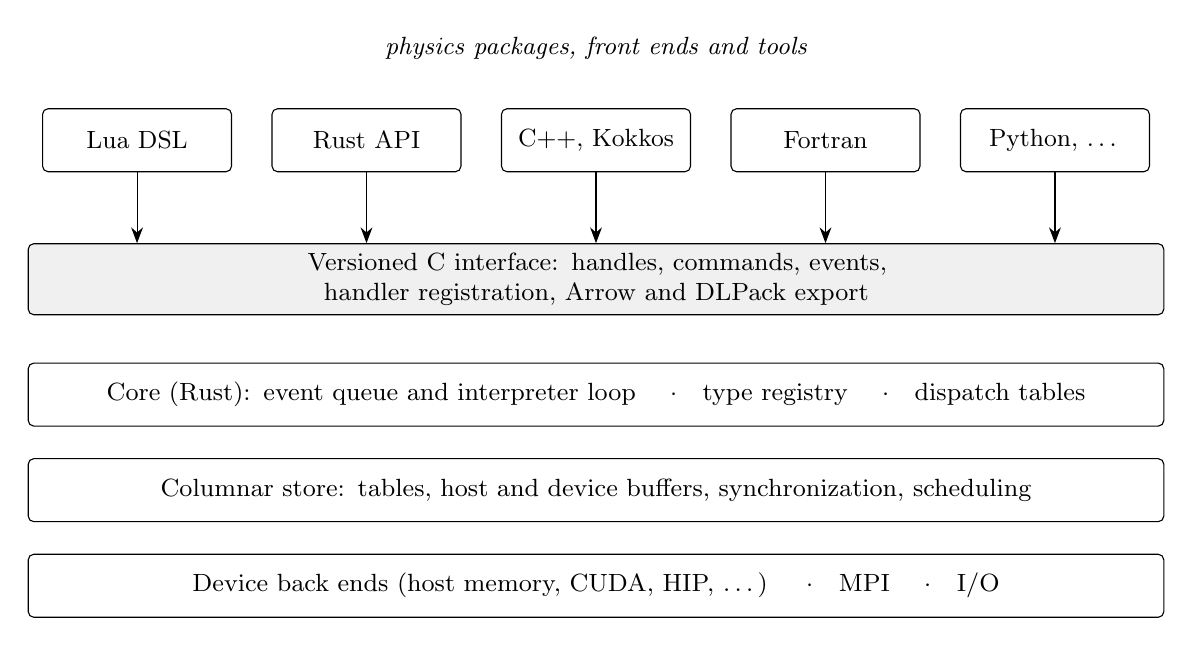
\begin{tikzpicture}[
  box/.style={draw, rounded corners=2pt, minimum height=8mm, align=center, font=\small, inner xsep=6pt},
  wide/.style={box, text width=140mm},
  >={Stealth[length=2mm]},
  node distance=6mm
]
  \node[wide] (core) {Core (Rust): event queue and interpreter loop \quad$\cdot$\quad type registry \quad$\cdot$\quad dispatch tables};
  \node[wide, below=4mm of core] (store) {Columnar store: tables, host and device buffers, synchronization, scheduling};
  \node[wide, below=4mm of store] (dev) {Device back ends (host memory, CUDA, HIP, \ldots) \quad$\cdot$\quad MPI \quad$\cdot$\quad I/O};
  \node[wide, above=6mm of core, fill=black!6] (cabi) {Versioned C interface: handles, commands, events, handler registration, Arrow and DLPack export};

  \node[box, above=9mm of cabi, minimum width=24mm] (fort) {C++, Kokkos};
  \node[box, left=5mm of fort, minimum width=24mm] (rust) {Rust API};
  \node[box, left=5mm of rust, minimum width=24mm] (lua) {Lua DSL};
  \node[box, right=5mm of fort, minimum width=24mm] (py) {Fortran};
  \node[box, right=5mm of py, minimum width=24mm] (jl) {Python, \ldots};

  \foreach \n in {lua,rust,fort,py,jl} \draw[->] (\n.south) -- (\n.south |- cabi.north);

  \node[above=5mm of fort, font=\small\itshape] {physics packages, front ends and tools};
\end{tikzpicture}
\caption{Proposed layering.  Everything above the shaded bar is a client of
the C interface; a Rust package may alternatively link the core statically.}
\label{fig:arch}
\end{figure}

\subsection{Alternatives considered}

\paragraph{Rust-specific stable ABIs.}  The \code{abi\_stable}~\cite{abistable}
and \code{stabby}~\cite{stabby} crates let Rust libraries exchange richer
types than C allows, with layout checks when a library is loaded.  They solve
Rust-to-Rust plugin loading only, which is not the problem \ref{req:lang}
poses.  They could later be used to make the Rust binding more comfortable.
The language-level proposal, \code{crabi}, remains experimental~\cite{crabi}.

\paragraph{WebAssembly components.}  The WebAssembly component model offers
exactly the language-neutral, versioned, typed interfaces this project wants,
and it is maturing: WASI~0.3, with native asynchronous calls, was released in
June 2026 and is enabled by default in Wasmtime~46~\cite{wasi03}.  It is
nevertheless the wrong tool for the data plane.  A component has its own
linear memory, so passing a column to it means copying; components cannot
reach GPU runtimes or MPI directly; and Fortran toolchain support is thin.  It
is worth revisiting for sandboxed control-plane extensions, where none of
those objections applies.

\paragraph{Remote procedure calls and serialization.}  Passing messages
between processes would give language neutrality at the price of copying all
data, which \ref{req:perf} rules out for anything but steering and
monitoring.

\subsection{Plugins}

A package should be loadable in two ways: linked into the executable when it
is built, or loaded from a shared library at run time by a DSL command.  In
both cases the package exposes one registration function that receives a
handle to the registry and uses it to define types, messages, handlers and new
DSL commands.  For a package whose definitions are written as a definition
script (Section~\ref{sec:scripts}), the registration function supplies that
script, embedded in the library, and registers the handlers it names; the
core then checks each handler's declared columns against the schema.  A package may also register initialization and finalization
hooks, which the core calls in a defined order relative to MPI and to other
packages; Section~\ref{sec:kokkos-needs} explains why these are needed.
Supporting static linking matters on machines where dynamic loading is
restricted or slow, which includes some of the largest ones.
Section~\ref{sec:build} describes how each configuration is linked and how
the process is started.

\subsection{Type checking across languages}
\label{sec:type-checking}

A C interface erases types.  To the linker a handler is an address and a
column is a buffer, and no compiler sees both sides of the boundary.  Types
cannot cross it, but descriptions of types can, as plain data, and the
schema is such a description.  Checking is therefore done in stages
(Table~\ref{tab:type-checking}): each language's compiler checks its own
side against a description generated from the schema, and the core checks,
when a package is loaded, that the description is still true.

\begin{table}[ht]
\centering
\small
\begin{tabularx}{\textwidth}{@{}>{\raggedright\arraybackslash}p{34mm} L >{\raggedright\arraybackslash}p{36mm}@{}}
\toprule
When & What is checked & By whom \\
\midrule
Compiling a package & The handler's code, against a typed header generated from the package's definition script & The package's own compiler \\
Loading a package & That the header was generated from the definitions now loaded; the handler's declaration against the schema; the interface version & The core \\
Each call & Nothing & \\
\bottomrule
\end{tabularx}
\caption{Stages of type checking across the language boundary.}
\label{tab:type-checking}
\end{table}

\paragraph{When a package is compiled.}  A definition script can be
evaluated offline, so a tool can turn it into a typed header for C++ and a
module for Fortran (Section~\ref{sec:scripts}).  A handler then obtains a
field through a generated accessor and not through a string.

\begin{itemize}
  \item \emph{C++.}  The accessor returns a Kokkos view of exactly the
        element type and shape of the field.  A misspelled field, or a
        wrong type, does not compile.
  \item \emph{Fortran.}  The generated module returns pointers of the right
        type, kind and rank, which the Fortran compiler checks.
  \item \emph{Rust.}  The generic interface is checked by the Rust compiler
        directly (Section~\ref{sec:mechanism}).
  \item \emph{Access.}  A column that the handler declared it only reads
        arrives as a view of constant elements, so that writing to it does
        not compile.
\end{itemize}

\paragraph{When a package is loaded.}  Checking at compile time proves only
that the code agrees with the header.  Two checks at load complete the
argument.

\begin{enumerate}
  \item \textbf{The hash.}  A plugin records a hash of the definition script
        it was built from.  The core compares it with the definitions that
        are loaded and refuses a plugin whose hash differs, so that a header
        which has gone out of date cannot pass.
  \item \textbf{The declaration.}  Each handler is registered with a
        declaration, as plain data: every column it reads and writes, with
        its element type, shape, unit and device
        (Section~\ref{sec:handlers}).  The core compares the declaration
        with the schema and resolves the names to column handles, once.  A
        mismatch is an error that names the package, the type and the
        field.
\end{enumerate}

The interface version is checked at the same moment, and structures passed
across the boundary carry their own size as their first field, so that a
newer core can serve an older plugin.  The header is a snapshot of the
schema and the hash is the proof that the snapshot is current.  Together
they give the effect of checking the whole program without a compiler that
sees the whole program, and because the checks are made at load, a call
costs nothing: by the time a handler runs, every name is a resolved
handle.

\paragraph{Without a generated header.}  A handler may instead look fields
up by name, as the sketch of Section~\ref{sec:kokkos} does.  The adapter
then checks the type the handler asked for against the type of the column,
once in each call.  That is a check for each table and not for each row,
and it finds at the first call what the generated header would have found
at compile time.  Plain C has no templates, and uses either generated
inline accessors or accessor functions for each element type, which fail
on a mismatch.

\paragraph{What this cannot catch.}

\begin{itemize}
  \item \emph{A handler that does not keep to its declaration.}  In C
        nothing prevents a handler from declaring a column of 64-bit
        floating-point numbers and then treating the buffer as something
        else.  The defenses are the unit test of each handler and the
        variant of the test scripts that runs under the address sanitizer
        (Section~\ref{sec:harness}).
  \item \emph{Dynamic languages.}  Python and Julia have no stage of
        compilation.  They receive columns through the Arrow and DLPack
        interfaces (Section~\ref{sec:schema}), which carry the element
        type, and are checked when the array is used.
\end{itemize}

%------------------------------------------------------------------------------
\section{C++ and Kokkos physics packages}
\label{sec:kokkos}

The working assumption is that most physics packages built on \camshaft{} will be
written in C++ and will use Kokkos for their kernels.  This section examines
how well the design serves them and what it must provide.  Nothing here has
been tested; milestones M4 and M5 (Section~\ref{sec:roadmap}) exist to test
it.

\subsection{Why the fit is good}

A Kokkos package is a plugin like any other.  It includes the generated C
header, registers handlers with C linkage, and runs Kokkos kernels inside
them.  Three properties of Kokkos make this natural.

\begin{itemize}
  \item \textbf{Kokkos can adopt memory it did not allocate.}  A
        \code{Kokkos::View} constructed from a raw pointer and extents is
        \emph{unmanaged}: it neither copies nor frees the
        memory~\cite{kokkosdocs}.  A handler
        can therefore wrap \camshaft{} columns as views at no cost, on the host or
        on a device.
  \item \textbf{The two data models agree.}  A \camshaft{} column is a contiguous,
        aligned, fixed-width buffer with an optional device copy, which is
        what a view is.  The host and device buffers of
        Section~\ref{sec:schema} were modeled on Kokkos's dual view in the
        first place.
  \item \textbf{The granularity matches.}  Kokkos parallelizes a loop over a
        range; \camshaft{} dispatches once per table and passes the handler a
        range of rows.  The handler body is one or a few
        \code{parallel\_for} calls.
\end{itemize}

Kokkos also supplies what Section~\ref{sec:gpu} found missing in Rust: one
double-precision kernel source for CUDA, HIP, SYCL and OpenMP.  For packages
that use it, risk~\ref{risk:gpu} in Section~\ref{sec:risks} largely disappears.
The package keeps access to the libraries built on Kokkos, and it gives up
little: templates cannot cross the C boundary, so nothing from \camshaft{} is
inlined into a kernel, which per-table dispatch never required.

The sketch below shows the shape of a handler.  All \camshaft{} names in it
are invented for illustration, and are explained after it.

\begin{lstlisting}[language=C++]
#include <Kokkos_Core.hpp>
#include <camshaft.h>            // generated C header
#include <camshaft_kokkos.hpp>   // header-only adapter (see below)

extern "C" cam_status advance(cam_batch* batch, void* /*ctx*/) try {
  // Unmanaged views over camshaft columns: no allocation, no copy.
  auto x = cam::view<double*[3]>(batch, "position");
  auto v = cam::view<const double*[3]>(batch, "velocity");
  const double dt = cam_batch_dt(batch);

  Kokkos::parallel_for("advance", x.extent(0), KOKKOS_LAMBDA(const int i) {
    for (int d = 0; d < 3; ++d) x(i, d) += dt * v(i, d);
  });
  return CAM_OK;
} catch (...) {
  return CAM_ERROR_PACKAGE;   // exceptions must not cross the C boundary
}
\end{lstlisting}

\code{advance} is the handler a package would register for a message such as
\code{pusher.advance} in the example of Section~\ref{sec:sketch}.  To keep
the sketch short, its body moves each particle by its velocity and applies
no force; it is not the Boris algorithm.  \code{cam\_batch} stands for what
a handler is given: a range of rows of one table, together with the columns
the handler declared.  \code{cam::view} is the adapter function that wraps
a column as an unmanaged view, and \code{cam\_batch\_dt} reads the time step
that the core chose for the current cycle (Section~\ref{sec:cycles}).  \code{cam\_status}, \code{CAM\_OK} and
\code{CAM\_ERROR\_PACKAGE} are the return codes of Section~\ref{sec:api}.
\code{camshaft.h} is the generated C header and \code{camshaft\_kokkos.hpp}
is the adapter's header.

\subsection{What the infrastructure must provide}
\label{sec:kokkos-needs}

Each item below is an obligation on \camshaft{} that the earlier sections did not
state, or stated only in general terms.

\paragraph{Runtime life cycle.}  Kokkos can be initialized at most once per
process, and should be initialized after MPI and finalized before MPI is
finalized~\cite{kokkosdocs}.  The
plugin interface therefore needs initialization and finalization hooks with a
defined order relative to MPI and to other plugins, in addition to the
registration function of Section~\ref{sec:api}.  \camshaft{} must also tell the
package which device it selected, so that Kokkos is initialized on the same
one.

\paragraph{One Kokkos per process.}  Kokkos keeps global state.  Two plugins
that each link their own copy, or that were built against different versions,
cannot safely share a process.  All Kokkos packages loaded together must use
one shared Kokkos library, and exactly one party must initialize it.  The
simplest rule is that \camshaft{} offers an optional Kokkos adapter which owns
initialization, and packages depend on that adapter.

\paragraph{Layout.}  A fixed-size-vector column stored in the Arrow manner is
interleaved ($x_0 y_0 z_0\, x_1 y_1 z_1 \ldots$), which Kokkos calls
\code{LayoutRight}.  On GPUs, Kokkos defaults to
\code{LayoutLeft}~\cite{kokkosdocs}.  The
adapter must construct views with the layout stated explicitly.  Whether
interleaved storage is the right default for vector fields, or whether each
component should be its own column, is a performance question for M1 and M5;
the schema should be able to express both.

\paragraph{One source of truth for synchronization.}  \camshaft{} tracks which of
a column's host and device buffers is current.  Kokkos's own
\code{DualView} does the same.  If a package used both, they would disagree.
Packages must take unmanaged views from \camshaft{} and declare their reads and
writes to it, and must not wrap \camshaft{} memory in a \code{DualView}.

\paragraph{Completion.}  A Kokkos kernel on a GPU may return before the work
is finished.  The scheduler needs to know when a handler's writes are
complete.  The simple contract is that a handler fences before it returns.
The better contract, which allows kernels on independent tables to overlap,
is for the handler to return a completion event; the Arrow device interface
already has a field for one.  The simple contract should come first.

\paragraph{Concurrency.}  Section~\ref{sec:schema} proposed running
independent kernels concurrently.  Kokkos has historically not supported
launching parallel regions from several host threads at once.  Its route to
doing so is separate execution-space instances, and the function that
creates them is still in Kokkos's experimental
namespace~\cite{kokkosdocs}.  Handlers must
therefore be able to declare that they are to be called from one thread at a
time, and that should be the default.  Concurrency between Kokkos kernels can
be revisited later through execution-space instances.

\paragraph{Host threads.}  A Kokkos OpenMP back end and a Rust thread pool
would each try to use every core.  When Kokkos packages are loaded, \camshaft{}
should not run its own data-parallel work at the same time as a handler, and
should let the adapter configure the thread count for both.

\paragraph{Errors.}  A C++ exception that propagates into Rust is undefined
behavior.  Handlers must catch everything and return an error code, as in
the sketch, and the adapter should provide a wrapper that does this so that
package authors cannot forget.  Section~\ref{sec:errors} adds checks that
can be made inside a kernel on a device.

\paragraph{Build.}  Kokkos packages are built with CMake.  \camshaft{} should
install its C header and library together with a CMake package configuration
file, so that a package finds it with \code{find\_package} and never needs to
invoke Cargo.

\subsection{Who allocates device memory}
\label{sec:kokkos-memory}

For a view to adopt a device buffer, the buffer must have been allocated in a
way the Kokkos back end accepts.  There are two ways to arrange that.

\begin{description}[style=nextline,leftmargin=2em]
  \item[The store allocates through the vendor runtime; Kokkos adopts.]
        This keeps C++ out of the allocation path.  It is straightforward for
        CUDA and HIP, where a pointer from the vendor allocator is valid
        throughout the process.  It is harder for SYCL, where memory belongs
        to a context and Kokkos must be using the same one; that requires
        passing a queue between the two, which has to be verified in M5.
  \item[Kokkos allocates; the store records.]
        The Kokkos adapter implements the device abstraction of
        Section~\ref{sec:gpu} using Kokkos's own allocation and copy
        functions (\code{kokkos\_malloc} and \code{deep\_copy}).  Every back end Kokkos supports then works
        without \camshaft{} knowing anything about it, including ones \camshaft{} has
        no vendor back end for.
\end{description}

Because the device abstraction is a table of C function pointers, both can be
supported, and the recommendation is to do so: vendor back ends for runs
without Kokkos, and the Kokkos-backed allocator as the default whenever the
adapter is loaded.  The second option is the lower-risk route to
\ref{req:port} given the working assumption of this section.

\subsection{The adapter, and the place of C++}

Package authors should not write the view-wrapping, exception-catching and
life-cycle code themselves.  \camshaft{} should ship a small Kokkos adapter: a
header that turns column handles into typed unmanaged views and wraps
handlers, and a small library that owns Kokkos initialization and implements
the Kokkos-backed allocator.  This is C++ code in the \camshaft{} repository, and
so it qualifies the brief's wish to avoid C++.  This has been accepted, on
the following terms: the adapter is a language binding, of the same standing
as the Fortran or Python bindings; it is optional; and the core neither
contains nor depends on any C++.  The alternative, leaving every package to write its
own adapter, would produce several incompatible ones and would break the
one-Kokkos-per-process rule.

\subsection{Kokkos from Rust}

If packages are in C++ and the core is in Rust, the remaining question is
what Rust packages should use.  Krokkos~\cite{krokkos}, the experimental Rust
interface to Kokkos, is directly relevant: if it matures, Rust and C++
packages could share one runtime, one allocator and one set of back ends
under \camshaft{}.  It should be evaluated alongside CubeCL and
\code{std::offload} in M5.

%------------------------------------------------------------------------------
\section{Packages and their dependencies}
\label{sec:packages}

Packages are not independent of one another.  The earlier sections already
let them depend on each other in three ways: a handler of one package reads
the columns of another (Section~\ref{sec:scripts}), one package answers a
message that another defines (Section~\ref{sec:dispatch}), and packages are
written against a protocol that another implements
(Section~\ref{sec:mesh-protocol}).  This section makes those dependencies
explicit.

\subsection{A directed graph without cycles}

A package declares what it requires, in its definition script: the other
packages it depends on and the external libraries it uses, each with the
versions it accepts.

\begin{lstlisting}[language={[5.3]Lua}]
-- In the definition script of package C.
cam.requires("A", ">= 2.0")
cam.requires("B", ">= 1.3")
\end{lstlisting}

The declarations form a directed graph.  It must have no cycles, and the
check invocation refuses a set of packages in which it has one.
Figure~\ref{fig:packages} shows an example.

\begin{figure}[ht]
\centering
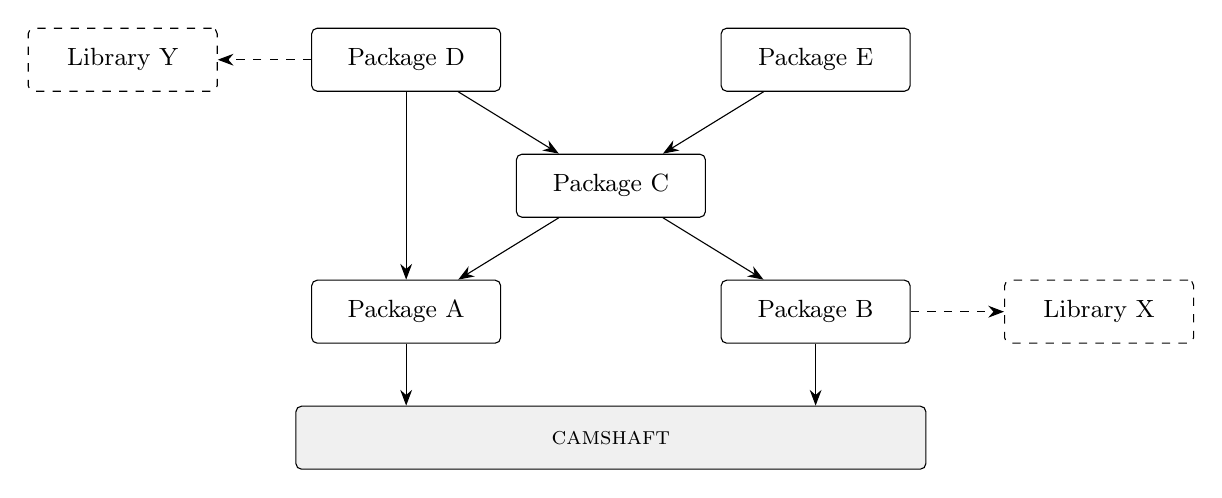
\begin{tikzpicture}[
  pkg/.style={draw, rounded corners=2pt, minimum height=8mm, minimum width=24mm, align=center, font=\small},
  ext/.style={pkg, dashed},
  >={Stealth[length=2mm]},
]
  \node[pkg, minimum width=80mm, fill=black!6] (core) at (0,0) {\camshaft{}};
  \node[pkg] (A) at (-2.6,1.6) {Package A};
  \node[pkg] (B) at (2.6,1.6) {Package B};
  \node[pkg] (C) at (0,3.2) {Package C};
  \node[pkg] (D) at (-2.6,4.8) {Package D};
  \node[pkg] (E) at (2.6,4.8) {Package E};
  \node[ext] (X) at (6.2,1.6) {Library X};
  \node[ext] (Y) at (-6.2,4.8) {Library Y};
  \draw[->] (A) -- (A |- core.north);
  \draw[->] (B) -- (B |- core.north);
  \draw[->] (C) -- (A);
  \draw[->] (C) -- (B);
  \draw[->] (D) -- (C);
  \draw[->] (D) -- (A);
  \draw[->] (E) -- (C);
  \draw[->, dashed] (B) -- (X);
  \draw[->, dashed] (D) -- (Y);
\end{tikzpicture}
\caption{An example of dependencies between packages.  An arrow points from
a package to what it depends on.  Dashed boxes are external libraries.  A
package may have several dependencies, as C and D do, so the structure is a
graph and not a tree; every package depends on \camshaft{}, directly or
through others.}
\label{fig:packages}
\end{figure}

\subsection{Tiers are left to protocols}

The core knows the graph and nothing else.  It has no notion of tiers and no
names for the kinds of package that occupy them, because different families
of packages need different arrangements, and Section~\ref{sec:mesh-protocol}
already keeps the meaning of data out of the core.

A family of packages agrees its own arrangement through \emph{protocols}.
Any package may publish one: a written statement of the tables, fields and
messages it provides, as the mesh protocol is.  A package then depends on a
protocol and not on a particular implementation of it, so that any package
which implements the protocol may be loaded in its place.

\subsection{What the graph determines}

\begin{itemize}
  \item \emph{Order.}  Packages are loaded, initialized and finalized in an
        order consistent with the graph (Section~\ref{sec:build}), and the
        default order of their handlers within a cycle follows it too
        (Section~\ref{sec:cycles}).
  \item \emph{Consistency before the run.}  The check invocation verifies
        that every requirement can be met by the set of packages a driver
        loads.  A plugin records the version of each dependency it was
        compiled against, and a mismatch is refused when the plugin is
        loaded (Section~\ref{sec:validation}).
  \item \emph{External libraries.}  Declaring them lets the core detect two
        packages that need incompatible versions of one library in one
        process, which the rule of one of each runtime forbids
        (Section~\ref{sec:build}), and lets output record what was used.  A
        library that keeps global state is initialized once, by the package
        or binding that owns it, as Kokkos is by its adapter
        (Section~\ref{sec:kokkos-needs}).
  \item \emph{Build and distribution.}  The same edges appear in each
        package's CMake configuration and in its Spack recipe
        (Section~\ref{sec:build}).
\end{itemize}

\paragraph{Mutual influence without a cycle.}  Two packages often need to
affect each other.  That does not require a cycle.  If A and C each act on
the other, A declares a message and C answers it.  C then depends on A, and
A depends on nothing above it: A sends its message without knowing who, if
anyone, will answer.

\subsection{Composition between packages}
\label{sec:composition}

Section~\ref{sec:dispatch-devices} established that a kernel cannot call a
handler.  A kernel of one package nevertheless often needs, for every
element, something that another package computes.  The graph gives the rule
for how it may get it.

\begin{table}[ht]
\centering
\small
\begin{tabularx}{\textwidth}{@{}>{\raggedright\arraybackslash}p{40mm} L L@{}}
\toprule
Direction & Means allowed & Why \\
\midrule
Downward, along a declared dependency & Composition at compile time: the dependent package includes inline functions that its dependency installs, and calls them inside its own kernels & The dependency is declared, its version is recorded and checked, and the call is static, so it works inside a kernel on a device \\
Upward or sideways, where no dependency is declared & Messages at the granularity of a table, or data: columns and look-up tables & The packages remain substitutable for one another and neutral as to language \\
\bottomrule
\end{tabularx}
\caption{How one package may use another.}
\label{tab:composition}
\end{table}

\paragraph{Downward.}  In Figure~\ref{fig:packages}, a kernel of C may call
an inline function of A for every element.  The call is resolved when C is
compiled and lies wholly outside dispatch.  Three conditions apply.  The
dependency must be declared.  The version that C was compiled against is
recorded in C's plugin and checked when it is loaded.  And the two are built
together, against the same Kokkos; the code that is inlined takes the
floating-point profile of the package that includes it
(Section~\ref{sec:floating-point}).  A package that offers itself for
composition installs its headers and a CMake package configuration, as
\camshaft{} itself does.

\paragraph{Upward or sideways.}  A package that needs something from a
package above it, or from a peer, has two means.  The first is a pair of
messages at the granularity of a table: its handler writes inputs to
columns, the other package's handler fills the outputs, and its next
handler continues.  The second is data: columns the other package
maintains, or a look-up table generated from records or imported from a
dataset (Sections~\ref{sec:records} and~\ref{sec:datasets}), read inside the
kernel.

\paragraph{The cost of the downward means.}  It is in practice confined to
C++, since inline functions and templates do not cross languages
(Section~\ref{sec:prior}); a package in another language uses messages or
data.  And a change low in the graph forces every package above it to be
rebuilt.  The rule accepts those costs only along edges that a package has
chosen to declare.

\subsection{Consequences for the design}

\begin{enumerate}
  \item Definition scripts declare requirements on packages and on external
        libraries, with versions.
  \item The core holds the graph, refuses a cycle, and orders loading,
        initialization and handlers by it.
  \item A plugin records the versions of its dependencies, and the core
        checks them at load.
  \item Any package may publish a protocol, and a package may depend on a
        protocol in place of an implementation.
  \item Composition at compile time is permitted along declared
        dependencies only; everything else passes through messages or
        data.
\end{enumerate}

%------------------------------------------------------------------------------
\section{Process and build model}
\label{sec:build}

The infrastructure drives the execution of the packages built on it, and
those packages are written in several languages.  That raises four practical
questions which the earlier sections left open: what the program's
\code{main} function is, who links the program, how a process containing
several language runtimes is started and stopped, and what build system the
project should use.

\subsection{The infrastructure is a library}

The answer to the first question is that \code{main} should contain almost
nothing.  Everything lives in a library, \code{libcamshaft}, behind the C
interface of Section~\ref{sec:api}.  The library offers one convenience entry
point that takes the command line and runs a script to completion, and
beneath it the individual steps (initialize, load a package, run a script or
a single command, finalize) so that a host can interleave its own work.
Three kinds of host then become possible.

\begin{table}[ht]
\centering
\small
\begin{tabularx}{\textwidth}{@{}l L L@{}}
\toprule
Host & What \code{main} is & When it is used \\
\midrule
Default executable & A Rust \code{main} of a few lines that calls the library & Normal use.  Packages are loaded from shared libraries at run time \\
Custom executable & A C, C++ or Fortran \code{main} that calls the library & Fully static builds; applications that embed \camshaft{} in a larger program \\
Foreign host & None of ours.  Python or Julia loads \code{libcamshaft} and drives it & Interactive work, notebooks, test harnesses, coupling to other tools \\
\bottomrule
\end{tabularx}
\caption{Hosts of the library.}
\label{tab:hosts}
\end{table}

This is the arrangement LAMMPS uses, a library with a trivial \code{main}
and a documented library interface~\cite{lammps}, and it is what makes
\ref{req:lang} hold for the host as well as for packages.  The question
\enquote{Rust's \code{main} or C's?} therefore has no single answer and does
not need one.  A Rust \code{main} is the right default: it is the simplest
thing to build, and a Rust library needs no runtime initialization when it is
called from a \code{main} written in another language, so nothing is lost in
the other two cases.

\subsection{Starting and stopping the process}

What matters is not who owns \code{main} but the order in which the library
brings the process up and takes it down, since the runtimes in the process
depend on one another.  The library should enforce this sequence:

\begin{enumerate}
  \item initialize MPI, with the thread-support level the loaded packages
        require, unless the host has already done so;
  \item select devices and run the initialization hooks of language bindings
        (the Kokkos adapter initializes Kokkos here, on the selected device);
  \item load packages and run their registration functions and
        initialization hooks, in the order of their dependencies
        (Section~\ref{sec:packages});
  \item run the interpreter loop;
  \item run finalization hooks in reverse order, then finalize the bindings,
        then MPI, unless the host owns it.
\end{enumerate}

Each language runtime has its own requirements, and the binding for that
language, not the package author, should meet them.

\begin{description}[style=nextline,leftmargin=2em]
  \item[Fortran.]
        Some compilers need their runtime library initialized explicitly when
        the main program is not Fortran.  Intel's documentation, for example,
        prescribes calls to \code{for\_rtl\_init\_} and
        \code{for\_rtl\_finish\_} and a link option to suppress the Fortran
        main~\cite{intelmixed}.  The Fortran binding's hooks are the place for
        this.
  \item[C++ and Kokkos.]
        Section~\ref{sec:kokkos-needs} covered Kokkos.  Static constructors
        and destructors in C++ packages run when the shared library is loaded
        and unloaded; packages should not depend on their order.
  \item[Julia.]
        Either Julia is the host and calls the library, or a Julia binding
        starts the Julia runtime in its initialization hook and Julia
        functions are registered as handlers through C-callable function
        pointers.  Compiling Julia packages ahead of time into shared
        libraries is possible with JuliaC, on Julia~1.12 or later, but the
        trimming that keeps such libraries small is still an experimental
        compiler feature~\cite{juliac}.
  \item[Python.]
        The same two options: Python as host, or an embedded interpreter
        started by a binding.  The first is much the more common need.
\end{description}

Three process-wide rules follow from sharing a process.  No package may
terminate the process itself; a fatal error is returned to the library, which
aborts through MPI so that every rank stops (Section~\ref{sec:errors}).  Signal handlers are installed
only by the library, since several of the runtimes above would otherwise
compete for them.  And interactive input is read on one rank only and
broadcast, so that the deterministic event ordering of
Section~\ref{sec:dispatch} is preserved.

\subsection{Linking}

\paragraph{The default configuration needs no mixed-language link.}  When
packages are plugins, each is a shared library linked by the tool that suits
its language, and that tool adds the language's own runtime libraries
(Table~\ref{tab:link}).  The only things shared between them are the C header
and \code{libcamshaft} itself.  Because Rust's standard library is linked
\emph{inside} \code{libcamshaft}, the library presents itself to every other
language as an ordinary C library with no visible Rust dependency.

\begin{table}[ht]
\centering
\small
\begin{tabularx}{\textwidth}{@{}L L@{}}
\toprule
Artifact & Linked by \\
\midrule
\code{libcamshaft} (shared and static) and the default executable & The Rust compiler, which invokes the C compiler driver, which invokes the system linker \\
Kokkos adapter; C++ packages & CMake, through the C++ compiler or the MPI wrapper for it \\
Fortran packages & The Fortran compiler driver or its MPI wrapper \\
Julia and Python packages & Nothing.  They load \code{libcamshaft} and register function pointers at run time \\
\bottomrule
\end{tabularx}
\caption{Who links what in the default, dynamic configuration.}
\label{tab:link}
\end{table}

The choice of linker proper is not a design decision.  The Rust compiler
delegates to the C compiler driver, and since version 1.90 uses LLD by
default on x86-64 Linux~\cite{rust190lld}; both can be overridden in Cargo's
configuration.  On systems where MPI and vendor libraries are supplied
through compiler wrappers, Cargo should be pointed at the wrapper as its
linker driver.

\paragraph{One copy of the core.}  A process must contain exactly one copy
of the core's state.  The executable and every plugin must therefore resolve
the C interface to the same \code{libcamshaft}, which is why it should normally
be a shared library that all of them link against, with a versioned name.

\paragraph{Rust packages.}  A Rust package has two routes, and they differ
in what is built.  As a plugin it is a shared library that talks to the core
through the C interface like any other; it carries its own copy of Rust's
standard library, which is harmless because only C types cross the boundary.
To use the generic Rust interface with full inlining
(Section~\ref{sec:dispatch}), it must instead be compiled by Cargo
\emph{together with} the core into one artifact, because Rust has no stable
ABI between separately compiled libraries.  In practice that means a small
\enquote{distribution} crate that depends on the core and on the chosen Rust
packages and produces the \code{libcamshaft} that everything else links against.

\paragraph{The static configuration.}  Some large machines discourage or
forbid dynamic loading.  There the whole program is one executable, and the
mixed-language link is unavoidable.  CMake should perform it, since it
computes the runtime libraries each language implicitly needs and links with
the appropriate driver.  Its inputs are the static \code{libcamshaft}, the
packages as static libraries, and a \code{main}.  Three points need care.

\begin{itemize}
  \item \emph{Only one Rust static library per link.}  A Rust static library
        contains the standard library and does not hide its internal symbols,
        so two of them in one link can conflict or silently override each
        other; the compiler options that would hide those symbols are still
        unstable~\cite{ruststaticlib}.  All Rust code in a
        static build must go through the single distribution crate described
        above.
  \item \emph{Registration must be explicit.}  Without dynamic loading there
        is nothing to find a package's registration function.  Relying on
        static constructors fails, because a linker omits archive members
        that nothing refers to.  The build should generate a table of
        registration functions from the list of configured packages and pass
        it to the library, as Cactus generates its thorn
        list~\cite{cactus}.
  \item \emph{The Rust static library has system dependencies} that the
        final link must name.  The Rust compiler can print them, and the
        installed CMake configuration file should record them.
\end{itemize}

\paragraph{One of each runtime.}  In either configuration a process should
contain one MPI library, one Kokkos, one OpenMP runtime and one C++ standard
library.  Two OpenMP runtimes in one process, typically one from a Fortran
compiler and one from a C++ compiler, is a well-known source of crashes and
oversubscription.  The build cannot fully prevent this, but the library can
detect the common cases when a package is loaded and refuse it with a clear
message.

\paragraph{Optimization across languages.}  Link-time optimization across
the Rust and C++ boundary is possible when both compilers share an LLVM
version, but the design does not need it: the boundary is crossed once per
table, not once per element.

\subsection{Build system}

\begin{table}[ht]
\centering
\small
\begin{tabularx}{\textwidth}{@{}l L L@{}}
\toprule
Option & For & Against \\
\midrule
Cargo only & Native to Rust; dependency management; testing & No install step for libraries and headers; no Fortran; knows nothing of Kokkos, MPI wrappers or GPU toolchains; build scripts can call other tools but that makes Cargo the outer build for C++ developers \\
CMake only & Native to Kokkos and to most scientific C++ and Fortran; computes mixed-language links & Rust development through CMake loses much of what Cargo provides \\
Meson & First-class support for Rust alongside C, C++ and Fortran & Kokkos and its ecosystem publish CMake packages; less familiar in this field \\
Bazel or Buck & Hermetic multi-language builds & Heavy; alien to supercomputer environments \\
Cargo and CMake, split by ownership & Each community keeps its own tool; neither build invokes the other in normal use & Two systems to maintain; the installed interface between them must be kept exact \\
\bottomrule
\end{tabularx}
\caption{Build-system options.}
\label{tab:buildsys}
\end{table}

Cargo is sufficient for the core and insufficient for the project.  The
recommendation is the last row of Table~\ref{tab:buildsys}.

\begin{description}[style=nextline,leftmargin=2em]
  \item[The core is a pure Cargo workspace.]
        It contains the core, the C interface, the Lua front end (Lua itself
        is compiled from vendored source by \code{mlua}, needing only a C
        compiler), the Rust interface and the default executable.
        \code{cargo build} and \code{cargo test} work with no other tool.
  \item[Installation is an explicit, separate step.]
        Cargo does not install libraries.  \code{cargo-c} builds the shared
        and static libraries, generates the header and a pkg-config file, and
        installs them with correct library versioning~\cite{cargoc}.  The
        installation must also include a CMake package configuration file and
        the \emph{source} of the Fortran interface module, since compiled
        Fortran module files are specific to one compiler.
  \item[Bindings and packages in C++ and Fortran use CMake.]
        They find an installed \camshaft{} with \code{find\_package} and link to
        it as an imported target.  They never invoke Cargo and need no Rust
        toolchain.
  \item[Inside the repository, CMake can build the core too.]
        The adapter's CMake project can use Corrosion, which imports a Cargo
        crate as a CMake target~\cite{corrosion}, so that a C++ developer
        working on the adapter builds everything with one command.  This is
        a convenience; the installed interface remains the contract.
  \item[Julia and Python need no build integration.]
        They load the installed library.  Each binding is an ordinary package
        in its own ecosystem.
  \item[Distribution is through Spack.]
        Spack is how supercomputing sites install software and already
        understands both Cargo and CMake packages~\cite{spack}.
        Section~\ref{sec:containers} says how containers relate to it.
\end{description}

One number must be shared by all of this: the interface version.  It should
be defined once, in the Cargo manifest, and propagated from there to the
header, the library's versioned name, the pkg-config and CMake files, and the
check that the core performs when a plugin registers.

The repository layout that follows from these choices is sketched below.

\begin{lstlisting}
camshaft/
  Cargo.toml            workspace
  crates/
    camshaft-core/      registry, store, events, dispatch
    camshaft-capi/      the C interface; header generated from here
    camshaft-lua/       Lua front end
    camshaft/           Rust interface and default executable
    camshaft-dist/      distribution crate: core + compiled-in Rust packages
  bindings/
    kokkos/             CMake; header-only adapter and small library
    fortran/            CMake; interface module source
    python/  julia/     packages in their own ecosystems
  examples/             one small package per language
  tests/                test scripts and baseline summaries
  xtask/                the test orchestrator, a Rust program
  docs/                 portal and narrative documentation (mdBook)
  design/               this report
\end{lstlisting}

\subsection{Consequences for the design}

\begin{enumerate}
  \item The C interface gains host entry points: a run-to-completion call
        and the individual initialize, load, run and finalize steps, each
        usable when the host already owns MPI.
  \item Every binding has initialization and finalization hooks of its own,
        distinct from those of packages, and the library fixes their order.
  \item The library accepts a table of statically linked registration
        functions as an alternative to loading shared libraries.
  \item The interface version is checked at registration, and the library
        checks for duplicated runtimes when loading a package.
  \item Installation produces the shared and static libraries, the header,
        pkg-config and CMake files, and the Fortran module source.
\end{enumerate}

%------------------------------------------------------------------------------
\section{Containers}
\label{sec:containers}

A container image fixes a software stack so that it can be reproduced and
moved.  This section records a strategy.  Only one image is made now, the
one in which the project is built and tested; images for running are
deferred.

\subsection{Where containers help, and where they are hard}

They help in three places: a reproducible environment for building, images
for continuous integration (Section~\ref{sec:ci}), and easy use on
workstations and in clouds.  On large machines four things are hard.

\begin{itemize}
  \item \emph{MPI.}  For performance a container must use the MPI of its
        host.  Apptainer documents two ways of doing so: a compatible MPI
        inside the image that cooperates with the host's launcher, or no
        MPI in the image and the host's library bound into
        it~\cite{apptainermpi}.  Both depend on the binary compatibility of
        the two libraries.  MPICH is the open reference implementation,
        and the vendor libraries derived from it (Cray MPICH, Intel MPI,
        MVAPICH) share its binary interface~\cite{mpichabi}; Open MPI does
        not, so an image built for one family does not run with the other.
  \item \emph{GPUs.}  Apptainer binds the host's driver libraries into the
        container, with one option for NVIDIA and another for AMD.  The
        application must have been built for a version of CUDA or ROCm that
        the host's driver supports~\cite{apptainergpu}.  Each back end
        therefore needs an image of its own.
  \item \emph{The C library.}  Libraries bound in from the host were built
        against the host's C library, and Apptainer warns that the versions
        in the container and on the host \enquote{must not be too far
        apart}~\cite{apptainergpu}.  A container whose C library is older
        than the host's is the usual failure.
  \item \emph{Tuning and licenses.}  An image built for a generic processor
        gives up optimization for a particular one, and some vendor
        compilers and libraries may not be redistributed in an image.
\end{itemize}

\subsection{What the design already provides}

\begin{itemize}
  \item \emph{The MPI~5.0 ABI.}  Section~\ref{sec:mpi} plans a direct
        binding to the standard ABI.  An image built against it runs with
        any host MPI that implements it, which removes the division into
        families.
  \item \emph{A C interface between the core and plugins}
        (Section~\ref{sec:api}).  An image of the core is neutral, and the
        Kokkos adapter and the packages are layers for each back end.
  \item \emph{The search path for datasets} (Section~\ref{sec:datasets}).
        Data is mounted when a container runs and is never part of an
        image, which is the only possibility for data that is licensed or
        very large.
  \item \emph{Spack as the route for distribution}
        (Section~\ref{sec:build}).  Spack generates a recipe for an image
        from the description of an environment~\cite{spackcontainers}, so
        images and native installations come from one description.
\end{itemize}

\subsection{Strategy}

\begin{enumerate}
  \item \textbf{An image for building and testing, now.}  It holds the
        compilers, an installed \camshaft{} with its CMake configuration,
        and the Kokkos adapter, and it is the image that continuous
        integration uses from M0.  Packages are built inside it and not on
        the host, which keeps to one Kokkos, one OpenMP runtime and one C++
        standard library, as Section~\ref{sec:build} requires.
  \item \textbf{Images for running, later.}  One for each back end,
        generated from the Spack environment.  These are deferred until a
        milestone that has a GPU.
  \item \textbf{Provenance.}  The digest of the image, with the hashes of
        the datasets in use, is recorded in every output file.
  \item \textbf{No promise of one image for every machine.}  The kernel, the
        drivers and the interconnect of the host still decide what works.
        Spack remains the primary route on the largest machines.
\end{enumerate}

%------------------------------------------------------------------------------
\section{Distributed memory}
\label{sec:mpi}

MPI remains the only distributed-memory layer available on every
high-performance machine, and \camshaft{} must use it.  The state of the Rust
bindings (Section~\ref{sec:language}) matters less than it seems, for two
reasons.

First, MPI~5.0, approved in June 2025, standardizes the ABI: one header and
one set of type and constant definitions, valid for every conforming
implementation~\cite{mpi50,mpiabi}.  MPICH has implemented it since version
5.0.0, released in February 2026~\cite{mpich5}.  Open MPI has added it for
its 6.0 series, which had not been released when this was written, and so
far for C only: its change log notes that the Fortran bindings are not yet
covered~\cite{ompi6}.  That gap does not affect a binding from Rust, which
uses the C interface.  Against a standard
ABI, a Rust binding no longer needs to discover each implementation's
definitions when it is built; the interface can be declared once.  The part of
MPI that an infrastructure layer needs (communicators, non-blocking
point-to-point, collectives, and parallel I/O via a library) is small enough
to bind directly.

Second, the design already hides MPI.  Packages do not call MPI; they declare
which columns are exchanged, and the store performs the exchange.  MPI
therefore sits behind one internal interface and could be supplemented later
by another transport without affecting packages.

The recommendation is to begin with \code{rsmpi}~\cite{rsmpi} for speed of
prototyping, behind an internal trait, and to plan a thin direct binding to
the MPI~5.0 ABI once implementations of it are widespread.

%------------------------------------------------------------------------------
\section{Meshes}
\label{sec:mesh}

Meshes are the most demanding data the infrastructure will hold, and a
package devoted to mesh generation is expected to be built on it.  This
section examines whether the table model of Section~\ref{sec:schema} is
adequate for structured, adaptive and unstructured meshes, and what has to be
added.  The conclusion is that the model is adequate with three additions:
\emph{relations} between tables as a declared kind of column, \emph{index
spaces} that span several tables, and a protocol for \emph{change}, since
adaptive meshes alter the number and identity of rows during a run.

\subsection{Prior art}

\begin{table}[ht]
\centering
\small
\begin{tabularx}{\textwidth}{@{}l L L@{}}
\toprule
System & Mesh kind & Representation \\
\midrule
AMReX~\cite{amrex} & Patch-based structured AMR~\cite{bergercolella} & Levels of rectangular boxes of varying size; connectivity implicit within a box \\
Parthenon~\cite{parthenon} & Block-based structured AMR & Tree of blocks of identical size, packed into one array for bulk kernels \\
p4est~\cite{p4est} & Forest of octrees & Leaves stored as a sorted array along a space-filling curve; no pointers \\
PETSc DMPlex~\cite{dmplex} & Unstructured, any dimension and cell type & All entities numbered in one index space; adjacency stored as offset and index arrays \\
MOAB~\cite{moab} & Unstructured & Entities grouped by type in contiguous ranges; data as \enquote{tags}; arbitrary entity sets \\
PUMI~\cite{pumi} & Unstructured, adaptive & Full adjacencies; every entity classified on a geometric model entity \\
Omega\_h~\cite{omegah} & Simplex, adaptive, on GPUs & Arrays only, on Kokkos; adaptation as bulk array operations \\
Conduit Blueprint~\cite{blueprint} & All of the above & A naming convention for describing mesh arrays in memory, not a data structure \\
\bottomrule
\end{tabularx}
\caption{Mesh systems examined.}
\label{tab:mesh}
\end{table}

Three lessons follow from Table~\ref{tab:mesh}.

\begin{enumerate}
  \item \emph{Array-based representations are the ones that reach GPUs.}
        p4est, DMPlex, MOAB and Omega\_h all store connectivity as flat arrays
        of integers.  Omega\_h shows that even conforming adaptation of an
        unstructured mesh can be expressed as bulk operations that build new
        arrays from old ones.  Pointer-based mesh structures have no path to
        a device.
  \item \emph{Grouping entities by type is universal.}  MOAB's ranges, DMPlex's
        strata and the \enquote{element blocks} of the common file formats
        are all the same idea, and it is the table of
        Section~\ref{sec:schema}.
  \item \emph{A shared convention is worth more than a shared library.}
        Blueprint lets independent codes exchange meshes because they agree
        on what the arrays are called and what they mean.  \camshaft{} needs the
        equivalent (Section~\ref{sec:mesh-protocol}).
\end{enumerate}

\subsection{Relations}
\label{sec:relations}

Connectivity is a relation between the rows of two tables: a cell and its
nodes, a face and its two cells, a node and the cells around it.
Section~\ref{sec:schema} allowed an object to \enquote{refer to rows in
another table}; meshes require that to be a first-class, declared part of the
schema.  Three forms are needed.

\begin{description}[style=nextline,leftmargin=2em]
  \item[Fixed arity.]
        Every row refers to the same number of targets: a tetrahedron has four
        nodes.  This is a column whose element is a fixed-size array of row
        indices, which the schema already supports.
  \item[Variable arity.]
        Rows refer to differing numbers of targets: the cells around a node,
        the faces of a polyhedron.  The representation is the one every
        array-based mesh library and every sparse-matrix library uses: an
        array of offsets, one per row plus one, and an array of target
        indices.  It is also exactly the layout of Arrow's variable-size list
        type~\cite{arrowcolumnar}, so it remains exportable without copying,
        and both arrays are plain fixed-width buffers that work on a device.
  \item[Implicit.]
        In a structured block, the neighbor of cell $(i,j,k)$ is found by
        arithmetic.  Nothing is stored.  The schema records only the block's
        shape, and kernels compute neighbors themselves.
\end{description}

The restriction in Section~\ref{sec:schema} therefore stands in spirit:
columns hold fixed-width data, there are no pointers, and variable-length
data is admitted only in offsets-and-values form.

\paragraph{What declaring a relation buys.}  A relation column is declared
with its target, as a foreign key is in a database.  That declaration is what
allows the infrastructure, and not each package, to do the following.

\begin{itemize}
  \item \emph{Renumber and compact.}  When the rows of a table are reordered
        (for cache locality, along a space-filling curve) or deleted, every
        relation that targets it is rewritten automatically.
  \item \emph{Migrate.}  When rows move to another MPI rank, the rows they
        depend on can be found and sent with them, and indices translated
        between local and global numbering.
  \item \emph{Build ghost layers.}  The rows needed from neighboring ranks
        are those reachable through declared relations from locally owned
        rows.
  \item \emph{Validate and persist.}  Indices can be range-checked in debug
        builds, and files can be written and read with relations intact.
\end{itemize}

\paragraph{Operations on relations.}  A relation is a sparse boolean matrix,
and the operations a mesh package needs most are matrix operations.
Transposition turns cell-to-node into node-to-cell.  Composition turns
cell-to-face and face-to-cell into cell-to-cell.  Which adjacencies to store
and which to derive is the mesh package's decision.  DMPlex stores only the
relations between entities of adjacent dimension, in both directions, and
obtains the rest by traversal~\cite{dmplex}; MOAB stores each element's
vertices and derives most other adjacencies on demand~\cite{moab}.  The
infrastructure should provide transpose,
compose and sort as bulk operations on the host.  Device versions raise the
kernel-technology question of Section~\ref{sec:gpu} for the core itself and
should be decided in M5; until then a mesh package can supply its own through
the Kokkos adapter.

\paragraph{Index width.}  Local row indices should default to 32 bits, which
halves the memory traffic of every gather and is what GPU codes use; global
identifiers must be 64 bits.  The schema should let a relation declare its
width.

\subsection{Index spaces and mixed element types}

A mesh of tetrahedra and hexahedra is naturally two tables, since the two
have different node counts and need different kernels.  Per-table dispatch
(Section~\ref{sec:dispatch}) then does the right thing without further
design: the message \enquote{assemble} resolves to one handler for the
tetrahedron table and another for the hexahedron table.

The difficulty is on the other side of the relation.  A face must be able to
refer to \enquote{a cell} without knowing which table it is in.  The
recommendation is an \emph{index space}: a contiguous numbering that spans
several tables, each occupying a sub-range.  A relation targets an index
space; the table and local row follow from the sub-range.  This is how
DMPlex's point numbering and MOAB's entity handles work.

Mixed meshes also bear on risk~\ref{risk:dispatch} in Section~\ref{sec:risks}.  A mesh
with a handful of element types is a handful of large tables, which is the
favorable case.  A mesh partitioned into thousands of small material
regions, each a table, is not, and the model should prefer a material column
within one table to a table per material.

\paragraph{Subsets.}  Boundary conditions and material regions apply a
handler to part of a table.  Two mechanisms are needed: a tag column with
rows kept sorted by it, so that each subset is a contiguous range and kernels
remain simple loops; and explicit index lists for subsets that overlap or
cannot be sorted.  The event model already allows a target to be a set of
rows.

\subsection{Structured and block-structured adaptive meshes}

There are three families, and they fit the table model to different degrees.

\paragraph{Block-based.}  The mesh is a tree of blocks, all with the same
number of cells.  This fits best.  One table holds the blocks, one row each,
with columns for level, logical position and neighbors.  A field is a column
whose element is a fixed-size array of the block's cells, so the field data
for all blocks is one contiguous buffer indexed by block and by cell.  That
is precisely the packed layout Parthenon builds so that one kernel launch
covers every block~\cite{parthenon}, and it is a four-dimensional unmanaged
Kokkos view.  Refinement replaces one row by $2^d$ rows.

\paragraph{Tree-based, cell by cell.}  The mesh is the set of leaves of an
octree or a forest of them.  One row per leaf, sorted along a space-filling
curve, with level and position as columns, is the p4est
representation~\cite{p4est} and is a table as it stands.  Neighbor relations
are either searched for by key or stored as a relation that is rebuilt after
each adaptation.

\paragraph{Patch-based.}  The mesh at each level is a union of rectangular
boxes of differing sizes~\cite{bergercolella,amrex}.  A field is then a
variable-length array per row with a per-row shape.  The offsets-and-values
form of Section~\ref{sec:relations} can hold it, but kernels must loop over
boxes individually, as AMReX does.  The model supports this family less
gracefully than the other two, and that should be accepted, not designed
around.

In all three, ghost cells belong inside the per-block array, filling them is a
message that the mesh package answers, and coarse--fine operations
(prolongation, restriction, flux correction) are messages dispatched on the
field's type.

\subsection{Unstructured adaptation}

Refining or coarsening an unstructured mesh changes topology: entities are
created and destroyed, and relations change.  There are two ways to do it,
and the store must support both.

\emph{Bulk rebuild.}  Mark entities; compute the new tables and relations
from the old in parallel; swap them in.  This is Omega\_h's
method~\cite{omegah}; it is the one that runs on GPUs and it suits a columnar
store exactly, since nothing is modified in place.

\emph{Incremental edit.}  Insert and delete individual rows, as a Delaunay
or advancing-front generator does.  This needs deletion without immediate
compaction (a tombstone and a free list), spare capacity in each column, and
a later compaction step that renumbers through the declared relations.  It is
inherently a host-side, mostly serial activity.

\subsection{Change over time}
\label{sec:mesh-change}

Adaptive meshes are where the event-driven design earns its place, because
adaptation is a sequence of steps contributed by different packages.  It
should be a standard sequence of messages:

\begin{enumerate}
  \item \emph{flag}: physics packages mark rows for refinement or coarsening;
  \item \emph{adapt}: the mesh package builds the new tables and, for each, a
        \emph{transfer map} relating new rows to old ones;
  \item \emph{transfer}: each field is carried across the transfer map by a
        handler chosen by the field's declared transfer rule (inject,
        interpolate, conserve, one that a package supplies, or, for an
        analytic field, evaluation afresh as in
        Section~\ref{sec:expressions});
  \item \emph{rebalance}: rows are repartitioned and migrated;
  \item \emph{changed}: everything that depends on the mesh is told.
\end{enumerate}

The transfer map is itself a relation, so nothing new is needed to store it.
Two things are new.  Every table needs a version counter that is incremented
when its rows change, and everything derived from a table (cached dispatch
lists, exchange plans, derived relations, device buffers, a package's own
workspace) must record the version it was built from, so that stale data is
detected and not silently used.  And each field's schema entry needs a
transfer rule alongside the placement and life-cycle metadata listed in
Section~\ref{sec:schema}.

Row counts that change at run time also affect device memory.  Reallocating
device buffers at every adaptation is expensive, so columns need a capacity
larger than their length and a growth policy, and the Kokkos adapter must hand
out views of the current length over buffers of larger capacity.

\subsection{Distributed meshes}

Section~\ref{sec:mpi} said that packages declare which columns are exchanged
and the store performs the exchange.  For meshes this needs to be made
concrete.

\begin{itemize}
  \item Every row of a distributed table has a 64-bit global identifier and
        an owner.  Rows present on a rank that it does not own are ghosts.
  \item The pattern of an exchange is itself a relation, from each ghost row
        to its owner on another rank.  PETSc's star forest~\cite{petscsf}
        shows that this one abstraction covers ghost updates, assembly of
        contributions back to owners, and migration.  \camshaft{} should adopt
        it as the single communication primitive for tables.
  \item Partitioning is a decision, not a mechanism.  The mesh package
        chooses the partitioner (a space-filling curve for trees and blocks, a
        graph partitioner for unstructured meshes) and gives the store a
        destination rank for each row.  Migration, with dependent rows found
        through declared relations, is then generic.
\end{itemize}

\subsection{A mesh-generation package}

A generator places demands that a solver does not.

\paragraph{It should not be forced to live in tables.}  Generation
algorithms such as Delaunay insertion and advancing front are irregular and
pointer-heavy, and mature generators exist with their own internal
structures (Gmsh~\cite{gmsh}, for example, offers a C interface).  The
package must be free to compute however it likes and \emph{publish} the
result.  What the infrastructure owes it is a fast way in: bulk creation of
tables from arrays, and adoption of buffers the package already holds,
without copying.  The Arrow C data interface provides the latter, since it
works in both directions and carries a release callback so that ownership
passes cleanly.

\paragraph{It needs the incremental-edit path} of the previous subsection for
algorithms that do operate on tables, such as local refinement, smoothing
and quality improvement, and those are also the algorithms worth running in
parallel and on devices.

\paragraph{It needs geometry.}  A generated mesh is usable for adaptation
and boundary conditions only if each boundary entity records the geometric
entity (the CAD face, edge or vertex) it lies on, as PUMI
requires~\cite{pumi}.  That classification is a pair of ordinary columns.
The geometric model itself is opaque to the infrastructure and belongs to
the mesh package, which answers messages such as \enquote{project this point
to its surface} during adaptation.

\paragraph{It needs to read and write the standard formats.}  The file
formats group elements into blocks by type and name boundary subsets, which
maps directly onto tables and subsets.  Section~\ref{sec:interchange}
describes how a mesh produced by another program is brought in.

\subsection{The mesh protocol}
\label{sec:mesh-protocol}

If the mesh package defines the mesh tables, every physics package depends on
that one package, and a second mesh package (a structured one beside an
unstructured one, say) cannot be substituted.  The remedy is the Blueprint
lesson: a \emph{mesh protocol}, which is a written convention and not code.
It states what tables, columns, relations and index spaces a mesh of each
kind exposes, by what names, with what meaning, and which messages a mesh
package must answer (the sequence of Section~\ref{sec:mesh-change}, ghost
filling, geometric queries, the projection of expressions onto its tables as
in Section~\ref{sec:expressions}).  Physics packages are written against the
protocol; mesh packages implement it.  Section~\ref{sec:packages} makes
protocols available to any package.

The protocol should be specified alongside the infrastructure but stay out of
the core, which should know about relations, index spaces and versions and
nothing about cells or faces.  That keeps the core equally useful for
particles, for networks, and for whatever comes later.

\subsection{Consequences for the design}

\begin{enumerate}
  \item The schema gains relation columns (fixed-arity, variable-arity) with
        declared targets, index spaces spanning tables, per-relation index
        width, and a transfer rule per field.
  \item The store gains renumbering and compaction through relations,
        tombstoned deletion, column capacity distinct from length, table
        version counters, and import of external buffers.
  \item The core gains bulk relation operations and a single
        ghost-to-owner communication primitive.
  \item The standard event vocabulary gains the adaptation sequence.
  \item A mesh protocol is written as a separate specification.
\end{enumerate}

None of these contradicts an earlier recommendation.  The division of labor
is that the infrastructure understands \emph{structure} (tables, relations,
ownership, versions) and the mesh package understands \emph{meaning}
(topology, geometry, quality, refinement criteria).

%------------------------------------------------------------------------------
\section{Expressions and analytic fields}
\label{sec:expressions}

Users will want to give a field by a formula: an initial density, a
time-dependent drive, an exact solution to compare against.  An
\emph{analytic field} is a field whose values are given by a formula in
space, time and other data, and not by stored state.
Section~\ref{sec:dsl} ruled out calling Lua for each element.  This section
says what is done instead.

\subsection{Expressions, not callbacks}

The driver does not hand the core a function to call.  It builds an
\emph{expression}: a tree whose leaves are coordinates, time and constants,
and whose nodes are operations.  Coordinates and time are symbolic values,
and arithmetic on them builds the tree.  Lua runs once, to build it, and
plays no part in evaluating it.  This is the staging pattern of Regent and
Terra (Section~\ref{sec:prior}).  The tree is data in the registry, as a
record is, and that is the source of every advantage below: it can be
checked before the run, evaluated on a device, recorded in the output and
evaluated again whenever it is needed.

\begin{lstlisting}[language={[5.3]Lua}]
-- Symbolic coordinates and time.  With units = true they are quantities.
local x, y, z, t = cam.coordinates{ units = true }
local w   = cam.quantity(2.0, "mm")
local rho = cam.quantity(1.2, "kg/m^3") * cam.exp(-(x^2 + y^2) / w^2)

-- An initial condition: evaluated once, before the first cycle.
mesh.cells:set("density", rho)

-- A field the driver adds, kept current in every cycle.
local E0    = cam.quantity(1.0e5, "V/m")
local omega = cam.quantity(2.0e9, "rad/s")
mesh.cells:define("drive", E0 * cam.sin(omega * t), { refresh = "cycle" })
\end{lstlisting}

In the sketch \code{mesh.cells} stands for a table of cells that a mesh
package exposes, and the names of the functions are placeholders, as in
Section~\ref{sec:sketch}.

\paragraph{Tracing.}  A user may also write an ordinary Lua function.  The
core calls it once, with symbolic arguments, and records the tree that
results.  In the driver's environment the mathematical library accepts
symbolic values, so a function written for numbers usually traces as it
stands.  What cannot be traced is a decision that depends on a value.  Lua
converts the result of every comparison to a boolean~\cite{lua55}, so a
comparison cannot be made to build a tree, and an \code{if} on a symbolic
value has nothing to test.  Comparisons are therefore functions, and a
piecewise field is written with \code{cam.where}, which takes a condition
and two expressions.  An attempt to branch on a symbolic value is an error
when the driver is checked, with a message that says so.

\paragraph{Leaves.}  The leaves of an expression may be more than
coordinates and time.

\begin{itemize}
  \item \emph{Parameters and the fields of records}, which become constants
        of the tree.
  \item \emph{Other columns.}  An expression over existing columns is a
        derived field, such as a kinetic energy formed from a density and a
        velocity.
  \item \emph{Tabulated data}, through a node that interpolates.
  \item \emph{A random source} keyed by the global identifier of the row,
        of the counter-based kind~\cite{random123}, so that the values do
        not depend on how the mesh is partitioned.
\end{itemize}

\subsection{Operators and functions}
\label{sec:expr-functions}

An expression may use the arithmetic of Lua and the numerical functions of
its mathematical library~\cite{lua55}.

\begin{itemize}
  \item \emph{Operators}: \code{+}, \code{-}, \code{*}, \code{/},
        \code{\textasciicircum}, unary minus, the modulo operator \code{\%}
        and floor division \code{//}.  Lua allows each of these to be
        redefined for a new kind of value, which is how they come to build
        a tree.
  \item \emph{Functions of Lua's library}: \code{abs}, \code{floor},
        \code{ceil}, \code{sqrt}, \code{exp}, \code{log}, \code{sin},
        \code{cos}, \code{tan}, \code{asin}, \code{acos}, \code{atan},
        \code{min}, \code{max}, \code{fmod}, \code{modf}, \code{frexp},
        \code{ldexp}, \code{deg} and \code{rad}, and the constants
        \code{pi} and \code{huge}.
  \item \emph{Functions Lua lacks}: the hyperbolic functions, the error
        function, \code{hypot}, a sign function and others of the kind are
        supplied by \code{cam}.
\end{itemize}

The rule for admitting a function is that every evaluator, on the host and
on a device, implements it, and implements the same definition.  The two
forms of modulo show why the definition matters.  The operator \code{\%}
is the remainder of a division that rounds toward minus infinity, so its
result has the sign of the divisor; \code{fmod} is the remainder of a
division that rounds toward zero, so its result has the sign of the
dividend, as in C.  An expression keeps whichever the user wrote.

Three things are excluded.

\begin{enumerate}
  \item \textbf{Comparisons and logic.}  The comparison operators, and
        \code{and}, \code{or} and \code{not}, cannot build a tree, for the
        reason given above.  They are available as functions, with
        \code{cam.where} to choose between two expressions.
  \item \textbf{\code{math.random}.}  It is replaced by the random source
        keyed by global identifier.
  \item \textbf{Functions that inspect a number}: \code{math.type},
        \code{math.tointeger} and \code{math.ult} have no meaning for a
        symbolic value, and using one is an error.
\end{enumerate}

Transcendental functions may differ in their last bits between the
mathematical libraries of a host and of a device.  An expression evaluated
on a GPU is therefore not guaranteed to match its evaluation on the host
bit for bit, and tests that compare the two must allow for it.

\subsection{To a kernel, a column}

A kernel is compiled code that reads columns and nothing else
(Section~\ref{sec:handlers}), so an analytic field reaches it as a column.  The
expression is evaluated into the column under a \emph{refresh policy}:
once, for an initial condition; in every cycle, for a field that depends on
time; or whenever the table changes.  The version counters of
Section~\ref{sec:mesh-change} tell the core when a column is stale.  After
the mesh is adapted, the transfer rule of an analytic field is to evaluate
it afresh on the new rows, not to interpolate from the old ones.

\paragraph{Time.}  By default a field refreshed in every cycle is evaluated
at the time at which the cycle starts.  An integrator with several stages
needs it at intermediate times, so a package may ask for an analytic field
to be evaluated at a stated time.

\subsection{The function and its sampling}

A formula is defined over space and time.  A mesh supplies only the points
at which it is sampled, and there is more than one reasonable choice: the
centers of cells, the nodes, quadrature points, the positions of particles.
What is wanted may not be a sample at all.  A finite-volume method wants
the average of the function over each cell, and a finite-element method
wants a projection onto its basis.

The division of labor is the one Section~\ref{sec:mesh} draws between
structure and meaning.  The core evaluates an expression at any column of
points it is given.  The mesh or physics package decides which points, and
how the samples become the values of the field, by answering a projection
message that the mesh protocol defines (Section~\ref{sec:mesh-protocol}).

\subsection{Units}

Units in expressions are opt-in, and the rules extend those for driver
scripts in Section~\ref{sec:validation}.

\begin{enumerate}
  \item \textbf{Without units, everything is a bare number.}  Coordinates
        are numbers in the unit of the mesh's coordinates, time is a number
        in the unit of the clock, and the result is taken in the unit of
        the field it fills.  Nothing is checked.
  \item \textbf{With units, the whole expression is checked.}  When the
        driver asks for dimensioned coordinates, every value in the tree
        has a dimension (Section~\ref{sec:units}).  The exponential of a
        length is an error, adding a bare number to a length is an error,
        and the dimension of the result must be that of the field.
        Trigonometric functions accept an angle or a dimensionless number,
        which is taken to be in radians.
  \item \textbf{Conversion costs nothing at run time.}  Conversion factors
        are folded into the constants of the tree when it is built.
\end{enumerate}

With units, each operator and function has a rule for dimensions.
Table~\ref{tab:expr-units} gives those that are not obvious.

\begin{table}[ht]
\centering
\small
\begin{tabularx}{\textwidth}{@{}>{\raggedright\arraybackslash}p{44mm} L@{}}
\toprule
Operation & Rule when units are in use \\
\midrule
\code{\%}, \code{//}, \code{fmod} & Both arguments must have the same dimension.  \code{\%} and \code{fmod} return that dimension, which is what a periodic profile such as \code{x \% wavelength} needs; \code{//} returns a dimensionless number \\
\code{floor}, \code{ceil}, \code{modf} & The argument must be dimensionless, since the floor of a length would depend on the unit it was expressed in \\
\code{sqrt}, and \code{\textasciicircum} with a constant exponent & The dimension is raised to the power, so dimensions carry rational exponents \\
\code{\textasciicircum} with any other exponent, \code{exp}, \code{log} & The arguments must be dimensionless \\
\code{min}, \code{max}, \code{abs} & The arguments must share a dimension, which the result keeps \\
\code{atan} with two arguments & The arguments must share a dimension, and the result is an angle \\
\bottomrule
\end{tabularx}
\caption{Dimension rules for operators and functions in expressions.}
\label{tab:expr-units}
\end{table}

The check is made on the tree, when the driver is checked, and does not
require the expression to be evaluated anywhere.  This is the principal
gain over a callback, whose units could be examined only at the points at
which it happened to be called.

\subsection{Evaluation}

There are three ways to evaluate a tree, and they should be built in this
order.

\begin{enumerate}
  \item \textbf{A host evaluator in the core}, which works through the tree
        a column at a time, so that each operation is one loop over a
        buffer.
  \item \textbf{A device evaluator in the Kokkos adapter}, a small
        interpreter that runs for each element inside a single kernel.
        This needs no compilation at run time and works on every back end
        Kokkos supports.  AMReX's parser, which WarpX uses for analytic
        density and field profiles, evaluates expressions supplied at run
        time on GPUs from several vendors~\cite{amrexparser,warpxparams}.
  \item \textbf{Generated kernels.}  The check invocation, or a preparation
        step like it, can write a handler and its kernel for each expression in a driver
        and compile it into a small plugin before the run is submitted.
        This is the fastest route and can wait until measurement shows that
        the second is too slow.
\end{enumerate}

\subsection{Checking}

\begin{itemize}
  \item \emph{When the driver is checked}: that the names in an expression
        exist, that its dimensions are consistent, that its result suits
        the field, and that no branch was attempted on a symbolic value.
  \item \emph{In the pre-flight}: failures that depend on the data, such as
        the square root of a negative number, appear only on evaluation.
        Columns filled before the first cycle are checked then for values
        that are not finite and for the ranges their fields declare, so
        that a bad initial condition stops the run at cycle~0.
\end{itemize}

\subsection{The fill on the host}

Some functions cannot be traced and have no form as an expression: a loop
that runs until an iteration converges, a call into other Lua code, a read
from a file.  For these one exception to the rule of Section~\ref{sec:dsl}
is allowed.  The driver may give an ordinary Lua function, which is called
with numbers, once for each row, on the host, to fill a column.

\begin{lstlisting}[language={[5.3]Lua}]
mesh.cells:fill_on_host("density", function(x, y, z)
  local rho = 1.0
  repeat                              -- runs until converged: untraceable
    local step = f(rho, x, y) / df(rho, x, y)
    rho = rho - step
  until math.abs(step) < 1e-12
  return rho
end)
\end{lstlisting}

The exception is bounded in four ways.

\begin{itemize}
  \item \emph{It has an explicit name.}  A function given where an
        expression is expected is traced, and if it cannot be traced that
        is an error.  The fill on the host happens only when it is asked
        for by name.
  \item \emph{It is for fills made once.}  It cannot have a refresh policy,
        and it cannot be evaluated afresh after the mesh is adapted.
  \item \emph{It runs on the host.}  A column that lives on a device is
        filled on the host and copied.
  \item \emph{It carries no units.}  The function receives bare numbers and
        returns one, which is taken in the unit of the field.
\end{itemize}

It costs one call into Lua for every row, which is tolerable once and would
be ruinous in every cycle.  It is also checked less well than an
expression: a mistake that shows only at certain positions is found during
the real fill, which is before the first cycle but after the wait in the
queue.  Three measures reduce that.  The check invocation calls the
function at several points across the extent of the domain, not at one.  It
times those calls and reports an estimate of the time the fill will take on
each rank.  And the pre-flight checks the filled column as it does any
other.  The output records where in the script the function was given,
since there is no formula to record.

A user for whom neither an expression nor this fill will do can compute the
values elsewhere and import them, from a database file
(Section~\ref{sec:interchange}) or with Python as the host
(Section~\ref{sec:build}), or can supply a compiled handler in a package.

\subsection{Consequences for the design}

\begin{enumerate}
  \item The registry holds expressions, and the C interface can create and
        evaluate them.
  \item The driver's environment supplies symbolic coordinates and time, a
        mathematical library that accepts symbolic values, comparison
        functions and \code{cam.where}, and traces a function given where
        an expression is expected.  The operators and functions of
        Section~\ref{sec:expr-functions} are implemented, to one
        definition, by every evaluator.
  \item A field may be bound to an expression with a refresh policy, and
        \enquote{evaluate afresh} joins the transfer rules.
  \item The core has a host evaluator; the Kokkos adapter has a device
        evaluator.
  \item The mesh protocol gains a projection message.
  \item The pre-flight checks columns filled before the first cycle.
  \item A fill on the host by an untraced function exists under an explicit
        name, for fills made once.
\end{enumerate}

%------------------------------------------------------------------------------
\section{Checkpoints, restart and database files}
\label{sec:checkpoint}

Three needs are met by one mechanism: saving a run so that it can continue
later, changing a run at the point where it continues, and starting a run
from data that another program prepared.  In each case the object is a
\emph{database file}: the store, written out with enough beside it to be
understood without the program that wrote it.

\subsection{What a checkpoint holds}
\label{sec:checkpoint-holds}

A checkpoint is more than the tables.

\begin{itemize}
  \item The \emph{effective schema}: the definitions of every package
        together with whatever the driver added, in the machine-readable
        form of Section~\ref{sec:docs}.
  \item The records, the cycle counter and the clock
        (Sections~\ref{sec:records} and~\ref{sec:cycles}).
  \item The expressions behind analytic fields, with their refresh policies
        (Section~\ref{sec:expressions}).
  \item The text of the driver script and of every modification script, and
        the journal of commands executed (Section~\ref{sec:replay}).
  \item The system of units of each package and the version of the
        physical constants (Section~\ref{sec:units}).
  \item The name, version and hash of every external dataset in use, but
        not its contents (Section~\ref{sec:datasets}).
\end{itemize}

It is also less than the tables.  What can be rebuilt is not written: ghost
rows, derived relations, generated look-up tables, exchange plans and the
copies of columns on a device.  Nor is every field written.  Each field has
a \emph{persistence class}, which its owner declares.

\begin{description}[style=nextline,leftmargin=2em]
  \item[State.]
        The default.  The field is written to every checkpoint.
  \item[Derived.]
        The field is not written.  It declares how it is rebuilt: by an
        expression, or by a handler that a package supplies.
  \item[Scratch.]
        The field is not written and has no meaning from one cycle to the
        next.  At a restart it is filled with values that are not numbers,
        so that a kernel which reads it before writing it is found at once.
\end{description}

A flag that merely excluded a field would be dangerous, because excluding a
field that is in fact state breaks restarts without any sign.  The classes
make the developer say why a field is left out, and the restart test of
Section~\ref{sec:replay} finds a field that was classed wrongly.  A driver
may ask for more fields to be written, for debugging, and declares the
class of the fields it adds itself.  It may not exclude a package's state.

Anything a package holds outside the store is lost at a restart.  A package
with such state must move it into fields or records when it receives the
message that announces a checkpoint.

\subsection{Writing a checkpoint}

Checkpoints are written only between cycles (Section~\ref{sec:cycles}),
when every package is in a consistent state.  A driver asks for one by
command, as the sketch of Section~\ref{sec:sketch} does after a stop on the
wall clock, or at intervals through the triggers of
Section~\ref{sec:cycles}.  Writing is a standard sequence.

\begin{enumerate}
  \item Packages are told that a checkpoint is about to be written, and
        move any state of their own into the store.
  \item Columns whose current copy is on a device are brought to the host,
        one column at a time, so that the host never holds a second copy of
        everything.
  \item The schema, the records, the journal and the state fields are
        written.
  \item A checksum and a mark of completion are written last.  The file is
        written under a temporary name and renamed, and the last few
        checkpoints are kept, so that a failure during writing never
        destroys the only good one.
\end{enumerate}

\paragraph{Format.}  HDF5 is the first format~\cite{hdf5}: one dataset for
each column, one group for each table, the schema and the journal beside
them.  It is read and written from every language, which matters for
Section~\ref{sec:interchange}.  The writer sits behind an internal
interface, as MPI does (Section~\ref{sec:mpi}).  Whether one shared HDF5
file performs adequately on the largest machines is not assumed, and the
interface leaves room for ADIOS2~\cite{adios2} as a second format.

\paragraph{Checkpoints are not output.}  A checkpoint holds all state at
full precision, exists so that a run can continue, and is kept in small
numbers.  An output file holds the fields a user selected, exists to be
analyzed, and is kept in large numbers.  The same writer serves both; they
differ in what is selected.

\subsection{Restart by replay}
\label{sec:replay}

Restoring the data is the easy half of a restart.  The hard half is the
driver, which is a program: it may run, create objects and run again, and a
checkpoint may fall anywhere in that.  Standard Lua has no means of saving
a program in the middle of its execution; even its function for saving a
single function does not save the variables the function
captured~\cite{lua55}.

The decision is to restart by \emph{replay}.  The same driver script is
executed again from its first line, against a journal that the checkpoint
carries.  There is no separate restart script.  LAMMPS takes the other
course, a second input script that reads the restart file, and its
documentation lists what the user must then specify again by hand: fixes,
computes, variables, regions and the settings for
output~\cite{lammpsrestart}.

\paragraph{The journal.}  The checkpoint records, in order, each command
the driver completed and the result it returned.  On replay there are two
kinds of command.

\begin{itemize}
  \item \emph{Commands that change the database}: creating a table or rows,
        setting a field, deleting, writing a checkpoint.  Their effects are
        already in the checkpoint.  On replay they are not executed.  Each
        returns its recorded result, and a handle it returned is bound to
        the restored object.
  \item \emph{Commands that change only the process}: loading a package,
        registering a handler written in Lua.  Their effects are not in any
        file.  They are executed again in every session.
\end{itemize}

The \code{run} that was interrupted resumes with what remains of it.  The
journal records the cycle at which it began, so relative limits
(Section~\ref{sec:cycles}) are honored as well as absolute ones.

\paragraph{A driver that was edited.}  Replay compares each command with
the journal.  A change to a command that was completed is an error, which
names the first command that differs, because the past cannot be changed.
The stop conditions of the interrupted \code{run} may be changed, and that
is how a run is extended.  Everything after it is free.

\paragraph{One rule for users.}  The state of Lua variables does not
survive a restart.  Whatever must survive belongs in a record.

\paragraph{A different layout.}  The store owns partitioning and placement,
so a checkpoint can be read on a different number of ranks or on a
different device.  The results are then no longer identical bit for bit,
since the order of floating-point operations changes; LAMMPS documents the
same of its own restarts~\cite{lammpsrestart}.

\paragraph{The restart test.}  Run twenty cycles.  Separately run ten,
restart, and run ten more.  Compare the two bit for bit, on the same layout.
A difference means that state is missing from the store or that a field has
the wrong persistence class.  The test is cheap, and every package should
run it in continuous integration (Section~\ref{sec:ci}).

\subsection{Modification scripts}
\label{sec:modification}

A user may want to change a run where it restarts: alter existing objects,
create new ones, delete some.  This needs no new kind of script.  A
\emph{modification script} is a batch of commands in the driver role
(Section~\ref{sec:scripts}) that is injected at a boundary between cycles.
A restart is simply the commonest moment to inject one.

The program of a run is then its driver followed by its modification
scripts, in order.  The checkpoint stores the text of each and the cycle at
which it was applied.

\begin{lstlisting}
job 1:  driver.lua runs to cycle 4000 and checkpoints (wall clock)
job 2:  restart with M1.lua  ->  M1 applied at cycle 4000, recorded; runs to 7000
job 3:  restart, no options  ->  driver replayed, M1 replayed, resumes at 7000
\end{lstlisting}

\begin{itemize}
  \item \emph{It is replayed like the driver.}  In the third job the
        commands of M1 that change the database are not executed, and any
        handlers it registered are registered again.
  \item \emph{It is applied once.}  A script is known by a hash of its
        text.  If a job script that is resubmitted in a chain names M1
        again, the core recognizes it and refuses, so a modification cannot
        be applied a second time by accident.
  \item \emph{It sees the database, not the driver's variables.}  It finds
        objects by name.
  \item \emph{It is checked before the job is submitted.}  The check
        invocation reads the schema, the records and the row counts of the
        checkpoint into its shadow state (Section~\ref{sec:validation}),
        replays the driver on it, applies the modification, continues
        through the rest of the driver and calls every handler.  A
        modification that deletes a table the driver uses later is found
        there.
  \item \emph{The run remains reproducible.}  Running the driver from the
        beginning with the recorded modifications applies each at its
        recorded cycle.
\end{itemize}

\paragraph{What may be modified.}  Deletion cannot be unrestricted.
Removing the cells of a mesh row by row would break a topology that only
the mesh package understands.  Two controls apply.

\begin{itemize}
  \item \emph{The owner of a type decides whether a driver may create and
        delete its rows directly.}  For a type such as a particle it
        usually may.  For the entities of a mesh the owner will usually
        require that changes go through the package's own commands.
  \item \emph{A field declares whether its value may change after a run has
        started.}  Parthenon makes the same distinction among its
        parameters~\cite{parthenondocs}.
\end{itemize}

After a modification the versions of the tables it touched are advanced,
packages are told that they changed (Section~\ref{sec:mesh-change}), and
the pre-flight checks of Section~\ref{sec:preflight} are made again before
the run continues.

\subsection{Matching a file to its schema}
\label{sec:file-schema}

A file carries its schema, not merely a version number.  For each package
it also records the package's version, the schema version and the hash of
the definition script.  When a file is read, each type in it is compared
with the definitions that are loaded, and there are four outcomes.

\begin{enumerate}
  \item The hashes are identical, and reading proceeds.
  \item The file has an older schema version and a migration exists.  The
        data are migrated in memory, and the file is not altered.
  \item The schema differs but the schema version is the same.  The file is
        refused: a definition was changed without a new version, which is
        what the compatibility check of Section~\ref{sec:validation} exists
        to prevent.
  \item The file is newer than the code.  It is refused.
\end{enumerate}

Fields are matched by their stable identifiers, not by position.  A field
added in a newer version is filled from its default, so that only renaming
a field or changing its meaning requires a migration to be written.  Units
are recorded with every field, so a change of unit is a conversion
(Section~\ref{sec:units}).  The fields and types a driver added are
recorded with their namespace and matched to the driver's commands on
replay.  The layout of the file has a version number of its own, distinct
from those of the packages.  A file without its mark of completion, or
whose checksum fails, is rejected.  The check invocation reports all of
this on a login node, before a job is submitted.

\subsection{Database files as the interchange format}
\label{sec:interchange}

The describe invocation already emits the schema of a package
(Section~\ref{sec:docs}).  It can also write a database file that contains
the schema and no rows.  That file is a \emph{template}, and it makes
starting from prepared data the same operation as restarting: a file filled
by another program is a checkpoint at cycle~0.  No separate path for
importing is needed.

\paragraph{Meshes from other programs.}  This is the main use, since a mesh
is often generated by a program outside \camshaft{}.

\begin{itemize}
  \item \emph{For a program the user writes, the template is the
        interface.}  A preprocessor in Python opens it, finds the tables
        and fields by name, and writes arrays into them.
  \item \emph{Existing generators write their own formats,} so a converter
        is still needed.  The mesh package offers an import command for the
        standard formats, and the template is what its converters produce.
  \item \emph{Only the state fields need be supplied.}  A program supplies
        nodes, the connectivity of cells and the tags of boundaries.  Faces,
        adjacencies, global identifiers and the partition are derived by
        the mesh package when the file is loaded.  The persistence classes
        of Section~\ref{sec:checkpoint-holds} are what tell an external
        program which fields it must write.
  \item \emph{A filled file is validated before a job is submitted.}  It is
        only data, so the check invocation can verify its structure (index
        ranges, units, constraints) and call the mesh package's own
        validation (orientation, positive volumes) on a login node.
\end{itemize}

The interchange format is HDF5 whatever format large checkpoints use,
because programs in every language can write it.

\subsection{Consequences for the design}

\begin{enumerate}
  \item Every field has a persistence class, and a derived field declares
        how it is rebuilt.
  \item Every file carries the effective schema, the versions and hashes of
        its packages, a checksum and a mark of completion.
  \item The core keeps a journal, and every command, including those that
        packages add, declares whether it changes the database or only the
        process.
  \item A restart executes the same driver against the journal.
  \item Modification scripts are injected at a boundary between cycles,
        applied once, recorded in the checkpoint, and checked against the
        checkpoint beforehand.
  \item A type declares whether drivers may create and delete its rows, and
        a field whether it may change after the start.
  \item The describe invocation writes a template file, and a run may start
        from any database file whose schema matches.
\end{enumerate}

%------------------------------------------------------------------------------
\section{External datasets}
\label{sec:datasets}

Many packages depend on data they do not own: tables for an equation of
state, opacities, cross sections, interatomic potentials.  Such data is
often large, has versions of its own, and is frequently licensed in a way
that forbids redistributing it.  It is read while the program runs.

\subsection{Declared, not opened}

A package should not open a file at a path of its own choosing.  That
hides the dependency from the check invocation, lets a thousand ranks parse
the same file, and ties the package to the layout of one site.  A package
instead declares each \emph{dataset} in its definition script
(Section~\ref{sec:scripts}): a name, a format, the versions it accepts,
whether it is required, and documentation that says where to obtain it and
under what license.

\begin{lstlisting}[language={[5.3]Lua}]
cam.dataset("pusher.cross-sections", {
  format   = "hdf5",
  versions = ">= 2.1",
  required = true,
  doc = "Collision cross sections.  Licensed; see the package's guide.",
})
\end{lstlisting}

Names are resolved to locations through a search path, which a site's
configuration, an environment variable or the driver sets.  LAMMPS finds
its potential files in this way, through a list of directories in an
environment variable~\cite{lammpspaircoeff}.  The generated documentation
of a package lists its datasets (Section~\ref{sec:docs}).

\subsection{Checked before the run}

The check invocation confirms that each dataset is found, can be read, and
passes a probe that the package supplies: that it has the right format and
version, and contains what the driver asks of it.  The pre-flight repeats
the test on the compute nodes, because the file systems mounted there are
not always those of the login nodes (Section~\ref{sec:validation}).

\subsection{Imported into the store}

\begin{itemize}
  \item \emph{Read once.}  The package's reader, which knows the format,
        runs on one rank, and the result is distributed.  A failure to read
        is then an orderly error by construction
        (Section~\ref{sec:errors}).
  \item \emph{Held as a replicated table.}  The data becomes a bulk table of
        which every rank holds the whole, as the generated look-up tables
        of Section~\ref{sec:records} are.  It thereby gains what any table
        has: declared units, converted on import
        (Section~\ref{sec:units}), and a copy on a device for kernels that
        run there.
  \item \emph{One copy for each node.}  The ranks of a node share one copy
        through the shared memory that MPI provides~\cite{mpi50}, so that a
        large table is not held once for every rank.
\end{itemize}

\subsection{Datasets and files}

An imported dataset is never written to a checkpoint.  Its persistence
class is derived (Section~\ref{sec:checkpoint-holds}), and its rule for
rebuilding is to import it again.  The checkpoint records the name, the
version and a hash of each dataset.  A restart verifies the hash, so a
table that was changed between two jobs is detected, and output files
record the same identities for provenance.  A dataset may also be declared
as not to be exported, in which case a driver cannot ask for its table to
be written to any file; licensed data then stays where its license allows.

\subsection{Errors and tests}

The kinds of error that a dataset can cause are declared like any others
(Section~\ref{sec:errors}): not found, wrong format, wrong version, a hash
that does not match, and a look-up outside the range of a table during a
run.  The last is found by a check inside the kernel, which names the row.

A public repository cannot hold licensed tables.  A package therefore
ships small substitutes that carry no license, for its tests, and a test
that needs the real data is reported as skipped when the data is absent
(Section~\ref{sec:harness}).

\subsection{Consequences for the design}

\begin{enumerate}
  \item Definition scripts declare datasets, and a search path resolves
        their names.
  \item A package supplies a probe and a reader for each dataset.
  \item The store has replicated tables, held once for each node.
  \item Checkpoints and output files record the identity of each dataset
        and not its contents, and a dataset can be barred from export.
  \item The check invocation and the pre-flight both verify datasets.
\end{enumerate}

%------------------------------------------------------------------------------
\section{Validation}
\label{sec:validation}

\ref{req:early} asks that errors be caught as early as possible.  The
reason is an asymmetry of cost.  A simulation that fails at its hundredth
cycle has already waited in a queue and spent part of an allocation, and
its author learns of one mistake at a time.  A check made on a login node
costs seconds and can report every mistake it finds.  The design should
therefore spend effort freely on checks made before a run, and should treat
any error first reported during a run as one that an earlier stage ought to
have caught, wherever that was possible.  The rule is this.

\begin{quote}
\emph{Every check is made at the earliest stage at which the information it
needs exists.  Nothing is left to the run that could have been caught
before it.}
\end{quote}

\subsection{Stages}

Table~\ref{tab:stages} lists the stages in order and what each can check.
Several of the checks were introduced in earlier sections for other
reasons: bindings checked when a package is loaded
(Section~\ref{sec:scripts}), the interface version
(Section~\ref{sec:api}), duplicated runtimes (Section~\ref{sec:build}),
ownership of types (Section~\ref{sec:scripts}), and the range-checking of
relations and the detection of stale versions (Section~\ref{sec:mesh}).
They are gathered here because they are one policy.

\begin{table}[ht]
\centering
\small
\begin{tabularx}{\textwidth}{@{}>{\raggedright\arraybackslash}p{30mm} L >{\raggedright\arraybackslash}p{30mm}@{}}
\toprule
Stage & What is checked & What it needs \\
\midrule
Compilation & In the core, memory errors and data races, by the Rust compiler.  In packages, the names and types of fields, through the header generated from the definitions (Section~\ref{sec:scripts}) & Compilers only \\
Definition check & Names; namespaces and ownership; that the dependencies between packages form no cycle and their version requirements can be met; the fixed-width rule for bulk types; the targets of relations; dimensions and units; defaults that break their own constraints; missing documentation & Nothing: no MPI and no device \\
Schema compatibility & A field removed or changed since the last release without a new schema version and a migration & The description of the previous release \\
Loading a package & Each handler's declared columns, with their types and units, against the schema; the versions of the packages it was compiled against; the hash of the definition script; the interface version; duplicated runtimes & The compiled plugin \\
Driver check & The arguments of every command; references to tables, records and names; that files exist; that every dataset is found and passes its package's probe; that a checkpoint's schema matches; a modification script, against the checkpoint it will be applied to; the dimensions of every expression; every Lua handler, by calling it once & A login node, for seconds \\
Pre-flight & That every record is complete; that every message which will be sent has a handler for the device each of its tables is on; that exchange plans can be built; that datasets can be read from the compute nodes; that columns filled before the first cycle are finite and within their declared ranges & The real run, before its first cycle \\
During the run & Index ranges, in debug builds; stale versions; that the ranks agree on the sequence of events; constraints on columns, on request & The real run \\
\bottomrule
\end{tabularx}
\caption{Stages of checking, earliest first.}
\label{tab:stages}
\end{table}

The schema compatibility check does for definitions what the comparison of
binary interfaces in Section~\ref{sec:ci} does for the C interface: it
compares the machine-readable description of a package
(Section~\ref{sec:docs}) with that of its last release.

\subsection{Constraints are data}

Constraints are treated as documentation is: as data in the registry, read
by one piece of code.

\begin{itemize}
  \item \emph{Constraints are metadata on fields.}  A field already has a
        type, a unit, a default and its documentation.  It may also be
        required, have a permitted range or a set of permitted values, and
        be marked as deprecated (Section~\ref{sec:schema-record}).
  \item \emph{The arguments of a command are a record.}  A command such as
        \code{run} declares a record type for its arguments
        (Section~\ref{sec:records}), so validating a command is validating
        a record against its type, and a package that adds a command gets
        the validation with it.
  \item \emph{There is one validator, and it is in the core.}  It stands
        behind the C interface, so a Python or Julia host and a C++ package
        are checked exactly as a Lua script is.
  \item \emph{Rules that span fields need a function.}  \enquote{Exactly
        one of these two must be given} cannot be stated field by field.  A
        type may register a validation function, in the definition script
        or compiled, which is called once for each record and never once
        for each row.
  \item \emph{References are checked through declared relations.}  A
        boundary condition that names a missing boundary, or a cell that
        refers to a missing material, is found by the same mechanism that
        range-checks any relation (Section~\ref{sec:relations}).
\end{itemize}

Because constraints are data, the generated documentation shows them, and
the description of a parameter that a user reads is the rule by which their
input is judged.

\begin{lstlisting}[language={[5.3]Lua}]
cam.param("pusher.cfl", cam.f64, {
  default = 0.5,
  min = 0.0, max = 1.0, exclusive_min = true,
  doc = "Time-step limit as a fraction of the stability bound.",
})
\end{lstlisting}

\subsection{Units in driver scripts}

Section~\ref{sec:units} sets out the model: a field states its kind of
quantity and takes its unit from the package's system of units, unless it
names a unit explicitly.  Three rules govern what a driver may write.

\begin{enumerate}
  \item \textbf{A bare number is in the field's unit.}  Driver scripts are
        not required to attach units to quantities.
  \item \textbf{An explicit quantity is converted.}  A value given with a
        unit of the right dimension is converted to the field's unit when
        it enters the record.
  \item \textbf{A dimension mismatch is rejected,} at the user's line.
\end{enumerate}

\begin{lstlisting}[language={[5.3]Lua}]
-- pusher.Species declares mass as a mass.  The package's system of units is
-- the SI, so the field's unit is the kilogram.
{ name = "electron", mass = 9.109e-31 }                     -- kilograms
{ name = "electron", mass = cam.quantity(9.109e-28, "g") }  -- converted
{ name = "electron", mass = cam.quantity(1.0, "m") }        -- rejected
\end{lstlisting}

Conversion happens in the control plane, where a value enters a record.
Columns are stored in their units and nothing is converted inside a kernel.
Between packages the same principle is applied one stage earlier: a handler
declares the unit it expects of a column, the binding check compares it
with the column's unit when the package is loaded, and a mismatch is an
error then.  A value given in a unit that belongs to another system of
quantities is rejected in the same way, since no factor converts it.

\subsection{Strict script environments}
\label{sec:strict}

Lua is permissive in ways that hide mistakes until late.  The environments
in which definition and driver scripts run (Section~\ref{sec:scripts}) must
close each of them.

\begin{itemize}
  \item \emph{Unknown arguments are rejected.}  Lua accepts any key in a
        table, so a misspelled argument would be ignored in silence and its
        default used.  Every command rejects a key it does not declare.
        This is the most valuable single check.
  \item \emph{Undefined names are errors.}  Reading a global variable that
        was never set, or a member that a package or a type does not have,
        yields \code{nil} in Lua and a confusing failure somewhere later.
        In these environments both are errors where they occur, and
        assigning to an undeclared global is an error too.
  \item \emph{Numbers are converted strictly.}  A value such as \code{1e6}
        is accepted where an integer is expected, because it is one.  A
        value with a fractional part is not, and neither is one that does
        not fit.
  \item \emph{Errors point at the user's line.}  A report names the file and
        line of the call in the user's script, the command and the argument,
        what was expected and what was given, the nearest valid name, and
        the argument's own documentation.  Every kind of error has a stable
        identifier, which tests that expect a rejection name
        (Section~\ref{sec:harness}).
\end{itemize}

\begin{lstlisting}
run.lua:14: cam.run: unknown argument 'untill_time'
  did you mean 'until_time'?  Absolute limit on simulation time.
\end{lstlisting}

The same environments protect the assumption of Section~\ref{sec:dispatch}
that every rank processes the same sequence of events.  A script is read on
one rank and sent to the others, so all of them run the same text.  Library
functions whose results could differ between ranks (the time of day,
unseeded random numbers, reading files) are removed or replaced by versions
that give every rank the same answer.  And during a run the ranks compare a
hash of the events they have processed at intervals, so that a divergence
is reported when it happens and not when its consequences appear.

\subsection{The driver check}

A driver is a program, so it cannot be validated by inspection.  The check
invocation \emph{runs} it, against a \emph{shadow state}.

\begin{itemize}
  \item Records are created in full, since they are small, and are
        validated completely.
  \item Tables exist, with their row counts, but no columns are allocated.
        From the row counts the check estimates the memory the run will need
        on each rank and each device.
  \item \code{run} returns at once.
  \item \emph{Every registered handler is called once,} with a synthetic
        event built from the declared payload of its message, and with the
        commands it issues bound to the shadow state.  A mistake inside a
        handler for \code{cycle\_end} would otherwise be found at the first
        cycle on which the handler acts, which may be hours into a job that
        waited days to start.  The cost of calling each handler once is
        negligible beside that.
  \item Errors are collected, not raised.  A command that fails leaves a
        placeholder in the shadow state, so that later references to its
        result do not each produce an error of their own, and the check
        reports everything it found.
\end{itemize}

The check does not use a second validator.  It runs the commands that a
real run would run, with execution replaced, so nothing can pass the check
and then fail the same test in the run.  LAMMPS offers a narrower facility
of the same kind, a command-line switch that processes an entire input
script without executing its run commands~\cite{lammpsskiprun}.

\subsection{Pre-flight}
\label{sec:preflight}

Some things cannot be known until the real run has loaded its data: which
tables exist on which devices, how the mesh is partitioned.  Before the
first cycle of every \code{run} the core checks everything that those
facts settle (Table~\ref{tab:stages}).  A message that has no handler for
the device a table is on is then reported before cycle~0, and not at the
cycle on which its message is first sent.

\subsection{What cannot be checked early}

\begin{itemize}
  \item \emph{Paths not taken.}  The driver check covers the path the driver
        executes on the shadow state.  A branch that depends on the outcome
        of a run is not explored.
  \item \emph{Synthetic events are not real ones.}  A handler whose
        behavior depends on the state of the simulation may take a
        different path in a real run from the one it took in the check.
  \item \emph{Bulk data.}  Columns cannot be validated in Lua.  Constraints
        declared on the fields of bulk types (finite, positive, within a
        range) are checked by generic kernels, on request, because each
        check costs a pass over the data.
  \item \emph{The physics.}  A simulation that becomes unstable is not an
        error of input.  The stop conditions of Section~\ref{sec:cycles} and
        checkpoints limit what it costs.
\end{itemize}

\subsection{Consequences for the design}

\begin{enumerate}
  \item Fields carry constraints, dimensions and units in the registry, and
        commands declare their arguments as record types.
  \item One validator in the core serves every front end and every stage.
  \item Script environments are strict: unknown arguments, undefined names
        and inexact numbers are errors, reported at the user's line.
  \item The check invocation runs a driver on a shadow state, calls every
        handler once, collects all errors and estimates memory.
  \item A schema compatibility check compares a package's description with
        that of its last release.
  \item \code{run} makes pre-flight checks before its first cycle.
  \item A handler may declare the unit it expects of a column, and the
        binding check compares units as well as types.
\end{enumerate}

%------------------------------------------------------------------------------
\section{Errors at run time}
\label{sec:errors}

Section~\ref{sec:validation} is about catching mistakes before a run.  Some
failures can only happen during one: a negative density, a solver that
does not converge, a full disk, a fault in a library.  This section says
what a package does when it meets one and what the library does next.

\subsection{Report, do not abort}

A package is given one function for errors.  It records a structured error
and the package then returns a failure status from its handler.  It does
not stop the program.  A function that printed a backtrace and aborted
would be the natural thing to offer, and it is the wrong thing, for four
reasons.

\begin{itemize}
  \item \emph{MPI.}  One rank that aborts leaves the others waiting or
        killed in the middle of writing, and a thousand ranks each printing
        a backtrace cannot be read.
  \item \emph{Hosts.}  When Python or Julia hosts the library
        (Section~\ref{sec:build}), an abort ends the user's session.  There
        the error should become an exception.
  \item \emph{Devices.}  Code inside a kernel on a GPU cannot print, unwind
        the stack, or abort cleanly.
  \item \emph{Tests.}  The harness expects an error by its identifier
        (Section~\ref{sec:harness}), so an error has to be a value and not
        a dead process.
\end{itemize}

In C++ the Kokkos adapter offers a macro that throws, since its wrapper
already catches everything at the boundary (Section~\ref{sec:kokkos-needs}).
Fortran's \code{error stop} must not be used in a package.

\subsection{Three kinds of context}

In order of usefulness:

\begin{enumerate}
  \item \textbf{The logical context.}  The dispatcher always knows the
        cycle, the rank, the command, the message, the package, the handler,
        the table and the device.  Keeping it costs nothing measurable,
        since it changes once per table and not once per element; it is
        available in a release build; and it answers most questions.
        PETSc works in this way: its functions return error codes, and on
        an error the library itself prints the chain of calls the code
        passed back through~\cite{petscerrors}.
  \item \textbf{The location in the script.}  Lua's frames are not native
        frames, so the line of the driver, or the handler, that issued the
        command comes from a Lua traceback.
  \item \textbf{A native backtrace.}  This is for developers.  It needs
        debugging information, it shows nothing useful of code on a device,
        and it is captured only on request and only on the rank that
        failed.
\end{enumerate}

\subsection{Errors are data}

A package declares the kinds of error it can raise in its definition
script, each with an identifier and documentation, exactly as it declares
its parameters.  The generated documentation then lists what a package can
raise and what to do about it (Section~\ref{sec:docs}), and tests can
expect each one (Section~\ref{sec:harness}).

\begin{lstlisting}[language={[5.3]Lua}]
cam.error("pusher.negative-energy", {
  doc = "A particle's kinetic energy became negative.  Reduce pusher.cfl.",
})
\end{lstlisting}

\paragraph{Checks inside kernels.}  A kernel on a device cannot report an
error where it finds one.  The adapter therefore supplies a check that
records the first failing row and nothing else, and after the kernel it
turns that record into an error that names the row by its global
identifier.  For a failure of the physics, the row is worth more than any
backtrace.

\begin{lstlisting}[language=C++]
Kokkos::parallel_for("advance", n, KOKKOS_LAMBDA(const int i) {
  // ... advance particle i ...
  cam::check(status, energy(i) >= 0.0, i);   // records the first failing row
});
return cam::finish(batch, status, "pusher.negative-energy");
\end{lstlisting}

The names are placeholders, as elsewhere.  The report that results looks
like this.

\begin{lstlisting}
error[pusher.negative-energy] at cycle 5234, on 3 of 4096 ranks
  handler  boris (package pusher), answering pusher.advance
  table    electrons, on device cuda:0; first row: global id 918273645
  script   run.lua:21, in cam.run
  A particle's kinetic energy became negative.  Reduce pusher.cfl.
  Details for each rank are in errors/rank-*.log
\end{lstlisting}

\subsection{What the library does}

\paragraph{Two classes of failure.}

\begin{itemize}
  \item \emph{Orderly errors.}  A handler returned a failure.  Every rank
        learns of it at the next boundary between events, through one small
        reduction for each event, and all ranks stop at the same point of
        the same cycle.  This is the collective step that
        Section~\ref{sec:dispatch} requires of anything that originates on
        one rank.
  \item \emph{Faults.}  A segmentation fault, a panic in the core, an
        error from MPI, a trapped floating-point exception.  There is no
        chance to coordinate.  The library's signal handlers
        (Section~\ref{sec:build}) print the logical context and whatever
        backtrace they can, and abort every rank.
\end{itemize}

\paragraph{One report.}  The reports of the ranks are gathered, duplicates
are merged into one entry with a count, and the result is printed once.
The full detail for each rank is written to files.

\paragraph{Warnings.}  A warning is deduplicated across ranks and across
cycles, and printed with a count, so that a condition met in every cell of
every cycle does not flood the output.

\paragraph{Hosts and exit codes.}  The library returns the error to its
host.  The default executable aborts through MPI; a Python or Julia host
raises an exception.  The executable uses distinct exit codes for an error
of input, an error at run time, a fault, and a stop on the wall clock, so
that a job script in a chain can submit the next job after a stop on the
wall clock and not after an error.

\paragraph{Diagnostic dumps.}  After an orderly error the cycle is half
finished, so the state cannot be written as a checkpoint from which a run
could continue.  It can be written as a diagnostic file, marked as not
restartable, for examination afterward.  Such a file can be very large,
so it is written only when the driver asks for it.

\paragraph{Deferred: retrying a cycle.}  The core knows which columns each
handler writes.  It could therefore save them at the start of a cycle and,
when a package rejects the cycle, restore them and try again with a smaller
time step, without any code in the package.  That is a real capability for
stiff problems.  It doubles the memory held for state fields, and it is
recorded here as a possibility and not adopted.

\subsection{Consequences for the design}

\begin{enumerate}
  \item The C interface has a function that records a structured error; a
        handler reports and returns, and never terminates the process.
  \item The dispatcher keeps the logical context current.
  \item Definition scripts declare errors, with identifiers and
        documentation.
  \item The Kokkos adapter supplies a check that can be used inside a
        kernel and names the failing row.
  \item Orderly errors stop all ranks at the next boundary between events;
        faults abort at once; either way one merged report is printed.
  \item Warnings are deduplicated; exit codes distinguish the classes of
        failure; diagnostic dumps are written on request.
\end{enumerate}

%------------------------------------------------------------------------------
\section{Floating-point behavior}
\label{sec:floating-point}

\subsection{Build profiles}

Conformance to IEEE arithmetic cannot be one requirement, because compilers
differ in what they do by default and a build with fast-math optimizations
departs from it on purpose.  GCC contracts a multiplication and an addition
into one fused operation by default outside its strictly conforming
modes~\cite{gccopt}, and Intel's compiler uses its \enquote{fast}
floating-point model by default~\cite{intelfp}.  Three profiles are
therefore defined.  The installed CMake configuration
(Section~\ref{sec:build}) sets the flags for each compiler, and a plugin
records the profile it was built to.

\begin{table}[ht]
\centering
\small
\begin{tabularx}{\textwidth}{@{}l L L@{}}
\toprule
Profile & What it promises & Use \\
\midrule
Strict & Value-safe; no contraction into fused operations; traps available & Debugging and reference results \\
Release & Value-safe; contraction allowed & The default for packages that are shipped \\
Fast & Reordering allowed; the compiler may assume that no value is infinite or not a number & Chosen explicitly by a package \\
\bottomrule
\end{tabularx}
\caption{Floating-point build profiles.}
\label{tab:fp-profiles}
\end{table}

The Rust core is strict by construction, since stable Rust has no option
for fast-math.

\subsection{Exceptions}

Trapping floating-point exceptions in a debugging build is worth having,
because it is the one case in which a native backtrace points at the cause
(Section~\ref{sec:errors}).  It reaches less than it seems to.

\begin{itemize}
  \item \emph{Rust.}  The Rust compiler assumes the default floating-point
        environment, and altering it while Rust code runs is undefined
        behavior~\cite{rustfenv}.  Traps can be enabled only around calls
        into the handlers of packages, and never in the core.
  \item \emph{Vectorized code.}  A lane that is masked or computed
        speculatively can raise a trap that the scalar code would not, so
        trapping belongs to the strict profile alone.
  \item \emph{Devices.}  GPUs do not trap.
\end{itemize}

Two complements cover what trapping cannot.

\begin{itemize}
  \item \emph{Checking the exception flags after each handler.}  This is
        cheap, it works only on the host, and it names the handler.
  \item \emph{Scanning the columns a handler wrote for values that are not
        finite.}  This works on a device, and it uses the declarations of
        what each handler writes that the core already has
        (Section~\ref{sec:device-memory}).  A build to the fast profile, in
        which the compiler may have removed a package's own tests for such
        values, depends on it.
\end{itemize}

\subsection{The library owns the floating-point environment}

A build with fast-math can change the rounding and the treatment of
denormal numbers for the whole process.  Until version~13, GCC added
start-up code that did so even to a shared library built with those
options~\cite{gcc13}.  With plugins, one package could then change the
arithmetic of the core and of every other package without any sign.  The
remedy is the one already applied to signal handlers
(Section~\ref{sec:build}).

\begin{itemize}
  \item \emph{The dispatcher sets a known environment before each handler
        and restores it afterward.}  Each package runs in the environment
        its profile declares, and nothing leaks from one to another.
  \item \emph{The core examines the environment after loading each plugin}
        and names any package that changed it.
\end{itemize}

\subsection{Consequences for the design}

\begin{enumerate}
  \item The installed CMake configuration defines the three profiles for
        each supported compiler, and a plugin records its profile.
  \item The dispatcher sets and restores the floating-point environment
        around every handler, and enables traps there in the strict
        profile.
  \item The core can check exception flags after a handler and scan the
        columns it wrote, on request.
  \item The harness compares profiles
        (Section~\ref{sec:reproducibility}).
\end{enumerate}

%------------------------------------------------------------------------------
\section{Risks and open questions}
\label{sec:risks}

\begin{enumerate}
  \item \label{risk:gpu} \textbf{GPU kernels in Rust.}  Packages written in C++ with Kokkos
        have a portable double-precision GPU path today
        (Section~\ref{sec:kokkos}), so this risk no longer threatens the
        project's main use.  It remains for Rust packages and for any kernels
        the core itself needs.  If \code{std::offload} stalls and CubeCL
        proves too restrictive, those would be left with vendor-specific
        kernels or with Kokkos through Krokkos.  This should be re-evaluated
        at each milestone.
  \item \textbf{Coupling to Kokkos.}  Designing for Kokkos packages brings
        Kokkos's constraints into the infrastructure: one Kokkos per process,
        restricted concurrent dispatch, a single owner of initialization, and
        memory that must be valid for the active back end
        (Section~\ref{sec:kokkos-needs}).  These must be met without making
        Kokkos a dependency of the core, so that packages in other languages
        are not second-class.  The discipline is that everything Kokkos
        needs is expressed in the C interface in neutral terms (life-cycle
        hooks, a pluggable allocator, a serial-dispatch flag, completion
        events) and the Kokkos adapter is merely the first user of them.
  \item \label{risk:dispatch} \textbf{Is one dispatch per table always enough?}  Some physics
        (contact, chemistry with per-cell species sets, mixed-element meshes)
        produces many small heterogeneous groups, where tables are short and
        per-table overhead is no longer negligible.  The prototype should
        measure the table size at which dispatch overhead becomes visible.
  \item \textbf{Expressions in the DSL.}  Section~\ref{sec:expressions}
        commits to symbolic expressions, and three things in it are untried.
        Tracing a Lua function has limits that users will meet, and the
        errors it reports must be good enough to explain them.  The
        evaluator on a device interprets an expression for each element,
        and how much slower that is than a compiled kernel has to be
        measured; generated kernels are the remedy, and they reopen the
        question of compiling for a GPU.  And the division between the core,
        which evaluates at points, and the package, which decides what
        points and how to project, has not been tested against a real
        discretization.
  \item \textbf{Composition between packages.}  Section~\ref{sec:packages}
        lets a package compose at compile time with the packages it depends
        on.  That brings back, along those edges, the coupling through C++
        templates that Section~\ref{sec:prior} counted against other
        frameworks: it is closed to other languages, and a change low in the
        graph forces everything above it to be rebuilt.  The rule confines
        the coupling to declared dependencies, but how much of a real set of
        packages ends up coupled in this way is not known.
  \item \textbf{Datasets and containers.}  Two things in
        Sections~\ref{sec:datasets} and~\ref{sec:containers} depend on
        others.  Keeping one copy of a large table for each node, shared
        among its ranks, relies on shared memory through MPI, and how that
        combines with a copy on a device is untried.  And the container
        strategy rests on host MPI libraries implementing the MPI~5.0 ABI;
        until they are widespread, an image is tied to one family of MPI
        implementations, and in every case to the host's drivers and C
        library.
  \item \textbf{Errors, floating point and ensembles.}  Three parts of
        Sections~\ref{sec:errors}, \ref{sec:floating-point}
        and~\ref{sec:ensemble} are less certain than the rest.  The report
        that follows a fault is made from inside a signal handler and is
        best-effort by nature.  Trapping floating-point exceptions depends
        on the processor and the operating system, and which of the target
        platforms support it has not been checked.  And an ensemble test
        gives a statistical answer: its power depends on the observables a
        package chooses, and choosing them well is a skill that package
        developers will have to acquire.
  \item \textbf{Testing tools that are not settled.}  Sanitizer support in
        Rust is unstable, so the instrumented builds of
        Section~\ref{sec:sanitizers} depend on the nightly compiler and may
        break with it.  The memory sanitizer covers the core alone, which
        leaves reads of uninitialized memory in packages to Valgrind, a
        slower and less precise tool.  And baselines kept outside the
        repository need somewhere durable to live, which has not been
        chosen.
  \item \textbf{Restart by replay.}  Section~\ref{sec:replay} restarts a
        run by executing its driver again against a journal.  That depends
        on three things that are untried.  Every command must be classed
        correctly as changing the database or changing only the process,
        including the commands that packages add.  Users must accept that
        the state of Lua variables does not survive a restart.  And
        packages must keep everything that matters in the store; the
        restart test finds a package that does not, but only for the cases
        the test exercises.
  \item \textbf{Two storage classes.}  Section~\ref{sec:records} separates
        records from bulk tables.  The boundary is clear for a solver and
        for a particle, and less clear in between: a problem with thousands
        of material regions or boundary patches has many records, each
        feeding a generated look-up table.  Whether generation and
        regeneration stay cheap there, and whether package developers find
        the test of Section~\ref{sec:records} easy to apply, is untested.
        So is the practice of keeping a definition script, a generated
        header and a compiled plugin in step (Section~\ref{sec:scripts}).
  \item \textbf{Limits of checking before the run.}
        Section~\ref{sec:validation} promises a great deal of a check that
        takes seconds.  A driver is a program, so the check covers the path
        it executes and not every path.  A handler called with a synthetic
        event may behave differently from one called in a real run.  And parts of the treatment of units in Section~\ref{sec:units} are
        untried.  A normalized system of units whose scales are computed
        from the parameters of a run exists only once the driver has been
        evaluated, which moves some unit checks from the definition check to
        the driver check.  Conversions between systems of quantities are
        left to packages, and whether packages will supply them
        consistently is unknown.
  \item \label{risk:mesh} \textbf{Meshes.}  Section~\ref{sec:mesh} argues
        that tables with declared relations can represent every mesh family,
        but several points rest on argument and not measurement: whether
        generic renumbering and migration through relations is fast enough to
        replace hand-written mesh code; whether patch-based AMR is served
        well enough; whether an incremental-edit path can coexist with
        columns that are also mirrored on a device; and whether relation
        operations on a device can be provided without the core acquiring a
        GPU kernel technology of its own.  A mesh is therefore the test
        problem at every milestone.
  \item \textbf{Asynchrony.}  An event-driven core invites asynchronous
        execution, and GPU work is inherently asynchronous.  Whether the event
        loop should be built on Rust's \code{async} machinery or on a simpler
        explicit task graph is unresolved; the latter is easier to expose
        through a C interface.
  \item \textbf{Arrow device interface stability.}  The specification is
        still labeled experimental~\cite{arrowcdevice}.  DLPack is the
        fallback and is stable.
  \item \label{risk:build} \textbf{Build and deployment on vendor systems.}
        Rust has one production compiler and it is LLVM-based.  Linking
        against vendor MPI and GPU libraries through C is routine, but the
        process and build model of Section~\ref{sec:build} has several parts
        that only a real cluster will test: Cargo linking through site
        compiler wrappers, the static configuration with vendor Fortran and
        C++ compilers, runtime initialization under each Fortran compiler,
        and the one-of-each-runtime rule in the presence of vendor OpenMP
        libraries.  None of these can be tested on freely available CI
        (Section~\ref{sec:ci}).  It should be exercised early, not assumed.
\end{enumerate}

%------------------------------------------------------------------------------
\section{Proposed prototype plan}
\label{sec:roadmap}

Each milestone below is small and ends in a measurement that tests one of the
report's conclusions.  A mesh is the test problem throughout
(risk~\ref{risk:mesh}): two small meshes, one unstructured with mixed
tetrahedra and hexahedra and one block-based and adaptive, are carried
through every milestone from M1.

\begin{description}[style=nextline,leftmargin=2em]
  \item[M0. Workspace.]
        The repository layout of Section~\ref{sec:build}: a Cargo workspace
        for the core, the C interface, the Lua front end and the default
        executable; an installation step that produces the libraries, header,
        pkg-config and CMake files; and a CMake project for the Kokkos
        adapter and a C++ demonstration package that builds against the
        installed library.  The documentation portal and the rustdoc build of
        Section~\ref{sec:docs}, with their lints.  The test orchestrator of
        Section~\ref{sec:harness}, running the Rust tests and collecting
        coverage.  Tier~1 of the continuous
        integration described in Section~\ref{sec:ci}, on stable Rust, with Kokkos built for its
        serial and OpenMP back ends in a prebuilt container image, which is
        the image for building and testing of Section~\ref{sec:containers}; the
        local script for tier~3.
  \item[M1. Schema and store, host only.]
        Run-time type registry with namespaces and both storage classes;
        field constraints and the one validator that reads them
        (Section~\ref{sec:validation}); kinds of quantity, dimensions,
        systems of units as records, and physical constants supplied in the
        system in force (Section~\ref{sec:units});
        persistence classes; tables with aligned columns; records and table
        attributes; datasets declared, found through a search path and
        imported as replicated tables (Section~\ref{sec:datasets}); a
        database file written and read on one process,
        carrying its schema, with the matching rules of
        Section~\ref{sec:file-schema}, and an empty file as a template; the
        comparison of two database files within declared tolerances;
        property tests of the store, the memory sanitizer on the core, and
        fuzzing of the file reader and the validator; a
        look-up
        table generated from records; creation and deletion of rows; Arrow C
        data interface export and import.
        Relation columns of fixed and variable arity with declared targets;
        index spaces; transpose and compose; renumbering and compaction
        through relations.
        \emph{Measure:} iteration speed over columns against a hand-written
        loop over plain arrays, and a cell-to-node gather through a relation
        against the same loop over hand-written connectivity arrays.  The
        target in both cases is no measurable difference.  Also the cost of
        renumbering a table along a space-filling curve, against a
        hand-written implementation.
  \item[M2. Events and dispatch.]
        Event queue; message and handler registration; per-table dispatch
        with cached call lists.  The run loop of Section~\ref{sec:cycles}:
        the cycle counter, the clock, messages with combined results, the
        time-step proposal, and stop conditions, absolute and relative.
        The pre-flight checks before the first cycle.  The error function,
        the logical context kept by the dispatcher, the report, and exit
        codes (Section~\ref{sec:errors}).  Table version counters and invalidation of
        cached lists.  The adaptation sequence of
        Section~\ref{sec:mesh-change} on the block-based mesh, with transfer
        maps and per-field transfer rules; dispatch of one message to the
        tetrahedron and hexahedron tables of the mixed mesh.
        \emph{Measure:} dispatch overhead as a function of table size, to find
        where per-table dispatch stops being free (risk~\ref{risk:dispatch}).
  \item[M3. Lua front end.]
        Embed Lua~5.5 through \code{mlua}; expose type definition, handler
        binding and commands; run a script end to end.  Definition and driver
        roles as separate environments (Section~\ref{sec:scripts}); the
        ownership rules, including a driver adding a field to a package's
        type; the check and describe invocations.  Documentation
        arguments on definitions; the machine-readable description; the
        reference pages and the editor definition file rendered from it
        (Section~\ref{sec:docs}).  Strict environments and error reports
        that point at the user's line; the driver check with its shadow
        state, in which every registered handler is called once; quantities
        with units (Section~\ref{sec:validation}).  Symbolic expressions
        built directly and by tracing; their dimensional analysis; the host
        evaluator; analytic fields with refresh policies; the fill on the
        host (Section~\ref{sec:expressions}).  The test invocation and its
        test module; the check variant derived from each script; tests that
        expect a rejection, and coverage of errors
        (Section~\ref{sec:harness}).
        \emph{Measure:} time spent in Lua per cycle for a realistic
        script.  The target is a negligible fraction.
  \item[M4. C interface and a foreign package.]
        Generate the header; load a plugin from a shared library; write the
        same small kernel in Rust, C, Fortran, and C++ with Kokkos (serial
        and OpenMP back ends), and register all four.  The Kokkos kernel
        requires the first version of the adapter: life-cycle hooks,
        unmanaged views over columns with explicit layout, exception
        wrapping, and the CMake package configuration.  The package's
        definitions come from a definition script embedded in the plugin; a
        typed header is generated from it; a handler whose declared columns
        do not match the schema is refused at load.  The generated header
        carries the documentation comments of the Rust source, and the
        reference for the C interface and the adapter is built from it.
        A package kernel that names a field wrongly fails to compile against
        the generated header; a handler that expects another unit is refused
        at load; a definition changed without a new schema version fails the
        compatibility check.  Unit tests of each handler as test scripts,
        registered with CTest; dispatch coverage; the address and
        undefined-behavior sanitizers on a build instrumented in every
        language.  Two packages of which one depends on the other
        (Section~\ref{sec:packages}): composition at compile time along the
        dependency, a message in the other direction, and a mismatch of
        versions refused at load.  A plugin built from a definition script
        that has since changed is refused by its hash
        (Section~\ref{sec:type-checking}).  Errors declared in a definition script and raised from
        C++ and Fortran; the three floating-point profiles in the installed
        CMake configuration, the environment set and restored around each
        handler, traps in the strict profile, and the profile variant of
        the test scripts (Section~\ref{sec:floating-point}).
        \emph{Measure:} that the four perform identically when compared like
        with like (single-threaded against Kokkos serial, threaded against
        Kokkos OpenMP), which confirms that the interface adds no cost.
        \emph{Also verify:} two Kokkos plugins sharing one Kokkos library in
        one process; thread-count coordination between Kokkos OpenMP and the
        core; interleaved against per-component storage for vector fields.  The C++
        package also acts as a stand-in mesh generator: it builds a mesh in
        its own structures and publishes it by handing buffers to the store
        without copying, then edits it incrementally.
        \emph{Process and build:} the same packages in the static
        configuration, with a C \code{main}, a generated registration table
        and the final link done by CMake; a Rust package both as a plugin and
        compiled in through the distribution crate; Python as the host; at
        least two Fortran compilers (risk~\ref{risk:build}).
  \item[M5. Device memory.]
        Device abstraction as a table of C function pointers, with one
        vendor back end and the Kokkos-backed allocator; dual host and device
        buffers; a kernel on the device, written with Kokkos, with the
        vendor's own tools, with CubeCL and with \code{std::offload}.  The
        Kokkos kernel comes first, since it is the expected case.
        \emph{Measure:} performance and effort for each route (risk~\ref{risk:gpu}); for
        Kokkos, that device buffers are adopted without copying under both
        allocation schemes of Section~\ref{sec:kokkos-memory}, on at least
        two Kokkos GPU back ends if hardware allows.
        \emph{Also verify:} the completion contract (fence on return, then
        completion events); serial dispatch of Kokkos handlers; Krokkos as a
        route for Rust packages.
        \emph{Containers:} whether a runtime image for the back end in use
        is worth making (Section~\ref{sec:containers}).
        \emph{Errors:} a check inside a kernel on the device that names
        the failing row; the scan of written columns on the device.
        \emph{Expressions:} the evaluator of
        Section~\ref{sec:expressions} in the Kokkos adapter, measured
        against a hand-written kernel for the same formula.
        \emph{Meshes:} relations on the device and a Kokkos kernel that
        gathers through one; block fields as a single four-dimensional view
        over all blocks; adaptation with data resident on the device, using
        column capacity to avoid reallocation; where relation operations on
        the device should live.
  \item[M6. Distribution.]
        Run the interpreter on several MPI ranks; exchange declared columns;
        parallel checkpoint and restart by replay
        (Section~\ref{sec:checkpoint}): the journal, the two kinds of
        command, a modification script applied at a restart and replayed at
        the next, restart on a different number of ranks, and the restart
        test.  A dataset read on one rank and distributed, held once for
        each node, and verified by its hash at a restart.  An error on one
        rank stopping all ranks at the same event,
        with one merged report.  An ensemble test of one chaotic example,
        with its positive control (Section~\ref{sec:ensemble}).  Global identifiers, ownership and
        ghost rows; the ghost-to-owner primitive; partition and migrate both
        meshes with dependent rows found through relations; rebalance after
        adaptation.
        \emph{Measure:} ghost exchange and migration against hand-written MPI
        code for the same meshes.
  \item[M7. Mesh protocol.]
        Write the mesh protocol of Section~\ref{sec:mesh-protocol} from what
        the earlier milestones taught.  Implement it twice, for the
        unstructured and the block-based mesh, and write one small physics
        package against the protocol that runs unchanged on both where the
        discretization allows.  Projection of an expression by each mesh
        package: a point sample and a cell average.  A mesh written by
        another program into a template file, validated by the check
        invocation and completed by the mesh package on loading.
\end{description}

Milestones M1 to M4 exercise every architectural decision that does not
involve a GPU and can be completed on a workstation.  If any of their
measurements fails its target, the corresponding section of this report
should be revisited before going further.

%------------------------------------------------------------------------------
\section{Testing and continuous integration}
\label{sec:ci}

The prototype plan depends on being able to test several languages, several
compilers, devices, and distributed runs.  This section asks what can be
tested automatically, where, and what cannot.  The repository is public on
GitHub, which determines the resources available.

\subsection{What has to be tested}

\begin{itemize}
  \item \emph{The core's behavior}: unit and property tests of the registry,
        store, relations and dispatch.
  \item \emph{The core's unsafe code}.  A columnar store with raw buffers and
        a foreign interface cannot avoid \code{unsafe} Rust.  Miri, which
        interprets Rust and detects undefined behavior~\cite{miri}, should
        run the store's tests; its support for calls into foreign code is
        experimental and narrow, so address and undefined-behavior
        sanitizers are needed for tests that cross the language boundary.
  \item \emph{The stability of the C interface}.  The generated header must
        match the source, and the binary interface of each build should be
        compared with the last release by an ABI checker such as
        libabigail~\cite{libabigail}, so that a change which breaks plugins
        is noticed when it is made.
  \item \emph{Integration across languages}: one example package per
        language, loaded as a plugin and linked statically, and the library
        driven by each kind of host (Section~\ref{sec:build}).
  \item \emph{The platform matrix}: operating systems, architectures,
        compilers and MPI libraries.
  \item \emph{Device paths, distributed runs and performance}, which are the
        hard cases discussed below.
\end{itemize}

Sections~\ref{sec:harness} to~\ref{sec:fuzzing} say how these are tested.
The sections after them say where.

\subsection{A script-driven test harness}
\label{sec:harness}

A test is a script.  It is loaded in the driver role
(Section~\ref{sec:scripts}) with one addition, a test module that supplies
assertions, comparisons within a tolerance, and a way to state that a
command must be rejected.  Test scripts are run by the test invocation.
This is the principle of Section~\ref{sec:scripts} again: what a script may
do is decided by how it is loaded.

\begin{itemize}
  \item \emph{Each test runs in a process of its own}, because MPI and
        Kokkos can each be initialized only once in a process.
  \item \emph{A test declares its matrix}: the numbers of ranks, the
        devices, the numbers of threads, and the tier of
        Section~\ref{sec:tiers} it belongs to.
  \item \emph{Results are reported in the JUnit format}, which continuous
        integration services read.
  \item \emph{A test that needs a dataset which is absent is reported as
        skipped,} never as passed (Section~\ref{sec:datasets}).
\end{itemize}

\begin{lstlisting}[language={[5.3]Lua}]
-- tests/advance.lua: a unit test of one handler, on every device.
test.matrix{ ranks = {1, 4}, devices = {"host", "cuda"}, tier = 1 }

local pusher = cam.use("pusher")
local p = pusher.Particle:table("probe", { name = "probe", charge = 0.0, mass = 1.0 })
p:create(1000)

local i = cam.row()                              -- the row index, as an expression
p:set("position", cam.vec(i, 0.0, 0.0))
p:set("velocity", cam.vec(1.0, 2.0, 0.0))

test.clock{ dt = 0.5 }
cam.send("pusher.advance", p)                    -- one message to one table
test.expect_close(p, "position", cam.vec(i + 0.5, 1.0, 0.0), { rel = 1.0e-14 })

-- A test that a mistake is rejected, by the identifier of the error.
test.expect_error("unknown-argument", function() cam.run{ untill_time = 1.0 } end)
\end{lstlisting}

The names are placeholders, as in Section~\ref{sec:sketch}.  The test fills
a small table from expressions (Section~\ref{sec:expressions}), sends one
message, and compares the result with an exact expression.  A package's
handler is tested this way without any scaffolding in C++, and the same
script tests it on every device.

\paragraph{One orchestrator.}  A single command runs everything, and it is
the same command on a developer's machine and in continuous integration.
It runs the Rust tests, the tests of the bindings through CMake and CTest,
and the test scripts; it builds the instrumented variants described below;
and it merges results and coverage.  It is written in Rust, as a tool in the
workspace, so that running the tests needs nothing beyond the toolchain the
core already requires.  Python would be more familiar and would add a
dependency to every test run.  A CMake function lets a package register its
test scripts with CTest, which is where the developers of Kokkos packages
expect to find them.

\paragraph{One script, many tests.}  Because the infrastructure controls how
a script is run, the harness derives further tests from each script without
anything more being written.

\begin{itemize}
  \item \emph{Check}: the script must pass the check invocation
        (Section~\ref{sec:validation}).
  \item \emph{Restart}: the restart test of Section~\ref{sec:replay}, with
        the checkpoint placed halfway.
  \item \emph{Ranks}: one rank against several, within tolerance.
  \item \emph{Device}: the host against a device, within tolerance.
  \item \emph{Sanitizer}: the same script under the instrumented builds of
        Section~\ref{sec:sanitizers}.
  \item \emph{Profile}: the release and fast floating-point profiles against
        the strict one, within tolerance (Section~\ref{sec:reproducibility}).
\end{itemize}

\subsection{Kinds of testing}

\begin{table}[ht]
\centering
\small
\begin{tabularx}{\textwidth}{@{}>{\raggedright\arraybackslash}p{30mm} L L@{}}
\toprule
Kind & How & Limits \\
\midrule
Unit tests of the core & Ordinary Rust tests, run by cargo-nextest~\cite{nextest}; property tests of the store~\cite{proptest} & These stay in Rust and are not routed through scripts.  nextest does not run documentation tests, which are run separately \\
Unit tests of package handlers & A test script, as above & None beyond the devices available \\
Regression & A generic comparison of database files; snapshots of generated headers, descriptions and error messages; and the checks already described: binary interface, schema compatibility, instruction counts & Baselines need a policy for storage \\
Coverage & cargo-llvm-cov~\cite{cargollvmcov} for Rust and for C and C++ built with a matching Clang; dispatch coverage; coverage of errors & Fortran, and code built with GCC, need a separate tool \\
Address and undefined-behavior sanitizers & Rust, the vendored Lua, the Kokkos adapter and the example packages, all built instrumented & Needs nightly Rust; does not reach code on a GPU \\
Memory sanitizer & The core and the vendored Lua only & Cannot cover the libraries a full build links \\
Fuzzing & The file reader and the validator & Bounded time in each run \\
Numerical reproducibility & The comparisons of Section~\ref{sec:reproducibility}: bit for bit, within tolerance, or across an ensemble & An ensemble is costly and suits only problems that have natural variability \\
\bottomrule
\end{tabularx}
\caption{Kinds of testing.}
\label{tab:testkinds}
\end{table}

\paragraph{Regression.}  Database files describe themselves
(Section~\ref{sec:file-schema}), so one comparison tool serves every
package.  Each field declares, in the schema, the tolerance within which
two values agree.  Where the layout is the same the comparison is bit for
bit; across ranks, devices and compilers it is within the tolerance.
Generated text (the C header, the description of a package, error messages)
is compared with stored snapshots.

Database files are too large to keep in a repository.  The repository
therefore holds only small summaries of each baseline, norms and hashes of
its fields, and the full files are kept outside it.  Replacing a baseline is
an explicit command, and it appears in review as a change to a summary.

\subsection{Coverage}

Line coverage is collected for Rust with cargo-llvm-cov, which works on the
stable compiler and can include C and C++ that were built with a Clang
matching the Rust compiler's LLVM~\cite{cargollvmcov}.  The percentage is
reported and watched for falls.  It is not a gate, because a percentage is
a weak target.  Two measures that the infrastructure can make in its own
terms are worth more.

\begin{itemize}
  \item \emph{Dispatch coverage.}  The registry holds every entry of the
        dispatch table: every handler, for every type and every device
        (Section~\ref{sec:dispatch}).  The harness reports the entries that
        no test called.  For the handlers a package ships, this one is a
        gate.
  \item \emph{Coverage of errors.}  Every error of validation has an
        identifier (Section~\ref{sec:strict}), and a test that expects a
        rejection names it.  The harness reports the errors that no test
        provokes, so the validation of Section~\ref{sec:validation} is
        itself tested.
\end{itemize}

\subsection{Sanitizers}
\label{sec:sanitizers}

\begin{itemize}
  \item \emph{The address and undefined-behavior sanitizers} are run on a
        build in which the Rust core, the vendored Lua, the Kokkos adapter
        and the example packages are all instrumented, so that errors which
        cross the language boundary are caught.  Sanitizer support in Rust
        is still an unstable feature of the nightly
        compiler~\cite{rustsanitizers}.  That is acceptable in a test job,
        since the product itself continues to build on stable Rust
        (Section~\ref{sec:language}).
  \item \emph{The undefined-behavior sanitizer does not examine Rust.}  It
        covers the C, C++ and Fortran in a build.  For unsafe Rust the
        equivalent is Miri.
  \item \emph{Neither reaches code that runs on a GPU.}
  \item \emph{The memory sanitizer is confined to the core.}  It requires
        every piece of code in the program to be instrumented, the Rust
        standard library included, and reports false positives
        otherwise~\cite{rustsanitizers}.  A full build links MPI, HDF5 and
        Kokkos, and maintaining instrumented builds of all three is a large
        cost.  The memory sanitizer is therefore run on a build of the core
        and the vendored Lua alone, which the internal interfaces for MPI
        and for files make possible.  Elsewhere, reads of uninitialized
        memory are looked for with Valgrind~\cite{valgrind}.
\end{itemize}

\subsection{Fuzzing}
\label{sec:fuzzing}

Two parts of the core accept input they cannot trust: the reader of
database files, and the validator that every command passes through.  Both
are fuzzed, with cargo-fuzz~\cite{cargofuzz}, for a bounded time in each
nightly run, and any input that causes a failure is kept as a regression
test.

\subsection{Numerical reproducibility}
\label{sec:reproducibility}

\enquote{Reproducible} means four different things, and each has its own
expectation.

\begin{table}[ht]
\centering
\small
\begin{tabularx}{\textwidth}{@{}L >{\raggedright\arraybackslash}p{52mm}@{}}
\toprule
Comparison & Expectation \\
\midrule
The same binary on the same layout, run twice & Bit for bit \\
Different numbers of ranks or threads, or a different device & Within each field's tolerance \\
The strict floating-point profile against the release or fast profile & Within each field's tolerance \\
Different compilers & Within each field's tolerance \\
\bottomrule
\end{tabularx}
\caption{What reproducibility is expected of each comparison.}
\label{tab:reproducibility}
\end{table}

The third row is tested by a variant the harness derives from every test
script.  The script is run under the strict profile of
Section~\ref{sec:floating-point} to produce the reference, then under the
release and fast profiles, and the results are compared within the
tolerances the fields declare.  A package that chooses the fast profile
must pass.  Tests on the host are run under the strict profile with traps
enabled around handlers, so that an invalid operation stops the test where
it occurs.

Two cautions apply.  The fast profile may remove a package's own tests for
values that are not numbers, so a build to that profile depends on the scan
of written columns in Section~\ref{sec:floating-point}.  And a chaotic
problem amplifies differences in the last bit until they are as large as
the solution, so a comparison within tolerance must be short, or must
compare statistics, which is the subject of Section~\ref{sec:ensemble}.

A comparison is therefore one of three kinds, and each test declares which
it uses: bit for bit, within tolerance, or across an ensemble.

One thing is deferred.  A minimum, a maximum and a logical result are the
same in whatever order they are combined, but a sum is not, so a global
diagnostic such as a total energy changes in its last bits with the number
of ranks.  A summation that is independent of order would remove that, at
some cost, and can be added to the combined results of
Section~\ref{sec:mechanism} later.

\subsection{Ensemble testing}
\label{sec:ensemble}

For a chaotic problem no tolerance separates a harmless change from a
harmful one beyond a short time.  The alternative is to ask whether two
simulations are \emph{statistically indistinguishable}: whether a new run
could have been drawn from the distribution that the reference
configuration produces.  Climate modeling has established practice here
(Table~\ref{tab:ensemble}), developed because comparison bit for bit
stopped being possible for its models.  Molecular dynamics has a related
practice of testing that a simulation samples the statistical distribution
it claims to~\cite{physicalvalidation}.

\begin{table}[ht]
\centering
\small
\begin{tabularx}{\textwidth}{@{}>{\raggedright\arraybackslash}p{34mm} L L@{}}
\toprule
Method & How it works & Result of note \\
\midrule
CESM-ECT~\cite{cesmect} & 151 one-year runs that differ by perturbations of order $10^{-14}$ in one initial field; principal components of global means; three new runs are tested & A failure is declared if at least three components fail in at least two of the three runs, a rule tuned to a false-positive rate of 0.5\% \\
UF-CAM-ECT~\cite{ufcamect} & The same after only nine time steps, with an ensemble of 350 & About 70 times cheaper; more sensitive to localized changes and blind to slow ones \\
Time-step convergence~\cite{tsc} & Twelve runs of five minutes; compares how the error converges with the time step & Cheap; misses diagnostics that do not feed back into the state \\
Multivariate tests~\cite{mahajan2019} & Tests of equality of distribution between two ensembles of about thirty runs & Accompanied by a formal analysis of power against ensembles altered on purpose \\
\bottomrule
\end{tabularx}
\caption{Published methods for testing that simulations are statistically
indistinguishable.}
\label{tab:ensemble}
\end{table}

The climate tests pass changes of compiler and of optimization and fail
changes to the parameters of the physics, which is the discrimination
wanted when a package is moved to the fast profile or to a device.

\paragraph{The decision.}  Ensemble testing is adopted as a third kind of
comparison.  A test must choose it explicitly.  A positive control is
mandatory.  The first statistical rule is that of CESM-ECT, because its
false-positive rate is documented.

\paragraph{How it fits the harness.}

\begin{itemize}
  \item \emph{Members are cheap to define.}  A test declares the size of the
        ensemble and a perturbation.  The harness applies the perturbation
        at cycle~0 through the random source keyed by global identifier
        (Section~\ref{sec:expressions}), so every member can be reproduced.
  \item \emph{Members are independent processes,} which the orchestrator
        already schedules.
  \item \emph{Summaries are small.}  Database files describe themselves, so
        a generic reduction computes global statistics of each field, and
        the summary of a reference ensemble is kept in the repository as
        the summaries of baselines are (Section~\ref{sec:harness}).
  \item \emph{A test compares a few new runs with the stored summary} and
        reports a pass or a failure at a stated false-positive rate.
\end{itemize}

\paragraph{Limits, and the safeguards against them.}

\begin{itemize}
  \item \emph{Failing to detect a difference does not prove equivalence.}
        A pass means only that no difference could be detected with that
        many runs.  Every ensemble test therefore ships with at least one
        positive control, a variant altered on purpose that must fail, and
        the harness does not trust the passes of a test whose control does
        not fail.
  \item \emph{It works only where variability exists.}  In a problem that is
        not chaotic, perturbations do not grow, the spread of the ensemble
        stays near the size of the perturbation, and a harmless change in
        the last bit appears statistically distinguishable.  The harness
        measures the spread, and reports a problem as unsuited to ensemble
        testing when its members do not diverge beyond the tolerance of the
        fields.  Comparison within tolerance remains right for those.
  \item \emph{What is summarized decides what can be detected.}  The two
        CESM tests disagree in both directions: the short one detected a
        change confined to 0.36\% of grid cells that the one-year test
        passed, and passed slow changes that the long one
        detected~\cite{ufcamect}.  The harness supplies the statistics.
        The observables (conserved quantities, spectra, distribution
        functions) are declared by the package, which is the only party
        that knows which matter.
  \item \emph{A false-positive rate above zero means spurious failures.}
        On a failure the harness enlarges the sample before declaring it.
  \item \emph{The reference defines what is correct.}  An error present in
        the reference ensemble passes forever.  Replacing a reference
        ensemble after an intended change is an explicit command, as
        replacing a baseline is.
  \item \emph{Cost.}  A reference ensemble is hundreds of runs, which
        confines the method to small configurations and short runs.
        Ensemble tests run nightly for small problems and in a campaign for
        large ones, and never on every push.
\end{itemize}

\subsection{What GitHub's hosted runners provide}

For a public repository the standard hosted runners are free and
unlimited~\cite{ghrunners}.  Table~\ref{tab:runners} lists them.

\begin{table}[ht]
\centering
\small
\begin{tabularx}{\textwidth}{@{}l l L@{}}
\toprule
Runner & Resources & Use here \\
\midrule
Linux x86-64 & 4 cores, 16\,GB & The primary platform; every test that needs no GPU \\
Linux AArch64 & 4 cores, 16\,GB & Second architecture for the store, SIMD paths and the C interface \\
macOS, Apple silicon & 3 cores, 7\,GB & Developer platform; a second C++ and Fortran toolchain \\
GPU (one NVIDIA T4) & 4 cores, 28\,GB & Not available: a \enquote{larger runner}, offered only to organizations on paid plans and billed per minute even for public repositories~\cite{ghlarger} \\
\bottomrule
\end{tabularx}
\caption{GitHub-hosted runners for a public repository.}
\label{tab:runners}
\end{table}

These are sufficient for everything in milestones M0 to M4 and M7, and for
the correctness of M6.  GNU, LLVM, Intel and NVIDIA compilers can be
installed on them, the Fortran ones through a maintained
action~\cite{setupfortran}; Cray's cannot.  MPICH and Open MPI can both be
installed, and a handful of ranks can be run on one machine.

They are insufficient in three respects.

\begin{description}[style=nextline,leftmargin=2em]
  \item[No GPU.]
        A good deal can still be done without one.  Kokkos's CUDA and HIP
        back ends can be compiled, though not run.  The SYCL back end can
        run on a CPU device, which tests the memory-context sharing of
        Section~\ref{sec:kokkos-memory}.  CubeCL and wgpu can run on a CPU
        runtime or a software implementation of Vulkan.  None of this tests
        a real device.
  \item[No trustworthy timing.]
        Hosted runners are shared virtual machines and their wall-clock
        times are noisy.  The \enquote{no measurable difference} targets of
        the milestones cannot be judged there.  What can be measured
        reliably is the \emph{number of instructions} executed, which is
        nearly deterministic; a harness built on Callgrind, such as
        Gungraun (formerly iai-callgrind)~\cite{gungraun}, will detect a
        regression in
        dispatch or iteration overhead on a hosted runner.  Instruction
        counts say nothing about memory bandwidth, so they complement
        wall-clock measurement and do not replace it.
  \item[No cluster.]
        One machine cannot test multi-node behavior, scaling, vendor MPI,
        compiler wrappers or parallel file systems.
\end{description}

\subsection{Four tiers}
\label{sec:tiers}

\begin{table}[ht]
\centering
\small
\begin{tabularx}{\textwidth}{@{}l l L@{}}
\toprule
Tier & Where and when & What runs \\
\midrule
1 & Hosted; every push and pull request & Formatting and lints; unit and property tests on Linux (both architectures) and macOS; the test scripts on the host, with their check, restart and rank variants, under the strict floating-point profile with traps enabled around handlers; dispatch coverage and coverage of errors; Miri on the store; installation, then the Kokkos adapter and example packages in C, C++ and Fortran built with CMake against the installed library (Kokkos serial and OpenMP); header up to date; the restart test of Section~\ref{sec:replay} for each example package; the example packages pass the definition, compatibility and driver checks of Section~\ref{sec:validation}; documentation builds with its lints, and documented examples pass the check invocation; this report builds \\
2 & Hosted; nightly & Compiler matrix (GNU, LLVM, Intel, NVIDIA); MPI matrix with a few ranks; static configuration; Python and Julia as hosts; the test scripts under the address and undefined-behavior sanitizers; the memory sanitizer on the core alone; fuzzing for a bounded time; line coverage; the release and fast profiles against the strict one; ensemble tests of small problems; device paths that run without a GPU; ABI comparison; instruction-count benchmarks; nightly-Rust experiments, allowed to fail \\
3 & Dedicated workstation with a GPU; on demand & Real GPU runs through Kokkos CUDA and the Rust routes; the device variants of the test scripts; wall-clock benchmarks for the milestone targets; MPI with more ranks \\
4 & A cluster; per campaign & Ensemble tests of large problems; vendor compilers and wrappers; vendor MPI; AMD and Intel GPUs; static configuration; scaling \\
\bottomrule
\end{tabularx}
\caption{Testing tiers.}
\label{tab:tiers}
\end{table}

Tier~1 should stay under about ten minutes, which requires that Kokkos not
be rebuilt each time.  A container image holding the compilers and Kokkos,
rebuilt weekly and stored in the project's container registry, is the
simplest way to achieve that.

\paragraph{Tier 3 and the public repository.}  GitHub advises against
attaching self-hosted runners to public repositories, because a pull request
from a fork can change the workflow and run arbitrary code on the
machine~\cite{ghsecurity}.  The developer's workstation should therefore not
be registered as a runner on the public repository.  Tier~3 is instead a
script in the repository that runs the suite locally and writes a results
file, which is committed alongside the code it measured.  Should tier-3 runs
become frequent enough to want automation, the safe way to provide it is a
private mirror of the repository with the workstation as its runner,
triggered only by pushes to the main branch, so that it only ever runs code
that has already been reviewed.

\paragraph{Tier 4.}  Several computing centers operate GitLab-based CI that
runs jobs on their production machines, using the Jacamar
executor~\cite{ecpci}; the usual arrangement for a GitHub project is a
mirror on the center's GitLab.  This requires an allocation and each
center's approval, and centers differ in what they allow.  Until such access
exists, tier~4 is a manual campaign at each milestone, and
risk~\ref{risk:build} stays open.

\paragraph{Platforms.}  Linux is the supported platform, since that is where
scientific computing at scale runs.  macOS is supported for development.
Windows is not supported and is not tested.

\paragraph{Security of the workflows.}  As the repository is public, the
workflows should grant the minimum token permissions, refer to third-party
actions by commit hash, keep secrets out of jobs triggered by pull requests
from forks, and require approval before running workflows from first-time
contributors.

\subsection{Milestones and tiers}

\begin{center}
\small
\begin{tabularx}{\textwidth}{@{}l L L@{}}
\toprule
Milestone & Correctness & Measurements \\
\midrule
M0 Workspace & Tier 1 & --- \\
M1 Schema and store & Tier 1 & Tier 2 (instruction counts), tier 3 \\
M2 Events and dispatch & Tier 1 & Tier 2 (instruction counts), tier 3 \\
M3 Lua front end & Tier 1 & Tier 3 \\
M4 C interface, packages & Tiers 1 and 2 & Tier 3; tier 4 for vendor compilers \\
M5 Device memory & Tier 2 without a GPU; tier 3 with one & Tier 3; tier 4 for AMD and Intel GPUs \\
M6 Distribution & Tier 2 with a few ranks & Tier 3; tier 4 for scaling \\
M7 Mesh protocol & Tiers 1 and 2 & --- \\
\bottomrule
\end{tabularx}
\end{center}

The one part of the plan that no freely available resource covers is GPU
hardware from vendors other than NVIDIA.  The Kokkos-backed allocator of
Section~\ref{sec:kokkos-memory} reduces the exposure, since the code that is
specific to a back end is then Kokkos's and not this project's, but M5's
\enquote{at least two Kokkos GPU back ends} depends on cluster access.

%------------------------------------------------------------------------------
\section{Documentation}
\label{sec:docs}

There are two kinds of documentation, and they should be produced by two
separate pipelines.  \emph{User documentation} tells someone writing a
driver script what a package offers.  It is written by the package's
developers in their definition scripts and built by \camshaft{}'s own tools.
\emph{Developer documentation} describes programming interfaces.  It is
built from the code, by the tool that belongs to each language.

\subsection{User documentation from definition scripts}

\paragraph{Documentation is data.}  Everything a definition script defines
(a type, a field, a record, a parameter, a message, a command) accepts a
\code{doc} argument, and the registry stores it with the definition
(Section~\ref{sec:schema-record}).

\begin{lstlisting}[language={[5.3]Lua}]
cam.param("pusher.cfl", cam.f64, {
  default = 0.5,
  doc = "Time-step limit as a fraction of the stability bound.",
})
\end{lstlisting}

It is an argument and not a comment for three reasons.  The interpreter
discards comments, so a separate parser would be needed to recover them.
An argument is available while the program runs, to an interactive help
command and to an error message.  And an argument is attached to a
definition, so it cannot describe something that does not exist.  Three
things follow.

\begin{itemize}
  \item \emph{The developer writes only prose.}  A field's type, shape, unit
        and default, the messages a type answers and the columns a handler
        reads and writes are already in the schema, and are generated.
  \item \emph{Missing documentation can be detected.}  The check invocation
        of Section~\ref{sec:scripts} reports a package whose public fields,
        parameters or messages have no \code{doc}.  By default that is a
        warning.  Whether it is an error is for the package's developers and
        maintainers to decide, and they set it in their own continuous
        integration.
  \item \emph{The core documents itself in the same way.}  Its own commands
        and events are entered in the registry with their documentation,
        as a package's are.
\end{itemize}

MOOSE is the precedent.  Its developers write a description for each object
and each parameter in the code where the parameter is declared, and its
documentation system generates the parameter tables from the
application~\cite{moosedocs}.

\paragraph{Building.}  The describe invocation emits a machine-readable
description of a package, in JSON, with a version number of its own.  That
description is the contract, and everything else is rendered from it:

\begin{itemize}
  \item help in the terminal, and error messages that quote the
        documentation of the parameter that was set wrongly;
  \item a static reference in HTML;
  \item a definition file for the Lua language server, from which an editor
        offers completion and descriptions while a user writes a driver
        script~\cite{luals}.
\end{itemize}

Because definition scripts can be evaluated offline
(Section~\ref{sec:scripts}), none of this needs MPI or a device, and all of
it can run in tier~1 of Section~\ref{sec:ci}.

\paragraph{Shipping.}  There are three channels, in order of importance.

\begin{enumerate}
  \item \textbf{Inside the plugin.}  The definition script is embedded in
        the plugin, so the documentation is too.  Describing a package works
        on a cluster with no access to the internet, and what it prints
        always matches the version that is installed.
  \item \textbf{Installed files.}  A package's installation step places the
        generated reference in its documentation directory, and Spack
        carries it from there.
  \item \textbf{A hosted site for each package}, published from continuous
        integration at each release and marked with the package version and
        the schema version.
\end{enumerate}

Since the reference comes from the registry, \camshaft{} can also build one
combined reference for exactly the packages, at exactly the versions, that a
user has installed.

\paragraph{Narrative stays out of scripts.}  Reference text belongs in the
definition script.  Tutorials, theory and equations do not; they are
Markdown files in the package's documentation directory.  Those files refer
to registry names such as \code{pusher.Particle}, and the build checks that
every such reference resolves.  Example driver scripts shown in the
documentation are run through the check invocation in continuous
integration, so that they cannot fall out of date unnoticed.

\subsection{Developer documentation from code}

Developer documentation has two audiences.  Package developers read the C
interface, the Kokkos adapter, the Fortran module, the Rust interface and
the definition functions; that documentation is published.  Contributors to
the core read its internals; that documentation is built on request.

\begin{table}[ht]
\centering
\small
\begin{tabularx}{\textwidth}{@{}>{\raggedright\arraybackslash}p{36mm} >{\raggedright\arraybackslash}p{34mm} L@{}}
\toprule
Code & Tool & Notes \\
\midrule
Rust core and Rust interface & rustdoc~\cite{rustdoc} & Undocumented public items and unresolved links are lints, treated as errors in continuous integration; examples in the documentation are compiled and run as tests \\
C interface & Doxygen~\cite{doxygen} on the generated header & cbindgen copies the documentation comments of the Rust source into the header~\cite{cbindgen}, so they are written once, in Rust \\
Kokkos adapter & Doxygen & \\
Fortran module & FORD~\cite{ford} & \\
Python and Julia bindings & Sphinx~\cite{sphinx}; Documenter.jl~\cite{documenter} & Each ecosystem's own tool \\
\bottomrule
\end{tabularx}
\caption{Developer documentation, by language.}
\label{tab:devdocs}
\end{table}

These should not be forced through one generator.  Developers expect the
output of their own language's tool, and a small portal site that links the
separate references is enough to hold them together.

\subsection{Site generator}

The user reference, the narrative documentation and the portal need a
generator of static sites.  The default is mdBook~\cite{mdbook}.  It is a
single program from the Rust project, so it adds nothing to what the core
already requires; it takes Markdown; and it renders equations through
MathJax.  Sphinx~\cite{sphinx} is the alternative held in reserve.  It is
what the documentation of Kokkos, AMReX and LAMMPS is built with, so it is
familiar in this field, and it has richer cross-referencing and many
extensions.  Its cost is a Python dependency in the documentation build of
every package.

The choice is reversible by construction.  The machine-readable description
is the contract, and the narrative is plain Markdown, which Sphinx reads
through its MyST parser~\cite{myst}.  Changing generator means replacing a
renderer, not rewriting documentation.  The change should be made if mdBook
proves inadequate for equation-heavy theory manuals, for references across
packages, or for publishing several versions side by side.

This report remains the design record and belongs to neither pipeline.

\subsection{Consequences for the design}

\begin{enumerate}
  \item Every definition accepts documentation text, the registry stores it,
        and the C interface exposes it.
  \item The describe invocation emits a versioned, machine-readable
        description of a package.
  \item The project supplies two renderers of that description: the
        reference pages and the editor definition file.
  \item A package's installation includes its generated reference.
  \item Tier~1 of continuous integration builds all the documentation, with
        its lints, and runs the documented examples through the check
        invocation.
\end{enumerate}

%------------------------------------------------------------------------------
\section{Summary of recommendations}

{\small
\begin{xltabular}{\textwidth}{@{}>{\raggedright\arraybackslash}p{32mm} L@{}}
\toprule
Question & Recommendation \\
\midrule
\endhead
\bottomrule
\endfoot
Core language & Rust, on the stable compiler \\
Interface language & C ABI, header generated from the Rust source \\
Type checking across languages & Each package's compiler checks its handlers against a typed header generated from the definition script; at load the core checks, by a hash, that the header is current, and checks each handler's declaration against the schema; a call checks nothing \\
User-facing language & A DSL embedded in Lua~5.5 through \code{mlua}; confined to the control plane \\
Scripts & Definition scripts owned by packages and driver scripts owned by users, separated by role and privilege, not by modes; the definition script is the single source of truth and can be evaluated offline; bindings checked at load; ownership by namespace, with fields added but never altered by others \\
Data model & Run-time schema; columnar tables of fixed-width fields; Arrow-compatible buffers; host and device copies per column \\
Configuration objects & Records: same schema as bulk types, stored on the host and replicated on every rank; fixed-width fields reach kernels by value or through generated look-up tables; tables carry a record of attributes \\
Dispatch & Dynamic per table through a (message, type, device) table, as far as the handler, which is a host function; static within the kernels a handler launches; a kernel on a device neither is a handler nor calls one \\
Run loop & A cycle counter owned by the core as the primary measure of progress; simulation time as an optional clock; the time step chosen each cycle as the minimum of the packages' proposals; several stop conditions, absolute and relative, with the one that fired returned to the driver \\
GPU strategy & The infrastructure owns memory and scheduling; handlers are opaque and their kernels may come from any toolchain \\
Meshes & Tables plus declared relations (fixed and offsets-and-indices), index spaces across element types, table versions and transfer maps for adaptation, one ghost-to-owner communication primitive; mesh semantics in a separate protocol, not in the core \\
Physics packages & Expected in C++ with Kokkos; served by an optional adapter (unmanaged views, life-cycle hooks, Kokkos-backed allocator) outside the core \\
Data exchange & Arrow C data and device interfaces; DLPack \\
Distributed memory & MPI behind an internal interface; \code{rsmpi} first, the MPI~5.0 ABI later \\
Plugins & One registration entry point; static or dynamic linking \\
Packages & Dependencies on other packages and on external libraries are declared and form a directed graph without cycles; the core knows the graph and nothing of tiers, which a family of packages agrees through protocols; a package may compose at compile time with the packages it depends on, and reaches all others through messages at the granularity of a table, or through data \\
Process model & The infrastructure is a library; \code{main} is trivial and may belong to the default Rust executable, a custom application, or a Python or Julia host; the library fixes start-up and shut-down order \\
Linking & Dynamic by default, each language linking its own plugin against one shared \code{libcamshaft}; static builds linked by CMake with one Rust static library and a generated registration table \\
External datasets & Declared in definition scripts and found through a search path; checked by the check invocation and again in the pre-flight; read once and imported into the store as replicated tables with units and device copies; never written to checkpoints, which record only name, version and hash \\
Checkpoints and restart & A checkpoint holds the effective schema, records, state fields, the clock and a journal; written between cycles, HDF5 first; restart by replaying the same driver, never a separate script; modification scripts are driver commands injected at a cycle boundary, applied once and recorded; fields are state, derived or scratch; a database file with no rows is the template for data from other programs \\
Analytic fields & Formulas in a driver are symbolic expressions, built directly or by tracing a Lua function once; evaluated into columns with a refresh policy, on the host by the core and on a device by the Kokkos adapter; units opt-in for each expression and then checked throughout; projection decided by the mesh or physics package; a fill on the host by an untraced function allowed once, under an explicit name \\
Units & A field states its kind of quantity and takes the coherent unit of the package's system of units, or names a unit explicitly; dimensions are checked; a system of units is a record of base-unit sizes; constants come from the core; packages declare their system of quantities and whether they are unit-agnostic; several systems of units may coexist in a run, with mismatches refused at load \\
Validation & Every check at the earliest stage that can make it: compilers and generated headers, an offline definition check, a schema compatibility check, package load, a driver check on a shadow state that also calls every handler once, and a pre-flight before the first cycle; constraints and units as field metadata read by one validator in the core; strict script environments \\
Documentation & User documentation as \code{doc} arguments in definition scripts, stored in the registry, rendered from one machine-readable description and shipped inside the plugin; developer documentation from the code with each language's own tool, the C header documented from the Rust source; mdBook for the sites, with Sphinx as the fallback \\
Run-time errors & A package reports a structured error and returns; it never aborts.  The library stops every rank at the next event boundary and prints one merged report with the logical context, the script location and, on request, a native backtrace; faults are reported as far as possible and abort every rank; errors are declared in definition scripts; diagnostic dumps on request; retry of a failed cycle deferred \\
Floating point & Three build profiles, strict, release and fast, with release the default for shipped packages; the library owns the floating-point environment and sets it around each handler; traps in the strict profile, flag checks and scans of written columns elsewhere \\
Numerical reproducibility & Bit for bit on the same binary and layout; within per-field tolerances across ranks, devices, profiles and compilers; ensemble testing by the CESM-ECT rule, chosen explicitly and with mandatory positive controls, where a problem is chaotic; order-independent summation deferred \\
Testing & Tests are driver-role scripts with a test module, each run in its own process, from which the harness derives check, restart, rank, device and sanitizer variants; one orchestrator written in Rust; database files compared within tolerances declared per field, with only small summaries of baselines in the repository; line coverage reported, dispatch coverage and coverage of errors enforced; address and undefined-behavior sanitizers on a build instrumented in every language, the memory sanitizer on the core alone; fuzzing of the file reader and the validator \\
Continuous integration & Hosted CI for correctness on every push and a wider nightly matrix; instruction counts for performance regressions; a script run locally on a GPU workstation for real devices and timings; a cluster for vendor toolchains and scaling \\
Platforms & Linux supported; macOS for development; Windows not supported \\
Build system & Cargo for the core, with an explicit installation step; CMake for C++ and Fortran bindings and packages against the installed library; Spack for distribution \\
Containers & An image for building and testing now, in which packages are built; runtime images for each back end, generated from the Spack environment, deferred; host MPI used through the MPI~5.0 ABI; data mounted, never included; Spack remains the primary route on the largest machines \\
Deferred & WebAssembly components for sandboxed extensions; Rust-specific stable ABIs \\
\end{xltabular}
}

\printbibliography

\end{document}
